\documentclass[a4paper,11pt]{book}

\usepackage{amsmath}
\usepackage{amssymb}
\usepackage{graphicx}
\usepackage{enumitem}
\usepackage{fancyhdr}
\usepackage[table]{xcolor}
\definecolor{lightblue}{HTML}{ADD8E6}
\definecolor{lightred}{HTML}{FF8D8D}
\definecolor{lightgreen}{HTML}{ADD816}
\usepackage[footnotesize,bf]{caption}
\usepackage{sidecap}
\usepackage{longtable}
\usepackage{multirow}
\usepackage[amssymb]{SIunits}
\usepackage{booktabs}
\usepackage[pdfborder={0 0 0}]{hyperref}
\usepackage{float}

% trick to overwite rowcolor with columncolor
\makeatletter
\def\tmpp#1\@addtopreamble#2#3!{%
    \tmp#2!{#1}{#3}}
\def\tmp#1\CT@column@color\CT@row@color#2!#3#4{%
\def\@classz{#3\@addtopreamble{#1\CT@row@color\CT@column@color#2}#4}}
\expandafter\tmpp\@classz!
\makeatother

\usepackage{titlesec}
\titleformat{\chapter}[hang]{\bf\huge}{\thechapter}{0.5em}{}
\titlespacing{\chapter}{0pt}{0pt}{50pt}

\usepackage{natbib}
\setlength{\bibsep}{1pt}
\renewcommand{\bibfont}{\footnotesize}

\renewcommand*{\familydefault}{\sfdefault}

\hoffset -1in
\voffset -1in

\topmargin      10mm
\headheight     10mm
\headsep        10mm
\oddsidemargin  25mm
\textwidth     160mm
\textheight    242mm

%\title{\bf DNS/TMP User Guide}
\title{{\bf T}\textcolor{black!50}{Lab} Documentation}
\author{The T group}

\setcounter{tocdepth}{2}
\setlength{\parindent}{0mm}

\fancyhead[LE,LO]{\footnotesize\leftmark}
\fancyhead[RE,RO]{}

%%%%%%%%%%%%%%%%%%%%%%%%%%%%%%%%%%%%%%%%%%%%%%%%%%%%%%%%%%%%%%%%%%%%%%
\begin{document}

\frontmatter
\pagestyle{empty}
\maketitle
\tableofcontents

\setlength{\parskip}{0.5\baselineskip}
\chapter*{Preface}
\addcontentsline{toc}{chapter}{Preface}
\sloppy

This document has been derived from the DNS/CHEM document, originally created at the Computational Fluid Dynamics Laboratory at UC San Diego between 1999 and 2004 ({\tt http://www.cfdlab.ucsd.edu/}). The work has been resumed at the Max Planck Institute for Meteorology since 2010 within the research group Turbulent Mixing Processes in the Earth System ({\tt http://www.mpimet.mpg.de/}).

This manual is simply an introduction to the methodology and code, just a small part of the documentation of the set of tools TLab. The major part of the documentation is in the code itself in terms of {\tt README} files, git version control system and comments within the source files. A set of examples has also been included for the user to get acquainted with the different tools (pre-processing, simulation and post-processing). Please note that, by default, all the different tools are continuously under development, so this document is continuously incomplete -- the comments within the source files have always priority.

TLab---an acronym for Turbulence Laboratory---is a set of tools whose aim is {\bf to efficiently solve and analyze a particular set of governing equations with a controlled accuracy}. The accuracy can be controlled in different ways: comparing with analytical solutions, including linear stability analysis; grid convergence studies; balance of transport equations, like integral turbulent kinetic energy or local values at specific relevant locations (e.g., at the wall). Resolution can be measured by the ratio between the grid spacing $\Delta x$ and the relevant small scales, like the Kolmogorov scale $\eta$ or the thickness of the diffusion sub-layers next to the wall. For the compact schemes used here, typical values are $\Delta x/\eta\simeq 1-2$; larger values can lead to numerical instability because of the aliasing generated by the non-linear terms. Note that these schemes are non-monotone, but typical out-of-bounds deviations of conserved scalars are below $10^{-6}-10^{-8}$ relative to the mean variations, and this error is therefore negligibly small compared to the typical error associated with the statistical convergence, of the order of $1-5$\%. The statistical convergence can be estimated by varying the sample size of the data set, e.g. varying the domain size along the statistically homogeneous directions. The efficiency can be measured in different ways but, ultimate, it should be related with the computational time needed to understand a particular problem with a given accuracy, and so the importance of the controlled accuracy. Making the code user-friendly comes after the previous two main priorities: controlled accuracy and efficiency.

Regarding the content of this document, the first chapter describes the mathematical formulation, in particular, the governing equations. The boundary and initial conditions, discussed in chapter~\ref{sec:bcs}, are relatively simple for the geometries that we use; the major complexity is its actual implementation. Chapter~\ref{sec:code} covers the code structure itself and the input data, the grid being discussed separately in chapter~\ref{sec:grid}, and the postprocessing tools in chapter~\ref{sec:postprocessing}. As already mentioned, this part should be complemented with the examples included in the directory. Chapter~\ref{sec:numerics} cover some major aspects of the numerical algorithms; details thereof, however, are to be found in the papers that are referred to in that part. The parallelization is discussed in chapter~\ref{sec:mpi}. So far, this includes only the domain decomposition. Last, scaling studies are included in chapter~\ref{sec:scaling}.

\chapter*{Contributors}
\addcontentsline{toc}{chapter}{Contributors}
\sloppy

Cedrick Ansorge

Alberto de L{\'o}zar

Jonathan Kostelecky

Juan Pedro Mellado

Lukas M{\"u}{\ss}le

Chiel van Heerwaarden


\mainmatter
\pagestyle{fancy}

\part{User Guide}
\chapter{Governing equations}\label{sec:equations}

\def\Re{\mathrm{\bf Re}}
\def\Pr{\mathrm{\bf Pr}}
\def\Sc{\mathrm{\bf Sc}}
\def\Le{\mathrm{\bf Le}}
\def\Fr{\mathrm{\bf Fr}}
\def\Ro{\mathrm{\bf Ro}}
\def\Ma{\mathrm{\bf Ma}}
\def\Da{\mathrm{\bf Da}}

%%%%%%%%%%%%%%%%%%%%%%%%%%%%%%%%%%%%%%%%%%%%%%%%%%%%%%%%%%%%%%%%%%%%%%%%%%%%%%%%
%%%%%%%%%%%%%%%%%%%%%%%%%%%%%%%%%%%%%%%%%%%%%%%%%%%%%%%%%%%%%%%%%%%%%%%%%%%%%%%%
\section{Compressible formulation}

Let us consider first an ideal gas with one single species. The evolution equation for the energy is written in terms of the specific internal energy (sensible plus formation). Viscosity, thermal conductivity, diffusivity and the specific heat ratio can depend on the temperature. The governing equations are written as follows:
\begin{subequations}
    \begin{align}
        \partial_t \rho       =& -\partial_k (\rho u_k)                                       \\
        \partial_t (\rho u_i) =& -\partial_k (\rho u_i u_k )+\Re^{-1}\partial_k \tau_{ik}   \nonumber \\
        &  - \partial_i p +\Fr^{-1} \rho g_i\,b +\Ro^{-1}\rho\epsilon_{ijk} f_ku_j                         \\
        \partial_t (\rho e)   =& -\partial_k (\rho e u_k ) +\Re^{-1}\Pr^{-1} \partial_k \left(\lambda^{*}\partial_kT\right) \nonumber \\
        &-(\gamma_0-1)\Ma^2\,p\, \partial_k u_k  + (\gamma_0-1)\Ma^2\Re^{-1}\phi           \\
        \partial_t (\rho \zeta_i) =& -\partial_k (\rho \zeta_i u_k)-\Re^{-1}\Sc_i^{-1} \partial_k j_{ik}
    \end{align}
\end{subequations}
with
\begin{equation}
    \tau_{ij} \equiv \mu^*\left[\partial_j u_i +\partial_i u_j -(2/3)\, \partial_k u_k\,\delta_{ij}\right]\;,\qquad
    \phi      \equiv \tau_{ij} \partial_j u_i\;,\qquad
    j_{ik}    \equiv -(\rho D)_i^{*}\, \partial_k \zeta_i
\end{equation}
and
\begin{equation}
    \mu^{*} =  T^{n_\mu}\;,\qquad \lambda^{*} = T^{n_\kappa} \;,\qquad (\rho D)_i^{*}  =  T^{n_{D,i}}
\end{equation}
and
\begin{equation}
    p  = (\gamma_0 \Ma^2)^{-1}\rho T \;.
    \label{eq:state}
\end{equation}
The variables in these equations are normalized by the reference scales $\mathrm{L}_0$, $\mathrm{U}_0$, $\rho_0$ and $\mathrm{T}_0$, which represent a length, a velocity, a density, and a temperature, respectively. The pressure is normalized by $\rho_0U_0^2$. Thermal energy variables are normalized with $C_{p0}T_0$, where $C_{p0}$ is a reference specific heat capacity at constant pressure. $R_0$ is the specific gas constant of the gas under consideration. The dimensionless numbers are defined by
\begin{equation}
    \Re \equiv \frac{\rho_0 \mathrm{U}_0 \mathrm{L}_0}{\mu_0}\;, \qquad
    \Pr \equiv \frac{\mu_0}{(\lambda_0/C_{p0})}\;, \qquad
    \Sc_i \equiv \frac{\mu_0}{\rho_0 D_{i0}}\;,
\end{equation}
and
\begin{equation}
    \Ma  \equiv \frac{\mathrm{U}_0}{\sqrt{\gamma_0 R_0 \mathrm{T}_0}}\;, \qquad
    \gamma_0 \equiv \frac{C_{p0}}{C_{p0}-R_0}\;,
\end{equation}
and
\begin{equation}
    \Fr \equiv \frac{\mathrm{U}_0^2}{g\mathrm{L}_0} \qquad \Ro \equiv \frac{\mathrm{U}_0}{\mathrm{L}_0f} \;.
\end{equation}
Although $\gamma_0$ and $\Ma$ are the input parameters, the governing equations depend on $\gamma_0\Ma^2$ and $(\gamma_0-1)\Ma^2$, which suggests to introduce the derived set of parameters
\begin{equation}
    \gamma_0\Ma^2=\frac{U_0^2}{R_0T_0}\;,\qquad (\gamma_0\Ma^2)^{-1}=\frac{R_0}{U^2_0/T_0}\;,\qquad (\gamma_0-1)\Ma^2 =\frac{U_0^2/T_0}{C_{p0}} \;,
\end{equation}
in the code implementation (names \texttt{MRATIO}, \texttt{RRATIO} and \texttt{CRATIO\_INV}, respectively). They can be interpreted as a normalized gas constant, and a normalized heat capacity. The values of these parameters are defined in the procedure \texttt{termo\_initialize}.

%The body force is expressed in terms of the body force function $b^e(\rho,e,\zeta_j)$ and needs to be provided; the simplest case, $b^e=1$. 
The vectors $g_i$ and $f_i$ need to be provided and should be unitary, so that the magnitude of the term is completely determined by the corresponding non-dimensional number. In this compressible case, the centrifugal term should probably be included; not yet studied.

\subsubsection{Multispecies}

Let us consider a mixture of $N$ species or constituents with mass fractions $Y_i$:
\begin{subequations}
    \begin{align}
        \partial_t \rho       =& -\partial_k (\rho u_k)                                                \\
        \partial_t (\rho u_i) =& -\partial_k (\rho u_i u_k )+\Re^{-1}\partial_k \tau_{ik}  \nonumber\\
        & -\partial_i p +\Fr^{-1} \rho g_i\,b +\Ro^{-1}\rho\epsilon_{ijk} f_ku_j                                     \\
        \partial_t (\rho e)   =& -\partial_k (\rho e u_k )+\Re^{-1}\Pr^{-1}\partial_k\color{red}{\left[(\lambda/C_p)^{*}\partial_kh\right]}\nonumber\\
        & \color{red}{+\Re^{-1}\Pr^{-1} \partial_k\left[\sum\left(\Le_i^{-1}(\rho D)_i^*
        -(\lambda/C_p)^*\right)h_i \partial_k  Y_i\right]}                                  \nonumber\\
        & -(\gamma_0-1)\Ma^2\,p\, \partial_k u_k  + (\gamma_0-1)\Ma^2\Re^{-1}\phi                 \\
        \partial_t (\rho \zeta_i)=& -\partial_k (\rho \zeta_i u_k) -\Re^{-1}\Sc_i^{-1} \partial_k j_{ik}
    \end{align}
\end{subequations}
and
\begin{equation}
    \mu^{*} = T^{n_\mu}\;,\qquad (\lambda/C_p)^{*} = T^{n_\kappa} \;,\qquad (\rho
    D)_i^{*} = T^{n_{D,i}}
\end{equation}
and
\begin{equation}
    \mathrm{\bf Sc}_i = \mathrm{\bf Le}_i \mathrm{\bf Pr}
\end{equation}
and
\begin{equation}
    Y_i = Y^e_i(\zeta_j)\;, \qquad \sum^N_1 Y_i=1
\end{equation}
\begin{equation}
    h = \sum^N_1 h_{i} Y_i \;,\qquad h_{i} = \Delta h^0_i + \int^{T}_{T_0}
    C_{pi}(T) dT\;,\qquad e = h - (\gamma_0-1)\Ma^2\frac{p}{\rho}
\end{equation}
\begin{equation}
    C_p = \sum^N_1 C_{pi}(T) Y_i\;,\qquad
    \gamma = \frac{C_p}{C_p-\frac{\gamma_0-1}{\gamma_0}R}
\end{equation}
and
\begin{equation}
    p = (\gamma_0 \mathrm{\bf Ma}^2)^{-1}\rho T R \;,\qquad
    R =\sum^N_1 R_iY_i\;.
\end{equation}
Each species has a specific heat capacity $C_{pi}$, a molar mass $W_i$, and a specific gas constant $R_i=\mathcal{R}/W_i$, where  $\mathcal{R}$ is the universal gas constant. They are defined in \texttt{termo\_initialize}. They are nondimensionalized by the reference values $C_{p0}$, $W_0$ and $R_0=\mathcal{R}/W_0$, which are the values of one of the species. $R$ is the specific gas constant of the gas mixture nondimensionalized by $R_0$ and $W=1/R$ is the mean molecular weight nondimensionalized by $W_0$. As in the single species case, it proves convenient to introduce the derived parameters
\begin{equation}
    \gamma_0\Ma^2=\frac{U_0^2}{R_0T_0}\;,\qquad (\gamma_0\Ma^2)^{-1}=\frac{R_0}{U^2_0/T_0}\;,\qquad (\gamma_0-1)\Ma^2 =\frac{U_0^2/T_0}{C_{p0}} \;,
\end{equation}
in the code implementation (names \texttt{MRATIO}, \texttt{RRATIO} and \texttt{CRATIO\_INV}, respectively) and use 
\begin{equation}
    \tilde{R}\equiv (\gamma_0\Ma^2)^{-1}R=\sum_1^NY_i\,\tilde{R}_i\;,\qquad\tilde{R}_i\equiv (\gamma_0\Ma^2)^{-1}R_i
    \;,
\end{equation}
to save computation time and facilitate the consideration of a dimensional formulation in addition to the default non-dimensional formulation here described (see below). Note that specific heat ratio
\begin{equation}
    \gamma=\frac{C_p}{C_p-\frac{\gamma_0-1}{\gamma_0}\gamma_0\Ma^2\tilde{R}}
\end{equation}
depends on the composition of the mixture, and $\gamma_0$ is no longer an independent input parameter but is determined by the mixture in \texttt{termo\_initialize} as $\gamma_0=C_{p0}/(C_{p0}-R_0)$. The parameter
\begin{equation}
    \frac{\gamma_0-1}{\gamma_0}\gamma_0\Ma^2
\end{equation}
is defined as \texttt{GRATIO} in the code and it is defined as $[(\gamma_0-1)/\gamma_0]\texttt{MRATIO}$. This definition allows us to switch between dimensional and nondimensional formulations easily. (Why do we need this additional parameter?)


\subsubsection{Dimensional Formulation}

In this case of a multi-species, a dimensional formulation can be considered by setting the input parameter \texttt{nondimensional} equal to \texttt{.false.} in the input file (by default, \texttt{tlab.ini}). The boundary and initial conditions defined in the input file should then be given in dimensional form. The code sets the parameters \texttt{RRATIO}, \texttt{MRATIO} and \texttt{CRATIO\_INV} equal to 1, and the equations above correspond to those of the dimensional formulation. %Note that \texttt{GRATIO} is not one in this case, and remains as conversion factor between gas constants and heat capacities. 

\subsubsection{On the difference between the species and the prognostic scalars}

The functions $Y_i^e(\rho,e,\zeta_j)$ need to be provided. We assume that $\sum_1^NY_i=1$ and use this relation to use $Y_N=1-\sum_1^N$ in the expressions above. For instance,
\begin{equation}
    \tilde{R}=\sum_1^{N-1}Y_i(\tilde{R}_i-\tilde{R}_N) \;.
\end{equation}
It is then clear that we do not need $Y_N$ as prognostic variable. More generally, the total number of species is $N$, need not be equal to the total number of scalars with an evolution equation. The former can be considered as part of the diagnostic variables and the latter as part of the prognostic variables. This includes the simplest possible case of $Y_i^e = \zeta_i$ for $i=1,\ldots,N-1$. 

Another case is equilibrium, e.g. Burke-Schumann approximation, where mass fraction of all species is related to the mixture fraction variable, $\zeta$.  In this case, the functions $Y_i^e(Z)$ are smoothed around $Z_s$ to reduce the strength of the discontinuity \citep{Higuera:1994}. The restriction of unity Lewis number the extra conditions $n_\mu=n_\kappa=n_D$ and $Sc=Pr$. These relationships are obtained by assuming equal diffusivity of all species and a single-step infinitely fast chemical reaction.  For further discussion on the formulation see \cite{Williams:1985}.

Another possible case is phase equilibrium (saturation adjustment), as considered for an misture of air and water, where only the total water content is a prognostic variables and the partition into liquid and vapor is done assuming phase equilibrium. 

To reserve memory space for some of these diagnostic variables, the code implementation considers two global variables, namely, {\tt inb\_scal} and {\tt inb\_scal\_array}. The first one is the number of prognostic variables, and the latter is the number of prognostic and diagnostic variables. In principle, this should be specified through the variable {\tt imixture} in the input file. The average statistical data is calculated for all of them, prognostic and diagnostic variables.

\subsubsection{Reacting flows}

Add reaction terms to the scalar equations
\begin{equation}
    \partial_t (\rho \zeta_i)= -\partial_k (\rho \zeta_i u_k)
    - \mathrm{\bf Re}^{-1}\mathrm{\bf Sc}_i^{-1} \partial_k j_{ik} \color{red}{+\Da_i\,w_i}
\end{equation}
and $\Da_i$ are the Damk{\"o}hler numbers. A reaction mechanism needs to be given to obtain $w_i(\rho,e,\zeta_j)$.

%%%%%%%%%%%%%%%%%%%%%%%%%%%%%%%%%%%%%%%%%%%%%%%%%%%%%%%%%%%%%%%%%%%%%%%%%%%%%%%%
%%%%%%%%%%%%%%%%%%%%%%%%%%%%%%%%%%%%%%%%%%%%%%%%%%%%%%%%%%%%%%%%%%%%%%%%%%%%%%%%
\section{Incompressible formulation}

We need to solve a Poisson equation for the pressure.

\subsubsection{Anelastic formulation}

Dynamics and thermodynamics are still coupled by the background density and the buoyancy field. The evolution equations are:
\begin{subequations}
    \begin{align}
        0                 =& -\partial_k(\rho_\mathrm{bg}u_k)   & \\
        \partial_t  u_i   =& -\partial_k ( u_i u_k )-\rho_\mathrm{bg}^{-1}\partial_i p' &
        +\Re^{-1}\qquad\;\rho_\mathrm{bg}^{-1}\partial_k \left( \mu^{*} \partial_k u_i\right) & +\Fr^{-1}\, g_i\,b+\Ro^{-1}\,\epsilon_{ijk} f_k\,u_j  \\
        \partial_t\zeta_i =& -\partial_k (\zeta_i u_k) &
        + \Re^{-1}\Sc_i^{-1}\, \rho_\mathrm{bg}^{-1}\partial_k \left( \mu^{*}\partial_k\zeta_i\right) &+ \Da_i\,\rho_\mathrm{bg}^{-1}w_i
    \end{align}
\end{subequations}
where the buoyancy is
\begin{equation}
    b=\rho^{-1}(\rho_\mathrm{bg}-\rho)\approx\rho_\mathrm{bg}^{-1}(\rho_\mathrm{bg}-\rho) \;.
\end{equation}
The dynamic pressure $p'$ satisfies the following Poisson equation:
\begin{equation}
    \partial_i\partial_ip'=\partial_i\left[\rho_\mathrm{bg}\left(
    -\partial_k ( u_i u_k )+\Re^{-1}\rho_\mathrm{bg}^{-1}\partial_k \left( \mu^{*} \partial_k u_i\right) +\Fr^{-1}\, g_i\,b+\Ro^{-1}\,\epsilon_{ijk} f_k\,u_j
    \right)\right]\;.
\end{equation}
So far, only the case $\mu^*=1$ in the equations above has been implemented. The variables in these equations are assumed to be nondimensionalized by $\rho_0$, $U_0$ and $L_0$.

The thermodynamics is defined by the background profiles $\{\rho_\mathrm{bg},\, p_\mathrm{bg},\, T_\mathrm{bg},\, Y_\mathrm{bg}\}$, which are steady and satisfy the hydrostatic balance equation,
\begin{equation}
    \partial_2\,p_\mathrm{bg}=-\mathbf{H}^{-1}\, g_2\,\rho_\mathrm{bg}\;,\qquad p_\mathrm{bg}|_{x_2=x_{2,0}}=p_{\mathrm{bg},0}\;,
\end{equation}
and the thermal equation of state,
\begin{equation}
    p_\mathrm{bg}  = \rho_\mathrm{bg} R_\mathrm{bg} T_\mathrm{bg} \;.
\end{equation}
$\mathbf{g}$ is defined opposite to the gravitational acceleration (the problem is formulated in terms of the buoyancy). The background profile information in the input file {\tt tlab.ini}. The values $x_{2,0}$ and $p_\mathrm{bg,0}$ are provided through the background profile information for the pressure. 

The two equations above relate 4 thermodynamic variables, so we need two additional constraints. Typically, we impose the background profile of static energy (enthalpy plus potential energy) and the composition. In this case, the first scalar is the static energy
\begin{equation}
    \zeta_1 = h + \frac{\gamma_0-1}{\gamma_0}\mathbf{H}^{-1}(x_2-x_{2,0}) \;.
\end{equation}
The remaining scalars are the composition (e.g., total water specific humidity and liquid water specific humidity in the case of the airwater mixture). If there is only one species, then $R_\mathrm{bg}=1$ and we only need one additional constraint. 

The thermodynamics is nondimensionalized by the reference scales $p_0$, $T_0$ and $R_0$, such that $\rho_0=p_0(R_0T_0)^{-1}$ and
\begin{equation}
    \mathbf{H} = \frac{R_0T_0}{gL_0}
\end{equation}
is a nondimensional scale height. This is a new thermodynamic parameter that appears in the anelastic formulation and needs to be provided in \texttt{tlab.ini}. The default reference values are $p_0=10^5$~Pa and $T_0=298~K$, and are set in \texttt{thermo\_initilize}. A dimensional formulation can be considered by setting the parameter \texttt{nondimensional} equal to \texttt{.false.}.

The code sets the parameters \texttt{RRATIO}, \texttt{MRATIO} and \texttt{CRATIO\_INV} equal to 1, and we can use the same thermodynamic routines that in the compressible formulation. %Note that \texttt{GRATIO} is $(\gamma_0-1)/\gamma_0$ and remains as conversion factor between gas constants and heat capacities.

\subsubsection{Incompressible formulation}

Dynamics and thermodynamics are at most coupled by the buoyancy field, and thermodynamics is not necessary (but can still be used). With an appropriate form of the buoyancy function (see below), this formulation includes the Boussinesq limit. The evolution equations are :
\begin{subequations}
    \begin{align}
        0                   =& -\partial_k u_k                                          \\
        \partial_t  u_i     =& -\partial_k ( u_i u_k )  
        +\Re^{-1}\qquad\;\partial_k \left( \mu^{*} \partial_k u_i\right)  -\partial_i p&&
        +\Fr^{-1}\, g_i\,b +\Ro^{-1}\,\epsilon_{ijk} f_k\,u_j  \\
        \partial_t \zeta_i  =& -\partial_k (\zeta_i u_k)                    
        +\Re^{-1}\Sc_i^{-1}\, \partial_k \left( \mu^{*}\partial_k\zeta_i\right) &&+ \Da_i\,w_i
    \end{align}
\end{subequations}
So far, only the case $\mu^*=1$ in the equations above has been implemented.

Because of the decoupling between the momentum and the internal energy evolution equations, one of the scalar equations can correspond to the internal energy equation. Reaction or phase change processes, as well as radiation processes, can then be formulated as the appropriate source terms $\mathrm{\bf   Da}_\mathrm{L}w_\mathrm{L}$ and $\mathrm{\bf Da}_\mathrm{R}w_\mathrm{R}$, respectively, in the corresponding scalar equation. Note that the physical meaning of the corresponding (generalized) Damk{\"o}hler numbers $\mathrm{\bf   Da}_\mathrm{L}$ and $\mathrm{\bf Da}_\mathrm{R}$ is a non-dimensional heat parameter, and not a timescale ratio -- which is the correct meaning of the Damk{\"o}hler numbers appearing in the evolution equations for the components in a compressible mixture. We maintain this inconsistency, instead of introducing new symbols and variables, for code simplicity.

Another consequence of the decoupling between the momentum and the internal energy evolution equations is that the compressibility terms in the code are not needed. We set \texttt{MRATIO} and \texttt{CRATIO\_INV} equal to 1. The thermodynamic modules can still be used, and the formulation can also be dimensional or non-dimensional. In non-dimensional, the thermodynamic pressure is nondimensionalized by $p_0=\rho_0R_0T_0$ instead of $\rho_0U_0^2$. The parameter \texttt{GRATIO} remains in the governing equations to relate gas constant and heat capacity (thermal equation of state and caloric equation of state).

\subsubsection{Body force}

In the incompressible case, $b(\mathbf{x},t)=b^e(\zeta_i(\mathbf{x},t),\mathbf{x},t)$ and the buoyancy function $b^e(\zeta_i,\mathbf{x},t)$ needs to be provided. The buoyancy function is assumed to be normalized by a reference buoyancy (acceleration) $b_0$ so that $\Fr=U_0^2/(b_0L_0)$. (Note that non-dimensional numbers represent the relative magnitude of physical processes and thus they are positive semi-definite; the sign or direction associated with the process, if any, in indicated in the corresponding parameters.)

For the buoyancy function (see routine {\tt mappings/fi\_buoyancy}), the common expressions are a linear or bilinear relation to the scalar fields as
\begin{equation}
    b^e=\alpha_1\zeta_1+\alpha_2\zeta_2+\ldots+\alpha_\mathrm{\tt inb\_scal\_array+1} -b_\mathrm{ref}(x_2)\;,
\end{equation}
where the coefficients $\alpha_i$ need to be provided. A quadratic form
\begin{equation}
    b^e=-\frac{4\alpha_0}{\alpha_1^2}\zeta_1(\zeta_1-\alpha_1) -b_\mathrm{ref}(x_2)
\end{equation}
is also available, so that the maximum buoyancy $\alpha_0$ is achieved at
$\zeta_1=\alpha_1/2$.

The reference profile $b_\mathrm{ref}(x_2)$ is used to remove the hydrostatic balance to leading order and reduce the numerical error when calculating the pressure from the Poisson equation. (The exact form is not important because the Poisson equation provides the corresponding part of the hydrostatic balance.) To consider the background variation of density, there is also the class
\begin{equation}
    b(\mathbf{x},t)=(\zeta_1(\mathbf{x},t)-\langle \zeta_1\rangle)/\langle \zeta_1\rangle \;,
\end{equation}
where angle brackets indicate an average over the horizontal directions.



% Another option is a piece-wise linear function
% \begin{equation}
%     b^e=\frac{\alpha_2}{\alpha_3}\zeta_1+\\
%     \left(\frac{\alpha_1-\alpha_2}{1-\alpha_3}-\frac{\alpha_2}{\alpha_3}\right)
%     \alpha_4\ln\left[\exp\left(\frac{\zeta_1-\alpha_3}{\alpha_4}\right)+1\right] \;.
% \end{equation}
% The first linear branch of this function varies between $b^e=0$ at $\zeta_1=0$
% and $b^e=\alpha_2$ at $\zeta_1=\alpha_3$; the second linear branch varies
% between $b^e=\alpha_2$ at $\zeta_1=\alpha_3$ and $b^e=\alpha_1$ at
% $\zeta_1=1$. The first-order discontinuity at $\zeta_1=\alpha_3$ is smoothed
% over an interval $\alpha_4$ in the $\zeta_1$-space. This expression can be
% written as
% \begin{equation}
%     \begin{aligned}
%         &b^e=\beta_1\,\zeta_1+\beta_2\,(\ell-1)\;,
%         \qquad \beta_1=\frac{\alpha_1-\alpha_2}{1-\alpha_3}\;,\qquad
%         \beta_2=\frac{\alpha_3\alpha_1-\alpha_2}{1-\alpha_3}\;,
%         \\
%         &\ell=\frac{\alpha_4}{\alpha_3}\ln\left[\exp\left(\frac{\alpha_3-\zeta_1}{\alpha_4}\right)+1\right] \;,
%     \end{aligned}
% \end{equation}
% where the symbols $\beta_i$ relate to those used in Stevens (2002) according to $\beta_1\equiv\delta_\text{d}b$, $\beta_2\equiv g\beta_\ell q_{\ell\text{,max}}$, normalized with an appropriate buoyancy scale. ($\alpha_1\equiv\delta_\text{d}b-g\beta_\ell q_{\ell\text{,max}}$, $\alpha_3\equiv g\beta_\ell q_{\ell\text{,max}}/(\delta_\text{d}b-\delta_\text{m}b)$, and $\alpha_2\equiv\alpha_3\delta_\text{m}b$.) The piece-wise linear function reduces to a linear function when $\beta_2=0$.

% The last case is the piece-wise bilinear expression
% \begin{equation}
%     \begin{aligned}
%         &b^e=\beta_1\,\zeta_1+\beta_2\,(\ell-1) + \alpha_5\,\zeta_2\;,\\
%         &\ell=\frac{\alpha_4}{\alpha_3}\ln\left[\exp\left(\frac{\alpha_3-\zeta_1-\alpha_3\beta_6\,\zeta_2}{\alpha_4}\right)+1\right]
%         \;,\qquad \beta_6=\alpha_6\alpha_5/\beta_2\;,
%     \end{aligned}
% \end{equation}
% which reduces to the previous piece-wise linear in the case
% $\alpha_5=\alpha_6=0$. (The reason to express the buoyancy in terms of the
% parameter $\alpha_6$ instead of directly in terms of $\beta_6$ is that we also
% need $\alpha_6$ for the analysis of the source term of the buoyancy evolution
% equation.)

Note that the buoyancy field is {\it always} treated as a diagnostic variable and the average statistical data -- actually from the momentum source term $\Fr^{-1}b$ -- is calculated as an additional scalar field on top of {\tt   inb\_scal\_array} scalars (prognostic plus diagnostic). The only exception occurs when the buoyancy function is merely a linear relation because, in that case, the corresponding statistical information can be easily obtained from the corresponding scalar field.

\subsubsection{Coriolis force}

The current formulation corresponds to that of an Ekman layer along an $Ox_1x_3$ plane. The direction $Ox_2$ is defined along the angular velocity, so that $f_1=f_3=0$. The momentum equation reads 
\begin{subequations}
    \begin{align}
        \partial_t  u_1 =& -\partial_k ( u_1 u_k ) -\partial_1 p &
        +\Re^{-1}\,\partial_k  \left( \mu^{*} \partial_k u_1\right) &
        +\Fr^{-1}\, g_1\,b +\Ro^{-1}\,f_2\,(u_{3,g}-u_3) \\
        \partial_t  u_2 =& -\partial_k ( u_2 u_k ) -\partial_2 p &
        +\Re^{-1}\,\partial_k  \left( \mu^{*} \partial_k u_2\right) &
        +\Fr^{-1}\, g_2\,b \\
        \partial_t  u_3 =& -\partial_k ( u_3 u_k ) -\partial_3 p &
        +\Re^{-1}\,\partial_k  \left( \mu^{*} \partial_k u_3\right) &
        +\Fr^{-1}\, g_3\,b +\Ro^{-1}\,f_2\,(u_1-u_{1,g})
    \end{align}
\end{subequations}
The geostrophic velocity vector $(u_{1,g},\,u_{2,g},\,u_{3,g}) = (\cos\alpha,\,0,\,-\sin\alpha)$ is defined in terms of the input parameter $\alpha$ (rotation angle around $Ox_2$), to be provided.

\subsubsection{Radiation}

Radiation heating or cooling can be considered as an additional source term $\mathrm{\bf Da}_\mathrm{R}\,r\,\delta_{i\beta}$ in the right-hand side of one of the evolution equations, where $\mathrm{\bf Da}_\mathrm{R}$ is the corresponding non-dimensional heat parameter and the radiation function $\omega_\mathrm{R}(\zeta_j)$, to be provided, is normalized by the corresponding (dimensional) heat parameter $Q$. So far, $\mathrm{\bf Da}_\mathrm{R}=1$ (to be added at the end of the input list of the Damk{\"o}hler numbers?). One possible formulation is a one-dimensional bulk model (see routine {\tt operators/opr\_radiation}), which is represented by radiation functions of the form
\begin{equation}
    \omega_\mathrm{R}=\alpha_0 \zeta_{\gamma}\exp\left[
    -\alpha_1^{-1}\int_z^\infty\zeta_{\gamma}(z')\,\mathrm{d}z'\right] \;.
\end{equation}
The scalar indeces $\{\beta\,,\gamma\}$ and the parameters $\{\alpha_0\,,\alpha_1\}$ need to be provided. Default values are $\beta=1$ and $\gamma=${\tt inb\_scal\_array}. The scalar fields can be average profiles, instead of instantaneous values, and non-linear mapping functions can be specified.

For complex thermodynamics (e.g., airwater), the field $\zeta_\mathrm{\tt inb\_scal\_array}$ is calculated from a nonlinear mapping applied on the field
\begin{equation}
    \xi =1+\alpha_1\zeta_1+\ldots+\alpha_\mathrm{\tt inb\_scal}\zeta_\mathrm{\tt inb\_scal}\;.
\end{equation}
The parameter $\alpha_\mathrm{\tt inb\_scal+1}$ is the smoothing parameter of the nonlinear mapping.

\subsubsection{Transport}

Transport phenomena different from molecular transport, e.g., that due to particle sedimentation, can be considered as an additional source term $\mathrm{\bf Da}_\mathrm{T}\,\omega_\mathrm{T}\,\delta_{i\beta}$ in the right-hand side of one of the evolution equations, where $\mathrm{\bf Da}_\mathrm{T}$ is the corresponding non-dimensional transport parameter and the transport function $\omega_\mathrm{T}^e(\zeta_j)$, to be provided, is normalized by the corresponding (dimensional) transport parameter.

For the transport function, see routine {\tt mappings/fi\_sources}.

\section{Particle formulation}

Lagrange formulation to describe the evolution of a set of particles.

To be done.
\chapter{Boundary and Initial Conditions}\label{sec:bcs}

%%%%%%%%%%%%%%%%%%%%%%%%%%%%%%%%%%%%%%%%%%%%%%%%%%%%%%%%%%%%%%%%%%%%%%%%%%%%%%%%
%%%%%%%%%%%%%%%%%%%%%%%%%%%%%%%%%%%%%%%%%%%%%%%%%%%%%%%%%%%%%%%%%%%%%%%%%%%%%%%%
\section{Background profiles}

The general form is given as a function of the coordinate $x_2$ according to
\begin{equation}
    f(x_2) = f_\text{ref}+\Delta f\, g(\xi) \;,\qquad 
    \xi=\frac{x_2-x_{2,\text{ref}}}{\delta} \;.
    \label{equ:profile}
\end{equation}
where the set of parameters $\{f_\text{ref},\,\Delta f,\,x_{2,\text{ref}},\,\delta\}$ need to be provided together with the normalized profile $g(\xi)$.

Possible forms are given in table~\ref{tab:profile} and figure~\ref{fig:profile}. There are shear-like and jet-like profiles. In the former case, the normalized profiles vary between $-1/2$ and $+1/2$, so that equation~(\ref{equ:profile}) represents a variation of order $\Delta f$ around the reference value $f_\text{ref}$ across a distance of order $\delta$ centered around the position $x_{2,\text{ref}}$. The sign of $\delta$ can be used to impose the symmetric form, if needed. The gradient thickness is defined by
\begin{equation}
    \delta_g =\frac{\Delta f}{|d f/d x_2|_\text{max}} =
    \delta\,\frac{1}{|d g/d \xi|_\text{max}} \;.
    \label{equ:deltag}
\end{equation}
In the case in which the profile is used to define the mean velocity, this thickness is known as vorticity thickness.  It is very often more convenient to define the problem in terms of the gradient thickness instead of the thickness parameter $\delta$. The reason to keep it in terms of $\delta$ in the code is simply for compatibility with the previous versions.

\begin{SCfigure}
    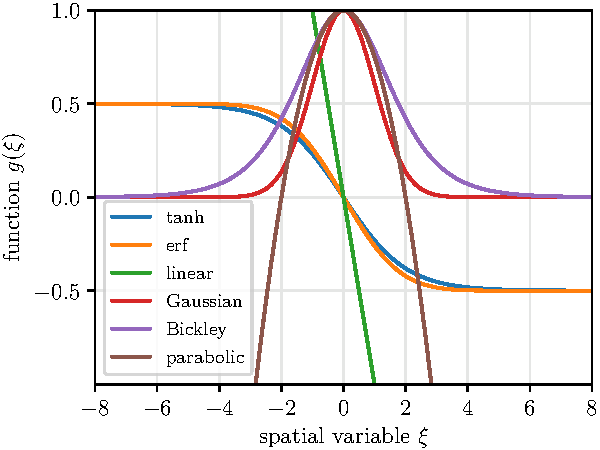
\includegraphics[clip,width=0.6\textwidth]{figs/profiles1}
    \caption{Different normalized profiles used in equation~(\ref{equ:profile}). The black profiles provide shear-like backgrounds, the green lines provide jet-like backgrounds. These background profiles are used consistently for the boundary and initial conditions and aims at the study of different canonical flows, free and wall-bounded, shear- and buoyancy-driven.}\label{fig:profile}
\end{SCfigure}

The second group of profiles deliver a jet-like shape. In that case, $\Delta f$ provides the maximum difference with respect to the reference level $f_\text{ref}$. The integral thickness is defined by
\begin{equation}
    \delta_i =\frac{1}{\Delta f}\int\! (f-f_\text{ref})\,\mathrm{d} x_2
    = \delta\int\! g(\xi)\mathrm{d}\,\xi \;.
    \label{equ:deltai}
\end{equation}
According the implementation currently used, typical values are $\delta_i\sim 2-3\delta$ (table~\ref{tab:profile}).

\begin{table}[!h]
    \footnotesize
    \renewcommand{\arraystretch}{1.2}
    \centering
    \rowcolors{1}{gray!25}{white}
    \begin{tabular}{|l >{\centering}p{0.2\textwidth} c c p{0.4\textwidth}|}
        %
        \hline
        \multicolumn{1}{|>{\columncolor{gray!50}}c}{\bf Type} &
        \multicolumn{1}{>{\columncolor{gray!50}}c}{\bf $\mathbf{g}(\boldsymbol{\xi})$} &
        \multicolumn{1}{>{\columncolor{gray!50}}c}{\bf $\boldsymbol{\delta}_g/\boldsymbol{\delta}$ }&
        \multicolumn{1}{>{\columncolor{gray!50}}c}{\bf $\boldsymbol{\delta}_i/\boldsymbol{\delta}$ }&
        \multicolumn{1}{>{\columncolor{gray!50}}c|}{\bf Notes}\\
        \hline
        Hyperbolic tangent  & $(1/2)\tanh(-\xi/2)$ & $4$ & &
        Used in shear layer because it is the reference profile commonly used in linear stability analysis. The parameter $\delta$ is equal to the momentum thickness. Used because of available linear stability analysis.\\
        Error function      & $(1/2)\text{erf}(-\xi/2)$ & $2\sqrt{\pi}$ & &
        Used in diffusion dominated problems because it is a solution of the diffusion equation.\\
        Linear              & $-\xi$ & 1 & & Varying $\Delta f$ along $\delta$.\\
        Ekman               & $1-\exp(-\xi)\cos(\xi)$ \newline $\phantom{1}-\exp(-\xi)\sin(\xi)$& 1 & &
        Velocity component along geostrophic wind. \newline Normal component.\\
        Gaussian            & $\exp(-\xi^2/2)$ & $1.65$ & $\sqrt{2\pi}$&
        Gaussian bell with standard deviation equal to $\delta$. \\
        Bickley             & $1/\cosh^2(\xi/2)$ & & $4$&
        Bell shape used in the linear stability of jets. Used because of available linear stability analysis.\\
        Parabolic           & $(1+\xi/2)(1-\xi/2)$ & & $8/3$&
        Parabola crossing the reference value at $x_{2,ref}\pm 2\delta$. Used for Poiseuille and channel flows. The thickness $\delta_i$ is calculated using only the positive part of the profile in the integral.\\
        \hline
    \end{tabular}
    \caption{Different normalized profiles used in equation~(\ref{equ:profile}). The third column contains the gradient thickness $\delta_g$, defined by equation~(\ref{equ:deltag}), written explicitly as a function of the thickness parameter $\delta$. The fourth column contains the integral thickness $\delta_i$, defined by equation~(\ref{equ:deltai})}\label{tab:profile}
\end{table}

The are additionally two linear contributions below and above the reference position $x_{2,\text{ref}}$:
\begin{equation}
    f(x_2) = f(x_2)  +\alpha_l (x_2-x_{2,\text{ref}}) \mathcal{H}(x_{2,\text{ref}}-x_2)+\alpha_u (x_2-x_{2,\text{ref}}) \mathcal{H}(x_2-x_{2,\text{ref}})\;,
\end{equation}
where $\mathcal{H}$ is the Heaviside function. The slopes $\alpha_l$ and $\alpha_u$ need to be provided. The default values of the slopes are zero, so that no linear variations are added unless explicitly indicated.

%%%%%%%%%%%%%%%%%%%%%%%%%%%%%%%%%%%%%%%%%%%%%%%%%%%%%%%%%%%%%%%%%%%%%%%%%%%%%%%%
%%%%%%%%%%%%%%%%%%%%%%%%%%%%%%%%%%%%%%%%%%%%%%%%%%%%%%%%%%%%%%%%%%%%%%%%%%%%%%%%
\section{Initial conditions}

White noise is typically added to mean profiles to accelerate the transition to turbulence. There are reasons, however, to construct initial conditions that are more elaborated than white noise:
\begin{itemize}
    \item To be able to compare with analytical solutions and thereby validate the code and algorithms.
    \item To ascertain the duration of the initial transient before the flow enters into the fully developed turbulent regime. We can do that by varying the initial conditions in a controlled way.
    \item To control certain aspects of that transient by using results from stability analysis and exciting or not certain modes. White noise excites all of them equally, and the higher frequency content is dissipated much faster, which might render the energy amount that we use in the initialization misleading. %In this respect, it maybe appropriate to say that the control of the duration of that transient is relatively difficult; on the other hand, the peak of turbulence intensities can be indeed controlled, if necessary e.g. because of resolution constraints.
\end{itemize}

The first step is to defined a mean background profile according to the previous section. For instance, a hyperbolic tangent profile for the mean streamwise velocity, $\bar{u}_1(x_2)$, while all other mean velocity components are set to zero.  The upper stream has a velocity $u_{1,ref}-\Delta u/2$ and the lower stream has a velocity $u_{1,ref}+\Delta u/2$ (see figure~\ref{fig:profile}). The mean density (or the mean temperature) can be similarly initialized, and a mean pressure is set to a uniform value $p_0$. The mean scalar can be similarly initialized.

In addition to the mean values, discrete or broadband perturbation can be added.

\subsection{Discrete Perturbations}

For the general case of a scalar field $s$, we consider the linear superposition of $m$ modes of the form
\begin{equation}
    s_m = A_mf(y) \cos(w_{xm}x+\phi_{xm})\cos(w_{zm}z+\phi_{zm})\;, \\
\end{equation}
where $f(y)$ is one of the shape functions discussed before.

For the particular case of the velocity field, we consider the linear superposition of $m$ modes of the form
\begin{eqnarray}
    u_m &= &A_mg(y)\,c_{xm}         \sin(\omega_{xm}x+\phi_{xm})\cos(\omega_{zm}z+\phi_{zm})\;, \\
    v_m &= &A_mf(y)\phantom{c_{xm}} \cos(\omega_{xm}x+\phi_{xm})\cos(\omega_{zm}z+\phi_{zm})\;, \\
    w_m &= &A_mg(y)\,c_{zm}         \cos(\omega_{xm}x+\phi_{xm})\sin(\omega_{zm}z+\phi_{zm})\;,
\end{eqnarray}
where
\begin{equation*}
    \begin{array}{lll}
        c_{xm}=1/\omega_{xm}    & c_{zm}=0            & \text{if } \omega_{zm}=0\;, \\
        c_{xm}=0           & c_{zm}=1/\omega_{zm}     & \text{if } \omega_{xm}=0\;, \\
        c_{xm}=1/(2\omega_{xm}) & c_{zm}=1/(2\omega_{zm})  & \text{otherwise}\;,
    \end{array}
\end{equation*}
and $g(y)=-f'(y)$. Each mode satisfies the solenoidal constraint.

\subsection{Broadband Perturbations}

We generate a random field on which an isotropic turbulence spectrum  is imposed according to the spectral functions in Table~\ref{tab:spectra}.

\begin{table}[!h]
    \footnotesize
    \renewcommand{\arraystretch}{1.2}
    \centering
    \rowcolors{1}{gray!25}{white}
    \begin{tabular}{|l c p{0.4\textwidth}|}
        %
        \hline
        \rowcolor{gray!50}
        \multicolumn{1}{|>{\columncolor{gray!50}}c}{\bf Type} &
        \multicolumn{1}{>{\columncolor{gray!50}}c}{\bf $E(f)$} &
        \multicolumn{1}{>{\columncolor{gray!50}}c|}{\bf Notes}\\
        uniform   & $1$                                 & ~\\
        quadratic & $(f/f_0)^2 \exp[-2 (f/f_0)]$        & ~\\
        quartic   & $(f/f_0)^4 \exp[-2 (f/f_0)^2]$      & ~\\
        Gaussian  & $\exp[-(1/2)(f/f_0-1)^2/(\sigma/f_0)^2]$ & ~\\
        \hline
    \end{tabular}
    \caption{Different spectral functions that can be used to create a random field. The variable $f$ is the spatial frequency and the parameter $f_0$ is the peak spatial frequency. }\label{tab:spectra}
\end{table}

After these three-dimensional field is created, it is multiplied by a shape function to control the spatial location of this random fluctuation. In case of the velocity field, the solenoidal constraint is imposed on this random field. Such quasi-incompressible fluctuations minimize compressibility transients \cite{Erlebacher:1990}. The pressure fluctuations are obtained from the Poisson equation for incompressible flow.

\begin{SCfigure}
    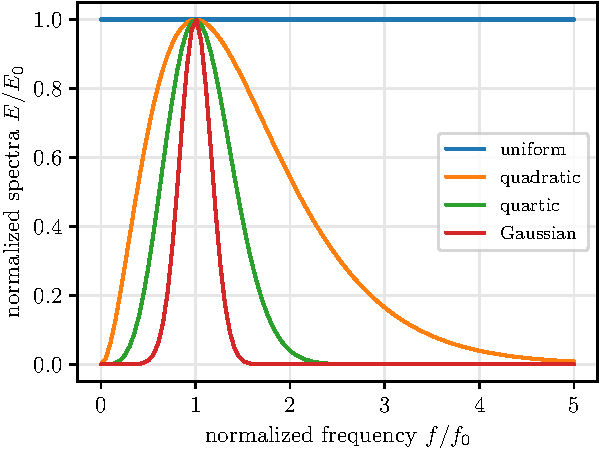
\includegraphics[clip,width=0.6\textwidth]{figs/spectra}
    \caption{Different power spectral densities available as initial conditions, Table~(\ref{tab:spectra}). Normalized such that all of them have equal integral. The Gaussian profile is plotted for the case $\sigma/f_0=1/6$ typically used in the simulations.}
    \label{fig:spectra}
\end{SCfigure}

%%%%%%%%%%%%%%%%%%%%%%%%%%%%%%%%%%%%%%%%%%%%%%%%%%%%%%%%%%%%%%%%%%%%%%%%%%%%%%%%
%%%%%%%%%%%%%%%%%%%%%%%%%%%%%%%%%%%%%%%%%%%%%%%%%%%%%%%%%%%%%%%%%%%%%%%%%%%%%%%%
\section{Boundary conditions}

\subsection{Compressible formulation}

For non-periodic directions, the treatment of the boundary conditions in the
periodic formulation is done in characteristic form
\citep{Thompson:1987,Thompson:1990,Lodato:2008}.

\subsection{Incompressible formulation}

To be developed.

\subsection{Buffer zone}\label{sec:buffer}

Buffer or sponge zones can be considered at the beginning and at the end of the
directions $Ox$ and $Oy$. These are simply defined by specifying the number of
points over which they extend. We can consider a filter or a relaxation form.

Regarding the relaxation form, we simply add
\begin{equation}
    \left(\frac{\delta \mathbf{q}}{\delta t}\right)_b=-\tau_q^{-1}(\mathbf{q}-\mathbf{q}_0)
    \;,\qquad
    \left(\frac{\delta \mathbf{s}}{\delta t}\right)_b=-\tau_s^{-1}(\mathbf{s}-\mathbf{s}_0)
\end{equation}
to the right-hand sides of the transport equations \citep{Hu:1996b}.  The
relaxation times $\tau(\mathbf{x})$ are defined in terms of a power function as
\begin{equation}
    \tau_q^{-1}=\alpha_1(n-n_0)^{\alpha_2} \;,\qquad
    \tau_s^{-1}=\beta_1(n-n_0)^{\beta_2}
\end{equation}
where $n$ is the coordinate normal to the corresponding boundary and $n_0$ the
coordinate where the buffer region begins. The coefficients $\alpha_i$ and
$\beta_i$ need to be provided, the exponents being preferably larger or equal
than 2 so than the pressure equation has a continuous right-hand side.  The
reference fields $\mathbf{q}_0(\mathbf{x})$ and $\mathbf{s}_0(\mathbf{x})$ also
need to be provided and it can be any general field. Normally, a reference field
is created at some moment in the simulation (generally the initial time) as an
average of the corresponding region in the flow and scalar fields.

\chapter{Code}\label{sec:code}

The root directory contains the sources for the common libraries, and the directory {\tt tools} contains the sources for the specific binaries: the main code in {\tt tools/dns}, and the preprocessing and postprocessing tools.

Files {\tt README} and {\tt TODO} contain additional information. To compile, read {\tt INSTALL}.

Directory {\tt examples} contains a few examples to get acquainted with using the code.

%%%%%%%%%%%%%%%%%%%%%%%%%%%%%%%%%%%%%%%%%%%%%%%%%%%%%%%%%%%%%%%%%%%%%%%%%%%%%%%%
%%%%%%%%%%%%%%%%%%%%%%%%%%%%%%%%%%%%%%%%%%%%%%%%%%%%%%%%%%%%%%%%%%%%%%%%%%%%%%%%
\section{Executables}

{
\centering
\setlength{\tabcolsep}{0pt}
\footnotesize

%%%%%%%%%%%%%%%%%%%%%%%%%%%%%%%%%%%%%%%%%%%%%%%%%%%%%%%%%%%%%%%%%%%%%%%%%%%%%%%%
\rowcolors{1}{gray!25}{gray!10}
%
\begin{longtable}{p{0.15\textwidth} p{0.85\textwidth}}
%
\multicolumn{2}{>{\columncolor{lightgreen}}c}{\rule{0pt}{11pt}\normalsize\bf Simulation}\\
%
\tt dns.x &
main program used to run a simulation. It will read its input from the file
dns.ini that the user must supply. An example file is located in {\tt
  examples}. All standard output is written to dns.log and dns.out. Errors are
reported to dns.err and warnings to dns.war. In order to run the simulation you
must provide with an initial flow and scalar fields. and a grid file.\newline
Sources in {\tt tools/dns}.\\
\end{longtable}

%%%%%%%%%%%%%%%%%%%%%%%%%%%%%%%%%%%%%%%%%%%%%%%%%%%%%%%%%%%%%%%%%%%%%%%%%%%%%%%%
\rowcolors{1}{gray!25}{gray!10}
%
\begin{longtable}{p{0.15\textwidth} p{0.85\textwidth}}
%
\multicolumn{2}{>{\columncolor{lightgreen}}c}{\rule{0pt}{11pt}\normalsize\bf Preprocessing}\\
%
\tt inigrid.x &
generates the grid by reading the parameters of the dns.ini
file, section [IniGridOx], [IniGridOy] and [IniGridOz].\newline
Sources in {\tt tools/initialize/grid}.\\
\tt inirand.x &
generates the scal.rand or flow.rand file that contains a
pseudo-random, isotropic field that will be used by the following program to
generate flow or scalar initial fields. The parameters are described in
dns.ini, section [Broadband].\newline Sources in {\tt tools/initialize/rand}\\
\tt iniscal.x &
generates the scal.ics file by reading the parameters of the dns.ini file,
section [IniFields].\newline Sources in {\tt tools/initialize/scal.}\\
\tt iniflow.x &
generates the flow.ics file by reading the parameters of the dns.ini file,
section [IniFields].\newline Sources in {\tt tools/initialize/flow}.\\
\end{longtable}

%%%%%%%%%%%%%%%%%%%%%%%%%%%%%%%%%%%%%%%%%%%%%%%%%%%%%%%%%%%%%%%%%%%%%%%%%%%%%%%%
\rowcolors{1}{gray!25}{gray!10}
%
\begin{longtable}{p{0.15\textwidth} p{0.85\textwidth}}
%
\multicolumn{2}{>{\columncolor{lightgreen}}c}{\rule{0pt}{11pt}\normalsize\bf Postprocessing}\\
%
\tt averages.x &
calculates main average profiles and conditional averages (outer intermittency).\newline
Sources in {\tt tools/statistics/averages}.\\
\tt spectra.x &
calculates 1D, 2D and 3D spectra and co-spectra of main variables. Correlations should be
included here.\newline
Sources in {\tt tools/statistics/spectra}.\\
\tt pdfs.x &
calculates PDFs, joints PDFs and conditional PDFs.\newline
Sources in {\tt tools/statistics/pdfs}.\\
\tt visuals.x &
calculates different fields and exports data for visualization (default is
ensight format). \newline
Sources in {\tt tools/plot/visuals}.\\
\end{longtable}

}

\pagebreak

%%%%%%%%%%%%%%%%%%%%%%%%%%%%%%%%%%%%%%%%%%%%%%%%%%%%%%%%%%%%%%%%%%%%%%%%%%%%%%%%
%%%%%%%%%%%%%%%%%%%%%%%%%%%%%%%%%%%%%%%%%%%%%%%%%%%%%%%%%%%%%%%%%%%%%%%%%%%%%%%%
\section{Scripts}

Sources in {\tt scripts/python}.

{
\centering
\setlength{\tabcolsep}{0pt}
\footnotesize

%%%%%%%%%%%%%%%%%%%%%%%%%%%%%%%%%%%%%%%%%%%%%%%%%%%%%%%%%%%%%%%%%%%%%%%%%%%%%%%%
\rowcolors{1}{gray!25}{gray!10}
%
\begin{longtable}{p{0.15\textwidth} p{0.85\textwidth}}
%
\multicolumn{2}{>{\columncolor{lightred}}c}{\rule{0pt}{11pt}\normalsize\bf Python}\\
%
\tt xdmf.py &
Create XDMF file with fields data for visualization tools, such as ParaView. Argument is the list of binary files to be included in the XDMF file. Edit the file to set grid size.\\
\tt xdmfplanes.py &
Create XDMF file with planes data for visualization tools, such as ParaView. Argument is the list of binary files to be included in the XDMF file. Edit the file to set grid size and plane parameters.\\
\tt stats2nc.py &
Construct NetCDF files from a list of ASCII statistics files.\\
\end{longtable}

}

%%%%%%%%%%%%%%%%%%%%%%%%%%%%%%%%%%%%%%%%%%%%%%%%%%%%%%%%%%%%%%%%%%%%%%%%%%%%%%%%
%%%%%%%%%%%%%%%%%%%%%%%%%%%%%%%%%%%%%%%%%%%%%%%%%%%%%%%%%%%%%%%%%%%%%%%%%%%%%%%%
\section{Input file dns.ini}

The following tables describe the different blocks appearing in the input file {\tt dns.ini}. The first column contains the tag. The second column contains the possible values, the first one being the default one and the word {\it value} indicating that a numerical value needs to be provided. The third column describes the field. This data is read in the file {\tt *\_READ\_GLOBAL} and in the files {\tt *\_READ\_LOCAL} of each of the tools; the variable corresponding to each field should be also read there.

Data is case insensitive.

{
\centering
\setlength{\tabcolsep}{0pt}
\footnotesize

%%%%%%%%%%%%%%%%%%%%%%%%%%%%%%%%%%%%%%%%%%%%%%%%%%%%%%%%%%%%%%%%%%%%%%%%%%%%%%%%
\rowcolors{1}{gray!25}{gray!10}
%
\begin{longtable}{p{0.15\textwidth} p{0.3\textwidth} p{0.55\textwidth}}
%
\multicolumn{3}{>{\columncolor{lightblue}}c}{\normalsize\bf [Version]}\\
%
\tt Major & {\it value} &
Major version number. An error is generated if different from the value set in
{\tt DNS\_READ\_GLOBAL}.\\
\tt Minor & {\it value} &
Minor version number. A warning is generated if different from the value set in
{\tt DNS\_READ\_GLOBAL}.\\
\end{longtable}

%%%%%%%%%%%%%%%%%%%%%%%%%%%%%%%%%%%%%%%%%%%%%%%%%%%%%%%%%%%%%%%%%%%%%%%%%%%%%%%%
\rowcolors{1}{gray!25}{gray!10}
%
\begin{longtable}{p{0.15\textwidth} p{0.3\textwidth} p{0.55\textwidth}}
%
\multicolumn{3}{>{\columncolor{lightblue}}c}{\normalsize\bf [Main]}\\
%
\tt Type & \tt temporal, spatial      &
Temporally evolving or spatially evolving simulation.\\
\tt Flow & \tt shear, jet, isotropic &
Flow geometry, mainly related to initial and boundary conditions.\\
\tt CalculateFlow & \tt yes, no &
Execute code segments affecting flow variables.\\
\tt CalculateScalar & \tt yes, no &
Execute code segments affecting scalar variables.\\
\tt Equations & \tt internal, total, incompressible &
Define system of equations to be solved.\\
\tt Mixture & \tt None, AirVapor, AirWater, AirWaterLinear &
Defines the mixture to be used for the thermodynamics.\\
\tt TermAdvection & \tt divergence, convective, skewsymmetric &
Formulation of advection terms.\\
\tt TermViscous & \tt divergence, explicit&
Formulation of viscous terms.\\
\tt TermDiffusion & \tt divergence, explicit &
Formulation of diffusion terms.\\
\tt TermBodyForce & \tt None, Explicit, Homogeneous, Linear, Bilinear,
Quadratic &
Formulation of body force terms (see {\tt mappings/fi\_buoyancy}).\\
\tt TermCoriolis & \tt None, Explicit, Normalized &
Formulation of Coriolis terms.\\
\tt TermRadiation & \tt None, Bulk1dGlobal, Bulk1dLocal &
Formulation of radiation terms (see {\tt operators/opr\_radiation}).\\
\tt SpaceOrder & \tt CompactJacobian4, CompactJacobian6, CompactDirect6 &
Finite difference method used for spatial derivatives.\\
\tt TimeOrder & \tt RungeKuttaExplicit3, RungeKuttaExplicit4, RungeKuttaDiffusion3 &
Runge-Kutta method used for time advancement.\\
\tt TimeStep & {\it value} &
If positive, constant time step to be used in time marching scheme.\\
\tt TimeCFL & {\it value} & Courant number for the advection part.\\
\end{longtable}

%%%%%%%%%%%%%%%%%%%%%%%%%%%%%%%%%%%%%%%%%%%%%%%%%%%%%%%%%%%%%%%%%%%%%%%%%%%%%%%%
\rowcolors{1}{gray!25}{gray!10}
%
\begin{longtable}{p{0.15\textwidth} p{0.3\textwidth} p{0.55\textwidth}}
%
\multicolumn{3}{>{\columncolor{lightblue}}c}{\normalsize\bf [Iteration]}\\
%
\tt Start & {\em value} & Initial iteration. The corresponding files {\tt flow.*}
and {\tt scal.*} will be read from disk.\\
\tt End & {\em value} & Final iteration at which the algorithm will be stopped.\\
\tt Restart & {\em value} & Iteration-step frequency to write the restart files to disk.\\
\tt Statistics & {\em value} & Iteration-step frequency to calculate statistics.\\
\tt IteraLog& {\em value} & Iteration-step frequency to write the log-file {\tt dns.out}.\\
\tt SavePlanes& {\em value} & Iteration-step frequency to write plane data to disk.\\
\tt RunAvera& \tt no, yes & Save running averages to disk (spatially evolving simulations).\\
\tt RunLines& \tt no, yes & Save line information to disk (spatially evolving simulations).\\
\tt RunPlane& \tt no, yes & Save plane information to disk (spatially evolving simulations).\\
\tt StatSave& {\em value} &  Iteration-step frequency to accumulate statistics (spatially evolving simulations).\\
\tt StatStep& {\em value} & Iteration-step frequency to save statistics to disk (spatially evolving simulations).\\
\end{longtable}

%%%%%%%%%%%%%%%%%%%%%%%%%%%%%%%%%%%%%%%%%%%%%%%%%%%%%%%%%%%%%%%%%%%%%%%%%%%%%%%%
\rowcolors{1}{gray!25}{gray!10}
%
\begin{longtable}{p{0.15\textwidth} p{0.3\textwidth} p{0.55\textwidth}}
%
\multicolumn{3}{>{\columncolor{lightblue}}c}{\normalsize\bf [Parameters]}\\
%
\tt Reynolds & {\em value} & Reynolds number $\mathbf{Re}$ (see section~\ref{sec:equations}).\\
\tt Prandtl  & {\em value} & Prandtl number $\mathbf{Pr}$.\\
\tt Froude   & {\em value} & Froude number $\mathbf{Fr}$.\\
\tt Rossby   & {\em value} & Rossby number $\mathbf{Ro}$.\\
\tt Mach     & {\em value} & Mach number $\mathbf{Ma}$.\\
\tt Gama     & {\em value} & Ratio of specific heats $\gamma$.\\
\tt Schmidt  & {\em value1, value2, ...} & List of Schmidt numbers $\mathbf{Sc}_i$. The number of values defines the number of scalars. If a mixture is defined in the block [Main], then consistency is checked.\\
\tt Damkohler & {\em value1, value2, ...} & List of Damkohler numbers $\mathbf{Da}_i$.\\
\end{longtable}

%%%%%%%%%%%%%%%%%%%%%%%%%%%%%%%%%%%%%%%%%%%%%%%%%%%%%%%%%%%%%%%%%%%%%%%%%%%%%%%%
\rowcolors{1}{gray!25}{gray!10}
%
\begin{longtable}{p{0.15\textwidth} p{0.3\textwidth} p{0.55\textwidth}}
%
\multicolumn{3}{>{\columncolor{lightblue}}c}{\normalsize\bf [Control]}\\
%
\tt FlowLimit & \tt yes, no & Monitor and eventually force the thermodynamic
fields to be  within a prescribed interval.\\
\tt MinPressure & {\em value} & Lower bound for the pressure interval.\\
\tt MaxPressure & {\em value} & Upper bound for the pressure interval.\\
\tt MinDensity & {\em value} & Lower bound for the density interval.\\
\tt MaxDensity & {\em value} & Upper bound for the density interval.\\
ScalLimit  & \tt yes, no & Monitor and eventually force the scalar fields to be
within a prescribed interval.\\
\tt MinScalar & {\em value} & Lower bound for the scalar interval.\\
\tt MaxScalar & {\em value} & Upper bound for the scalar interval.\\
\end{longtable}

%%%%%%%%%%%%%%%%%%%%%%%%%%%%%%%%%%%%%%%%%%%%%%%%%%%%%%%%%%%%%%%%%%%%%%%%%%%%%%%%
\rowcolors{1}{gray!25}{gray!10}
%
\begin{longtable}{p{0.15\textwidth} p{0.3\textwidth} p{0.55\textwidth}}
%
\multicolumn{3}{>{\columncolor{lightblue}}c}{\normalsize\bf [Grid]}\\
%
\tt Imax & {\it value} & Number of points along the Ox direction (first array
index).\\
\tt Jmax & {\it value} & Number of points along the Oy direction (second array
index).\\
\tt Kmax & {\it value} & Number of points along the Oz direction (third array
index).\newline If set equal to 1, then 2D simulation.\\
\tt Imax(*) & {\it value} & Number of points per processor (MPI task) along the Ox
direction (MPI parallel mode).\\
\tt Jmax(*) & {\it value} & Number of points per processor (MPI task) along the Oy
direction (MPI parallel mode). So far, this value is set equal to the total size
because only a 2D decomposition has been implemented.\\
\tt Kmax(*) & {\it value} & Number of points per processor (MPI task) along the
Oz direction (MPI parallel mode).\\
\tt XUniform & \tt yes, no & If yes, no Jacobian information is needed in Ox direction.\\
\tt YUniform & \tt yes, no & If yes, no Jacobian information is needed in Oy direction.\\
\tt ZUniform & \tt yes, no & If yes, no Jacobian information is needed in Oz direction.\\
\tt XPeriodic & \tt yes, no & Periodicity along Ox direction.\\
\tt YPeriodic & \tt yes, no & Periodicity along Oy direction.\\
\tt ZPeriodic & \tt yes, no & Periodicity along Oz direction.\\
\end{longtable}

%%%%%%%%%%%%%%%%%%%%%%%%%%%%%%%%%%%%%%%%%%%%%%%%%%%%%%%%%%%%%%%%%%%%%%%%%%%%%%%%
\rowcolors{1}{gray!25}{gray!10}
%
\begin{longtable}{p{0.15\textwidth} p{0.3\textwidth} p{0.55\textwidth}}
%
\multicolumn{3}{>{\columncolor{lightblue}}c}{\normalsize\bf [BoundaryConditions]}\\
%
\tt VelocityImin & \tt none, noslip, freeslip & Velocity boundary condition at $x_\text{min}$
(incompressible mode).\\
\tt VelocityImax & \tt none, noslip, freeslip & Velocity boundary condition at $x_\text{max}$
(incompressible mode).\\
\tt Scalar\#Imin & \tt none, dirichlet, neumman & Scalar boundary condition at $x_\text{min}$
(incompressible mode). The symbol {\tt \#} is the number of the scalar.\\
\tt Scalar\#Imax & \tt none, dirichlet, neumman & Scalar boundary condition at $x_\text{max}$
(incompressible mode). The symbol {\tt \#} is the number of the scalar.\\
\multicolumn{3}{l}{\it Similarly in the other directions $Oy$ and $Oz$.}\\
\multicolumn{3}{l}{Compressible-case information to be filled.}\\
\end{longtable}

%%%%%%%%%%%%%%%%%%%%%%%%%%%%%%%%%%%%%%%%%%%%%%%%%%%%%%%%%%%%%%%%%%%%%%%%%%%%%%%%
\rowcolors{1}{gray!25}{gray!10}
%
\begin{longtable}{p{0.15\textwidth} p{0.3\textwidth} p{0.55\textwidth}}
%
\multicolumn{3}{>{\columncolor{lightblue}}c}{\normalsize\bf [BufferZone]}\\
%
\tt Type & \tt none, relaxation, filter, both & Type of buffer or sponge layer
to use.\\
\tt LoadBuffer & \tt no, yes & If {\tt no}, then create reference buffer fields
from the current fields and save them to disk.\newline
If {\tt yes}, then read the necessary buffer fields from disk. E.g., for the
upper boundary, the file name to be searched for would be {\tt flow.bcs.jmax}
and {\tt scal.bcs.jmax}.\\
\tt PointsImin & {\em value} & Number of points in the $Ox$ direction at $x_\text{min}$.\\
\tt PointsImax & {\em value} & Number of points in the $Ox$ direction at $x_\text{max}$.\\
\tt PointsUJmin & {\em value} & Number of points in the $Oy$ direction at
$y_\text{min}$ for the velocity fields.\\
\tt PointsUJmax & {\em value} & Number of points in the $Oy$ direction at
$y_\text{max}$ for the velocity fields.\\
\tt PointsEJmin & {\em value} & Number of points in the $Oy$ direction at
$y_\text{min}$ for the thermodynamic fields.\\
\tt PointsEJmax & {\em value} & Number of points in the $Oy$ direction at
$y_\text{max}$ for the thermodynamic fields.\\
\tt PointsSJmin & {\em value} & Number of points in the $Oy$ direction at
$y_\text{min}$ for the scalar fields.\\
\tt PointsSJmax & {\em value} & Number of points in the $Oy$ direction at
$y_\text{max}$ for the scalar fields.\\
\tt ParametersU & {\em value1, value2, ...} & Set of parameters defining strength and exponent of the relaxation term in the flow and
thermodynamic fields, section~\ref{sec:buffer}.\\
\tt ParametersS & {\em value1, value2, ...} & Set of parameters defining strength and exponent of the relaxation term in the scalar fields,
section~\ref{sec:buffer}.\\
\end{longtable}

%%%%%%%%%%%%%%%%%%%%%%%%%%%%%%%%%%%%%%%%%%%%%%%%%%%%%%%%%%%%%%%%%%%%%%%%%%%%%%%%
\rowcolors{1}{gray!25}{gray!10}
%
\begin{longtable}{p{0.15\textwidth} p{0.3\textwidth} p{0.55\textwidth}}
%
\multicolumn{3}{>{\columncolor{lightblue}}c}{\normalsize\bf [Flow]}\\
%
\tt Pressure  & {\em value} & Reference mean pressure.\\
\tt Density   & {\em value} & Reference mean density.\\
\tt VelocityX & {\em value} & Reference mean velocity along $Ox$.\\
\tt VelocityY & {\em value} & Reference mean velocity along $Oy$.\\
\tt VelocityZ & {\em value} & Reference mean velocity along $Oz$.\\
%
\tt ProfileVelocity & \tt None, Linear, Tanh, Erf, Ekman, EkmanP &
Function form of the mean velocity profile, typically along the direction
$Ox$.\\
\tt YCoorVelocity & {\em value} & Coordinate along $Oy$ of the reference point
of the profile, relative to the total scale, equation~(\ref{equ:profile}).\\
\tt ThickVelocity & {\em value} & Reference profile thickness, equation~(\ref{equ:profile}).\\
\tt DeltaVelocity & {\em value} & Reference profile difference,
equation~(\ref{equ:profile}).\\
\tt DiamVelocity  & {\em value} & Reference profile diameter (jet mode).\\
%
\multicolumn{3}{l}{\it Similarly for density or temperature}\\
%
\end{longtable}

%%%%%%%%%%%%%%%%%%%%%%%%%%%%%%%%%%%%%%%%%%%%%%%%%%%%%%%%%%%%%%%%%%%%%%%%%%%%%%%%
\rowcolors{1}{gray!25}{gray!10}
%
\begin{longtable}{p{0.15\textwidth} p{0.3\textwidth} p{0.55\textwidth}}
%
%
\multicolumn{3}{>{\columncolor{lightblue}}c}{\normalsize\bf [Scalar]}\\
%
\tt ProfileScalar\# & \tt None, Linear, Tanh, Erf, LinearErf &
Function form of the mean profile.\\
\tt MeanScalar\# & {\em value} & Reference mean scalar.\\
\tt YCoorScalar\# & {\em value} & Coordinate along $Oy$ of the reference point
of the profile, relative to the total scale.\\
\tt ThickScalar\# & {\em value} & Reference profile thickness.\\
\tt DeltaScalar\# & {\em value} & Reference profile difference.\\
\tt DiamScalar\#  & {\em value} & Reference profile diameter (jet mode).\\
%
\end{longtable}

%%%%%%%%%%%%%%%%%%%%%%%%%%%%%%%%%%%%%%%%%%%%%%%%%%%%%%%%%%%%%%%%%%%%%%%%%%%%%%%%
\rowcolors{1}{gray!25}{gray!10}
%
\begin{longtable}{p{0.15\textwidth} p{0.3\textwidth} p{0.55\textwidth}}
%
\multicolumn{3}{>{\columncolor{lightblue}}c}{\normalsize\bf [BodyForce]}\\
%
\tt Vector     & {\em value1, value2, value3} & Components of the buoyancy
unitary vector $(g_1,\,g_2,\,g_3)$ in section~\ref{sec:equations}.\\
\tt Parameters & {\em value1, value2, ...} & Set of parameters defining the
buoyancy function $b^e(s_i)$.\\
\end{longtable}

%%%%%%%%%%%%%%%%%%%%%%%%%%%%%%%%%%%%%%%%%%%%%%%%%%%%%%%%%%%%%%%%%%%%%%%%%%%%%%%%
\rowcolors{1}{gray!25}{gray!10}
%
\begin{longtable}{p{0.15\textwidth} p{0.3\textwidth} p{0.55\textwidth}}
%
\multicolumn{3}{>{\columncolor{lightblue}}c}{\normalsize\bf [Rotation]}\\
%
\tt Vector     & {\em value1, value2, value3} & Components of the angular
velocity vector $(f_1,\,f_2,\,f_3)$ in section~\ref{sec:equations}.\\
\tt Parameters & {\em value1, value2, ...} & Set of parameters defining the Coriolis
force term.\\
\end{longtable}

%%%%%%%%%%%%%%%%%%%%%%%%%%%%%%%%%%%%%%%%%%%%%%%%%%%%%%%%%%%%%%%%%%%%%%%%%%%%%%%%
\rowcolors{1}{gray!25}{gray!10}
%
\begin{longtable}{p{0.15\textwidth} p{0.3\textwidth} p{0.55\textwidth}}
%
\multicolumn{3}{>{\columncolor{lightblue}}c}{\normalsize\bf [Radiation]}\\
%
\tt Scalar & {\em value} & Index of scalar field on which the effect of
radiation heating or cooling is acting.\\
\tt Parameters & {\em value1, value2, ...} & Set of parameters defining the
radiation function $r^e(s_i)$.\\
\end{longtable}

%%%%%%%%%%%%%%%%%%%%%%%%%%%%%%%%%%%%%%%%%%%%%%%%%%%%%%%%%%%%%%%%%%%%%%%%%%%%%%%%
\rowcolors{1}{gray!25}{gray!10}
%
\begin{longtable}{p{0.15\textwidth} p{0.3\textwidth} p{0.55\textwidth}}
%
\multicolumn{3}{>{\columncolor{lightblue}}c}{\normalsize\bf [IniFields]}\\
%
\tt Velocity & \tt None, VelocityDiscrete, VelocityBroadband,
VorticityBroadband, PotentialBroadband & Type of initial velocity field.\\
\tt Temperature & \tt None, PlaneBroadband, PlaneDiscrete &
Type of initial temperature field.\\
\tt Scalar & \tt None, LayerDiscrete, LayerBroadband, PlaneDiscrete,
PlaneBroadband, DeltaDiscrete, DeltaBroadband, FluxDiscrete, FluxBroadband &
Type of initial scalar field.\\
\tt ForceDilatation & \tt yes, no & Force the velocity field to satisfy the
solenoidal constraint.\\
\tt ProfileIni\{K,S\} & \tt Gaussian, Parabolic, ... & Type of modulation along Oy of perturbation field.\\
\tt ThickIni & {\em value}[{\em1 , value2, ...}]& Thickness of fluctuation shape
profile. The mean profile is set by the corresponding values in {\tt [Flow]} and
{\tt [Scalar]}. In case of the scalar, as many values as scalars should be
provided. You can differentiate between flow and scalar values by using {\tt ThickIniK} and {\tt ThickIniS}.\\
\tt YCoorIni & {\em value}[{\em1 , value2, ...}] & Coordinate along $Oy$ of the
reference point of the fluctuation shape profile, relative to the total
scale. The mean profile is set by the corresponding values in {\tt [Flow]} and
{\tt [Scalar]}. In case of the scalar, as many values as scalars should be
provided. You can differentiate between flow and scalar values by using {\tt YCoorIniK} and {\tt YCoorIniS}. The default values are those specified in {\tt [Flow]} and
{\tt [Scalar]}.\\
\tt NormalizeK & {\em value} & Maximum value of the profile of the turbulent
kinetic energy.\\
\tt NormalizeP & {\em value} & Maximum value of the profile of the pressure
root-mean-square.\\
\tt NormalizeS & {\em value1, value2, ...} & Maximum value of the profile of the
scalar
root-mean-square.\\
\tt Mixture & \tt None, Equilibrium, LoadFields & Type of mixture with which to
initialize the thermodynamic fields.\\
\end{longtable}

% %%%%%%%%%%%%%%%%%%%%%%%%%%%%%%%%%%%%%%%%%%%%%%%%%%%%%%%%%%%%%%%%%%%%%%%%%%%%%%%%
\rowcolors{1}{gray!25}{gray!10}
%
\begin{longtable}{p{0.15\textwidth} p{0.3\textwidth} p{0.55\textwidth}}
  %
  \multicolumn{3}{>{\columncolor{lightblue}}c}{\normalsize\bf [Filter]}\\
  %
  \tt Type & \tt None, Adm, Helmholtz, TopHat, Compact, Explicit6, Explicit4, SpectralBand, SpectralErf & Type of filter used in simulation (if any) and postprocessing.\\
  \tt Parameters & {\em value1, value2, ...} & Values defining the filter, e.g., $\alpha$ in compact, or $\Delta$ in tophat.\\
  \tt ActiveY & \tt yes,no & Active or not in direction $Oy$.\\
  \tt BcsJmin & \tt Free, Solid & Type of boundary condition for tophat filter at $y_\text{min}$. Other filters might have other options, as explained in section~\ref{sec:filters}.\\
  \tt BcsJmax & \tt Free, Solid & Type of boundary condition for tophat filter at $y_\text{max}$. Other filters might have other options, as explained in section~\ref{sec:filters}.\\
\multicolumn{3}{l}{\it Similarly in the other directions $Ox$ and $Oz$.}\\
\end{longtable}

%%%%%%%%%%%%%%%%%%%%%%%%%%%%%%%%%%%%%%%%%%%%%%%%%%%%%%%%%%%%%%%%%%%%%%%%%%%%%%%%
\rowcolors{1}{gray!25}{gray!10}
%
\begin{longtable}{p{0.15\textwidth} p{0.3\textwidth} p{0.55\textwidth}}
%
\multicolumn{3}{>{\columncolor{lightblue}}c}{\normalsize\bf [Broadband]}\\
%
\tt Type & \tt None, Physical, Phase & Randomness is set in physical
space, or in the phase in frequency space. \\
\tt Distribution & uniform, gaussian & Type of probability density function (PDF).\\
\tt Seed & {\it value} & Seed for the random generator.\\
\tt Covariance & {\it value1, value2, ...} & Flow covariance matrix.\\
\tt Spectrum & \tt uniform, quadratic, quartic, gaussian & Form of the power
spectral density, equation~(\ref{equ:spectra}).\\
\tt f0 & {\it value} & Parameters defining the functional form of the power
spectral density.\\
\end{longtable}

%%%%%%%%%%%%%%%%%%%%%%%%%%%%%%%%%%%%%%%%%%%%%%%%%%%%%%%%%%%%%%%%%%%%%%%%%%%%%%%%
\rowcolors{1}{gray!25}{gray!10}
%
\begin{longtable}{p{0.15\textwidth} p{0.3\textwidth} p{0.55\textwidth}}
%
\multicolumn{3}{>{\columncolor{lightblue}}c}{\normalsize\bf [Discrete]}\\
%
\tt Amplitude   & {\it value1, value2, ...} & Amplitude of the modes.\\
\tt ModeX       & {\it value1, value2, ...} & Mode numbers as multiples of fundamental frequency along Ox.\\
\tt ModeZ       & {\it value1, value2, ...} & Mode numbers as multiples of fundamental frequency along Oz.\\
\tt PhaseX      & {\it value1, value2, ...} & Corresponding phases.\\
\tt PhaseZ      & {\it value1, value2, ...} & Corresponding phases.\\
\tt Type        &  \tt Varicose, Sinuous, Gaussian & Modulation of the sinusoidal perturbation.\\
\tt Parameters  & {\it value} & Parameters that define the modulation.\\
\end{longtable}

%% \item \textbf{3DAmpl} (\textit{A3d}): intensity.
%% \item \textbf{3DXPhi} (\textit{Phix3d}): Same as above, but for the 3D pertubations.
%% \item \textbf{3DZPhi} (\textit{Phiz3d}): Same as above.


% %%%%%%%%%%%%%%%%%%%%%%%%%%%%%%%%%%%%%%%%%%%%%%%%%%%%%%%%%%%%%%%%%%%%%%%%%%%%%%%%
\rowcolors{1}{gray!25}{gray!10}
%
\begin{longtable}{p{0.15\textwidth} p{0.3\textwidth} p{0.55\textwidth}}
  %
  \multicolumn{3}{>{\columncolor{lightblue}}c}{\normalsize\bf [Inflow]}\\
  %
  \tt Type & \tt None, Discrete, BroadbandPeriodic,  BroadbandSequential & Type of
  inflow forcing to use
  in a spatially evolving simulation.\\
  \tt Adapt & \it value & Interval in global time units for starting the inflow
  forcing.\\
\end{longtable}

%%%%%%%%%%%%%%%%%%%%%%%%%%%%%%%%%%%%%%%%%%%%%%%%%%%%%%%%%%%%%%%%%%%%%%%%%%%%%%%%
\rowcolors{1}{gray!25}{gray!10}
%
\begin{longtable}{p{0.15\textwidth} p{0.3\textwidth} p{0.55\textwidth}}
%
\multicolumn{3}{>{\columncolor{lightblue}}c}{\normalsize\bf [PostProcessing]}\\
%
\tt Files     & {\it value1, value2, ...} & Iterations to be postprocessed.\\
\tt Subdomain & $i_{1}, i_{2}, j_{1}, j_{2}, k_{1}, k_{2}$ &
Grid block to be postprocessed.\\
\tt Partition & $\alpha_1$[, $\alpha_2$], $\beta_1$, ..., $\beta_{n-1}$&
Type of partition defined by values \{$\alpha_1$[, $\alpha_2$]\}. The first
parameter defines the conditioning field: 1. external field, 2. scalar field,
3. enstrophy, 4. magnitude of scalar gradient. The second parameter chooses
between a relative or an absolute threshold values. Set of thresholds
\{$\beta_1$, ...,$\beta_{n-1}$\} to define the partition of the conditioning
field into $n$ zones.\\
\tt ParamAverages & $\alpha_1$[, $\alpha_2$, $\alpha_3$, $\alpha_4$]& Main option
$\alpha_1$ (see {\tt tools/statistics/averages.f90}); block size $\alpha_2$; gate
level $\alpha_3$; maximum order of the moments $\alpha_4$.\\
\tt ParamPdfs & $\alpha_1$[, $\alpha_2$, $\alpha_3$, $\alpha_4$]& Main option
$\alpha_1$ (see {\tt tools/statistics/pdfs.f90}); block size $\alpha_2$; gate
level $\alpha_3$; number of bins $\alpha_4$.\\
\tt ParamSpectra & $\alpha_1$[, $\alpha_2$, $\alpha_3$, $\alpha_4$]& Main option
$\alpha_1$ (see {\tt tools/statistics/spectra.f90}); block size
$\alpha_2$; save full spectra $\alpha_3$; average over iterations $\alpha_4$.\\
\tt ParamVisuals & $\alpha_1,\,\alpha_2,\,\ldots$ & List of fields to be calculated (see {\tt tools/plot/visuals.f90}).\\
\end{longtable}

}

% {\Large\bf [Statistics]}

% \begin{itemize}
% \item \textbf{FilterEnergy} (\textit{ffltdmp}):  If ``yes'' calculate corresponding statistics.(default=no)
% \item \textbf{EpsInter} (\textit{eps\_inter}): (default=0.01)
% \item \textbf{IAvera} (\textit{statavg}): Planes i constant to be averaged.(default=1)
% \item \textbf{ILines} (\textit{statlin\_i}): I position of line to be saved. It has to match with JLines.(default=1)
% \item \textbf{JLines} (\textit{statlin\_j}): J position of line to be saved. It has to match with ILines. (default=1)
% \item \textbf{IPlane} (\textit{statpln}): Planes i constant to be saved. (default=1)
% \end{itemize}

% %%%%%%%%%%%%%%%%%%%%%%%%%%%%%%%%%%%%%%%%%%%%%%%%%%%%%%%%%%%%%%%%%%%%%%%%%%%%%%%%
% {\Large\bf [LES]}

% \begin{itemize}
% \item \textbf{Active} (\textit{iles}): ``yes'' if SGS terms are used. (default=no)
% \item \textbf{Transport}  (\textit{iles\_type\_tran}): ``none'', ``ssm'' for scale similarity , ``arm-rans'' for approximate reconstruction, ``arm-sptl'' for approximate reconstruction, ``arm-invs'' (default=ssm)
% \item \textbf{Regularization} (\textit{iles\_type\_regu}): ``none'', ``smg-static'', ``smg-dynamic'', ``smg-static-rms'', ``smg-dynamic-rms'' (default=smg-static)
% \item \textbf{Dissipation} (\textit{iles\_type\_diss}): ``none'', ``diss-sgs'' (default=none)
% \item \textbf{Chemistry} (\textit{iles\_type\_chem}):  ``none'', ``arm\_bs arm\_ps'' (default=none)
% \item \textbf{Filter0Size} (\textit{isgs\_f0size}): $\Delta\_f / \Delta\_g$ of filter level 0. Integer even number. (default=2)
% \item \textbf{Filter1Size} (\textit{isgs\_f1size}): $\Delta\_f / \Delta\_g$ of filter level 1. Integer even number. (default=4)
% \item \textbf{Inviscid} (\textit{iles\_inviscid}): (default=no)
% \item \textbf{JmaxDeact} (\textit{iles\_jmaxdeact}): (default=1)
% \item \textbf{SmagVariant} (\textit{sgs\_devsmag}): ``deviatoric'' for Smagorinsky expression in terms of the deviatoric tensors (``other'' for relation in the whole tensor). (default=deviatoric)
% \item \textbf{SmagTrans} (\textit{sgs\_smagtrans}): (default=-1.0)
% \item \textbf{SmagDelta} (\textit{sgs\_smagdelta}): (default=0.0)
% \item \textbf{Alpha} (\textit{sgs\_alpha}): Constant for scale similarity model.(default=1.0)
% \item \textbf{Csm} (\textit{sgs\_csm}): Smagorinsky constant.(default=0.13)
% \item \textbf{Prs} (\textit{sgs\_prs}): Smagorinsky Prandtl number. (default=0.6)
% \item \textbf{Sct} (\textit{sgs\_sct}): Smagorinsky Schmidt number. (default=0.6)
% \item \textbf{AlphaDil} (\textit{sgs\_pdil}): (default=2.2)
% \item \textbf{ChemistryCondDissipation} (\textit{iles\_type\_disZchem}): Conditonal dissipation model. ``mean'', ``one-dimensional'' (default=mean)
% \item \textbf{ChemistryDissipation} (\textit{iles\_type\_dischem}): Dissipation model. ``gradient'', ``diss-sgs'' (default=gradient)
% \item \textbf{FDFfile} (\textit{les\_fdf\_bs\_file}): file name
% \item \textbf{ChemistryVariance} (\textit{iles\_type\_recchem}): ssm arm-invs arm-rans arm-sptl (default=arm-rans)
% \item \textbf{ARM\_Spectrum} (\textit{iarm\_spc}): Type of model spectrum; ``Pope'' or ``adhoc''. (default=Pope)
% \item \textbf{ARM\_NL} (\textit{iarm\_nl}): Number of points in gamma for the c0-table.(default=10)
% \item \textbf{ARM\_NRe} (\textit{iarm\_nre}): Number of points in Reynolds for the c0-table. (default=10)
% \item \textbf{ARM\_ReMin} (\textit{arm\_remin}): Minimun Reynolds for the c0-table (default=10.0)
% \item \textbf{ARM\_DeltaRe} (\textit{arm\_dre}): Increment in the Reynolds for the c0-table.(default=10.0)
% \item \textbf{ARM\_ActivaT} (\textit{arm\_tact}): (default=100)
% \item \textbf{ARM\_FlameT} (\textit{arm\_tflame}): (default=10)
% \item \textbf{ARM\_StechioZ} (\textit{arm\_zst}): (default=0.2)
% \item \textbf{ARM\_SmoothZ} (\textit{arm\_smooth}): (default=0.1)
% \item \textbf{ARM\_c0} (\textit{arm\_c0\_inviscid}): (default=4.72)
% \end{itemize}

\chapter{Grid}\label{sec:grid}

The equations are solved using Cartesian co-ordinates and the grid is structured. The grid is constructed by building up the three directions separately (in a 2D case, $Oz$ has simply one node).  Each direction is broken into segments, and each of those segments is built with specified generation algorithms. The first node in each direction is set at zero. 

The executable is {\tt inigrid.x} and the data in {\tt dns.ini} is specified in the blocks [IniGridOx], [IniGridOy] and [IniGridOz]. Once created, basic information about the grid is saved into the file {\tt grid.sts}. Grid transformations can be done with {\tt transgrid.x}; the corresponding sources are in the {\tt tools/transform} sub-directory. 

%They allow to print out an ASCII file with the grid positions, add an offset, drop or introduce planes and make a scaling.  (As in the case of the utilities of the main code, a browse through them is recommended, though they are really simple.)

{
\centering
\setlength{\tabcolsep}{0pt}
\footnotesize

\rowcolors{1}{gray!25}{gray!10}
%
\begin{longtable}{p{0.15\textwidth} p{0.3\textwidth} p{0.55\textwidth}}
%
\multicolumn{3}{>{\columncolor{lightblue}}c}{\normalsize\bf [IniGridOx]}\\
%
\tt Segments & {\it value} & Number of segments in that direction.\\
\tt Periodic & \tt yes, no & If yes, a uniform mesh is done with a number of points equal to
  the sum of the points of all segments, and over a length equal to the sum of
  the length of all segments, regardless the input options for each segment. The
  last plane in that direction is dropped, so that the last point does not match
  the scale (the latter is a bit larger).\\
\tt Mirrored & \tt yes, no &  If yes, this direction is created with the corresponding options
  and then it is mirrored with respect to the origin. The final scale is the
  double of that set in the input file {\tt dns.ini} and the first node is
  moved to zero. In the case of mirroring the number of points is always even.\\
\tt Scales\_\# & {\it value} & Physical end of the segment number {\tt \#}.\\
\tt Points\_\# & {\it value} & Number of points in the segment number {\tt \#}. This number includes the first and the last points of the present segment, which are common with the adjacent  ones. (E.g., if one direction has three segments with 11, 16 and 6 points each, the total number of points in that direction will be 31, 30 steps.)\\
\tt Opts\_\#  &  {\it value1, value2, ...} & List of options for the generation algorithm:
\begin{enumerate}[leftmargin=*,noitemsep,topsep=0pt,parsep=0pt,partopsep=0pt]
\item[0] Uniform grid.
\item[4] Geometric progression. Not used in a loooong time.
\item[5] Explicit mapping: hyperbolic tangent of the space step.
\item[6] Explicit mapping: hyperbolic tangent of the stretching factor.
\end{enumerate}\\
\tt Vals\_\#  &  {\it value1, value2, ...} & List of constants for the different generation algorithms.\\
\end{longtable}

}

\section{Generation algorithms}

\subsection{Explicit mappings}
A basic grid is considered first with uniform spacing, that is
$\{s_j=h_0(j-1):\, j = 1,\ldots,n\}$. 

In case of a hyperbolic tangent (i.e. {\it opts=5}), the mapping is
\begin{equation}
\frac{dx}{ds} = 1 + \frac{h_1/h_0-1}{2}\left[ 1 + \tanh\left(\frac{s-s_1}{2\delta_1}\right)\right]
\end{equation}
that is, the grid step $\Delta x =dx/dj$ varies between the uniform values $h_0$
and $h_1$, the transition occurring at $s=s_1$ and over a length $\delta_1$. The
space step $h_0$ corresponds to that of the initial uniform grid. The parameters
$s_1$, $h_1/h_0$ and $\delta_1$ are provided in the corresponding {\it vals}
record of the {\it dns.ini} file.

Two transitions are possible if the {\it opts} record is set to $5,2$. The
mapping is then
\begin{equation}
\frac{dx}{ds} = 1 
+ \frac{h_1/h_0-1}{2}\left[ 1 + \tanh\left(\frac{s-s_1}{2\delta_1}\right)\right]
+ \frac{h_2/h_0-1}{2}\left[ 1 + \tanh\left(\frac{s-s_2}{2\delta_2}\right)\right]
\end{equation}

In case of {\it opts=6} a hyperbolic tangent variation of the stretching factor
$f=d/dx (\Delta x)$ (so defined, $f+1$ an approximation to the ratio $(\Delta x)
_{j+1}/(\Delta x) _{j} $) is imposed by solving the linear equation
\begin{equation}
\frac{d^2x}{ds^2} - (f/h_1)\frac{dx}{ds} = 0 \;,
\end{equation}
where $f$ is given by
\begin{equation}
f = \frac{\Delta f_1}{2}\left[ 1 + \tanh\left(\frac{s-s_1}{2\delta_1}\right)\right]
\end{equation}
and the parameters $s_1$, $\Delta f_1$ and $\delta_1$ are provided in the list
${\it vals}$. The non-dimensional parameter $f$ then varies from $0$ to $\Delta
f_1$; values smaller that $0.1$ are recommended (less that 10\% stretching). A
first integral of this problem leads to
\begin{equation}
\frac{dx}{ds} =
\left[1+\exp\left(\frac{s-s_1}{\delta_1}\right)\right]^{\delta_1(\Delta f_1/h_1)} \;.
\end{equation}
This equation for $x(s)$ needs to be solved numerically, but already shows that
this mapping leads to an exponential growth of the space step $\Delta x$ and the
grid $x(s)$. Note that $\delta_1$ admits negative values.

As before, two transitions are possible if the {\it opts} record is set to $6,2$,
\begin{equation}
f = \frac{\Delta f_1}{2}\left[ 1 + \tanh\left(\frac{s-s_1}{2\delta_1}\right)\right]
+ \frac{\Delta f_2}{2}\left[ 1 + \tanh\left(\frac{s-s_2}{2\delta_2}\right)\right]
\end{equation}

\subsection{Geometric progression}
For each segment $i$ the geometric ratio $r_i$ is given (input variable
$val1$). The rest of the constrains are the number of points in each segment,
$n_i$ and the total length in that direction, $L$.  The first step of the first
segment is initialized to 1 (this number does not matter because of the final
scaling), and then the first segment is generated. The last step size is taken
as the first one for the second segment, and the sequence continue until the
last segment. A final rescaling adjusts the physical length of the grid in that
direction.

The length of each segment in the grid is saved into {\tt grid.sts}. For
calculating them, if we denote the length of each segment by $l_i$, we have
\begin{equation}
l_i = h_i^1(1+r_i+r_i^2+\ldots+r_i^{n_i-2})=
h_i^1\frac{1-r_i^{n_i-1}}{1-r_i}=h_i^1C_i
\end{equation}
The first step $h_i^1$ of each segment is related to the previous one by
\begin{equation}
h_{i+1}^1 = h_i^1 r_i^{n_i-1}
\end{equation}
and the equation to close the problem is
\begin{equation}
L=\sum_{seg}l_i=h_1^1\left( C_1 + r_1^{n_1-1}C_2 + 
r_1^{n_1-1}r_2^{n_2-1}C_3 + \ldots \right)
\end{equation}


\chapter{Post-Processing Tools}\label{sec:postprocessing}

%%%%%%%%%%%%%%%%%%%%%%%%%%%%%%%%%%%%%%%%%%%%%%%%%%%%%%%%%%%%%%%%%%%%%%%%%%%%%%%%
%%%%%%%%%%%%%%%%%%%%%%%%%%%%%%%%%%%%%%%%%%%%%%%%%%%%%%%%%%%%%%%%%%%%%%%%%%%%%%%%
\section{Averages}

See file {\tt dns/tools/statistics/averages}.

Allows for conditional analysis.

%%%%%%%%%%%%%%%%%%%%%%%%%%%%%%%%%%%%%%%%%%%%%%%%%%%%%%%%%%%%%%%%%%%%%%%%%%%%%%%%
%%%%%%%%%%%%%%%%%%%%%%%%%%%%%%%%%%%%%%%%%%%%%%%%%%%%%%%%%%%%%%%%%%%%%%%%%%%%%%%%
\section{Probability density functions}

See file {\tt dns/tools/statistics/pdfs}.

Allows for conditional analysis.

%%%%%%%%%%%%%%%%%%%%%%%%%%%%%%%%%%%%%%%%%%%%%%%%%%%%%%%%%%%%%%%%%%%%%%%%%%%%%%%%
%%%%%%%%%%%%%%%%%%%%%%%%%%%%%%%%%%%%%%%%%%%%%%%%%%%%%%%%%%%%%%%%%%%%%%%%%%%%%%%%
\section{Conditional analysis}

To be developed.

%%%%%%%%%%%%%%%%%%%%%%%%%%%%%%%%%%%%%%%%%%%%%%%%%%%%%%%%%%%%%%%%%%%%%%%%%%%%%%%%
%%%%%%%%%%%%%%%%%%%%%%%%%%%%%%%%%%%%%%%%%%%%%%%%%%%%%%%%%%%%%%%%%%%%%%%%%%%%%%%%
\section{Spatially coarse grained data at full time resolution}

Data can be saved at full temporal resolution with a user-defined spatial coarse graining. In that mode, on top of the standard output, a single file is generated for each horizontal  data point per restart. This allows to maintain full flexibility and at the same time to  avoid parallel I/O at this stage. 
% 
For small strides (see table), this approach may produce a large number of files which can cause problems if the data is not converted to netCDF immediately after a simulation is run. 
% 
The files can be merged into a netCDF file with the script \texttt{scripts/python/tower2nc.py}. 

{
\centering
\setlength{\tabcolsep}{0pt}
\footnotesize

\rowcolors{1}{gray!25}{gray!10}
%
\begin{longtable}{p{0.15\textwidth} p{0.3\textwidth} p{0.55\textwidth}}
%
\multicolumn{3}{>{\columncolor{lightblue}}c}{\normalsize\bf [SaveTowers]}\\
%
\tt Stride & {\it value1, value2, value3} & Strides along the directions $Ox$, $Oy$ and $Oz$.
\end{longtable}

}

For example, {\tt Stride=0,0,0} would not save any data; {\tt Stride=1,1,1} would save all points, but it more efficient to use {\tt Iteration.Restart=1}; {\tt Stride=16, 1,16} would save vertical profiles every 16x16 horizontal point. A Stride of 0 has no effect whatsoever (no output will be generated). \textit{Note: vertical corse graining is not tested, but should work. }

\begin{description} 
\item[File name] ~\\ 
  \textbf{The file name contains crucial information} which is not stored elsewhere. 
  Hence, files should not be renamed.
  Output files are named by the following scheme \\[0.25em]
  \begin{tabular}{r c r c r c r c r c r} 
    tower&.&iloc&$\times$&kloc  &.&$t_\mathrm{start}$&-&$t_\mathrm{end}$&.&ivar\\
    tower&.&000015&$\times$&000015&.&000001&-&000010&.&1
  \end{tabular}\\[0.25em]
  %
  Only one scalar is supported, and the variables (ivar) are \\[0.25em]
  \centerline{
    \begin{tabular}{r l}
      1--3 & velocities ($u,v,w$) \\ 
      4    & pressure ($p$) \\ 
      5    & scalar1 ($s_1$)\\
    \end{tabular}
  }
  In case of multiple scalars, only the first one will be output. 
%
\item[File structure] ~\\
  The file consists of $nt=it_\mathrm{end}-it_\mathrm{start}+1$ records. Irrespective of the 
  iteration being an integer, all data is saved in double precision real format, 
  i.e. one record has $(ny+2)*8\,Bytes$. 
  The whole file has $8* (it_\mathrm{end}-it_\mathrm{start}+1)  * (ny+2)\,Bytes$. \\ 
  \begin{figure}
    \begin{centering}
      Inner direction of write $\rightarrow$ \\[0.25em] 
      \begin{tabular}{| l | l | c | c | c | c | }  
        \hline
        $it_\mathrm{start}$ & $t(it_\mathrm{start})$ & $v_{ivar}(y_1)$ & $v_{ivar}(y_2)$ & \ldots & $v_{ivar}(ny)$ \\     \hline
        $it_\mathrm{start}+1$ & $t(it_\mathrm{start}+1)$ & $v_{ivar}(y_1)$ & $v_{ivar}(y_2)$ & \ldots & $v_{ivar}(ny)$ \\ 
        $\qquad$\vdots & $\qquad$\vdots & \vdots & \vdots & ~ & \vdots \\
        $it_\mathrm{end}-1$   & $t(it_\mathrm{end}-1)$ & $v_{ivar}(y_1)$ & $v_{ivar}(y_2)$ & \ldots & $v_{ivar}(ny)$ \\ \hline
        $it_\mathrm{end}$   & $t(it_\mathrm{end})$ & $v_{ivar}(y_1)$ & $v_{ivar}(y_2)$ & \ldots & $v_{ivar}(ny)$ \\ 
        \hline
      \end{tabular}\\
    \end{centering}
  \caption{Internal organization of tower files.}
   \end{figure}  
  \item[netCDF output]~ \\ 
    The python script \[\texttt{tlab/scripts/python/tower\_merge.py}\] is available to bundle tower files from one restart into a single netCDF file which 
    is then self-descriptive through its Meta-data. The script handles tower files of multiple restarts, but it will generate one netCDF file per restart.  
    The python script is executed in the directory where the tower file resides. 
    It relies on 
    \begin{itemize}  
      \item availability of \textbf{all} tower files belonging to one restart, 
      \item the \texttt{grid} file used for the simulation,
      \item the \texttt{dns.ini} used for the simulation (restart etc. does not matter, but the value of \texttt{Stride} 
        in the section \texttt{[SaveTowers]} must not change),
      \item a properly installed \texttt{netCDF4-python} library. (On ZMAW computers, it may be necessary to load a particular 
        python module).  
        
    \end{itemize} 
    \textbf{The script is not thread-safe}, i.e. it may only be run once at the same time 
    one the same system. This is ascertained by a lock in the form of an empty file which is touched 
    in the working directory. 
    %
    \par 
    % 
    The script moves tower files to a directory named \texttt{towerdump\_}$<$\texttt{TIME\_STAMP}$>$. Once the script 
    exited successfully and integrity of the netCDF file was checked, this directory may be tarred and archived or removed. 
    % 
    Should, for any reason, the script exit before successful completion, the files that were already moved to the \texttt{towerdump} 
    \textbf{must be copied back} before the script is run again. 
    % 
\end{description}

%%%%%%%%%%%%%%%%%%%%%%%%%%%%%%%%%%%%%%%%%%%%%%%%%%%%%%%%%%%%%%%%%%%%%%%%%%%%%%%%
%%%%%%%%%%%%%%%%%%%%%%%%%%%%%%%%%%%%%%%%%%%%%%%%%%%%%%%%%%%%%%%%%%%%%%%%%%%%%%%%
\section{Two-point statistics}
\sloppy

See file {\tt dns/tools/statistics/spectra}. Based on package FFTW \cite{Frigo:2005}.

Given two scalar fields $\{a_{nm}:\,n=1,\ldots,N,\,m=1,\ldots,M\}$ and similarly
$b_{nm}$, we calculate the one-dimensional co-spectra
$\{E^x_0,\,E^x_1,\,\ldots,\,E^x_{N/2}\}$ and
$\{E^z_0,\,E^z_1,\,\ldots,\,E^z_{M/2}\}$ normalized such that
\begin{equation}
\langle ab\rangle = E^x_0+2\sum_1^{N/2-1}E^x_n+E^x_{N/2} = E^z_1+2\sum_0^{M/2-1}E^z_m+E^z_{M/2}
\end{equation}
The mean value is removed, such that the left-hand side is $\langle
a'b'\rangle$. The Nyquist frequency energy content $E^x_{N/2}$ and $E^z_{M/2}$
is not written to disk, only the $N/2$ values
$\{E^x_0,\,E^x_1,\,\ldots,\,E^x_{N/2-1}\}$ and the $M/2$ values
$\{E^z_0,\,E^z_1,\,\ldots,\,E^z_{M/2-1}\}$. When $a\equiv b$, then we obtain the
power spectral density.

The sum above can be interpreted as the trapezoidal-rule approximation to the
integral $(L/2\pi)\int_0^{\kappa_c}2E(\kappa)\mathrm{d}\kappa$, where
$\kappa_c=\pi/h$ is the Nyquist frequency, $\Delta \kappa=\kappa_c/(N/2)=2\pi/L$
is the uniform wavenumber spacing, $h=L/N$ is the uniform grid spacing and $L$
is the domain size. Hence, the physical spectral function at wavenumber $\kappa_n=
n\Delta \kappa$ (equivalently, wavelength $L/n$) is $2E_n/\Delta \kappa$.

Due to the relatively large size of the files, we split the calculations is the
auto-spectra and the cross-spectra. The corresponding files containing the
one-dimensional spectra along the direction $Ox$ are {\tt xsp} and {\tt xCsp},
respectively, and similarly along the direction $Oz$. The two-dimensional
co-spectra $E_{nm}$ can also be written to disk, though the additional memory
requirement can be a difficulty.

The one-dimensional cross-correlations $\{C^x_0,\,C^x_1,\,\ldots,\,C^x_{N-1}\}$
and $\{C^z_0,\,C^z_1,\,\ldots,\,C^z_{M-1}\}$ are normalized by
$a_\mathrm{rms}b_\mathrm{rms}$, so that $C^x_0 = C^z_0 =1$ when $a\equiv b$ and
we calculate the auto-correlations. The auto-correlations are even functions and
therefore only $\{C^x_0,\,C^x_1,\,\ldots,\,C^x_{N/2-1}\}$ and
$\{C^z_0,\,C^z_1,\,\ldots,\,C^z_{M/2-1}\}$ are written to disk (note that we
also dropped the last term $C^x_{N/2}$ and $C^z_{M/2}$.)

The corresponding files containing the one-dimensional cross-correlations along
the direction $Ox$ are {\tt xcr} and {\tt xCcr}, and similarly along the
direction $Oz$. The two-dimensional cross-correlation $C_{nm}$ can also be
written to disk, though the additional memory requirement can be a difficulty.

Both form a Fourier pair according to
\begin{equation*}
E_k=\frac{1}{N}\sum_0^{N-1}(a_\mathrm{rms}b_\mathrm{rms}C_n)\exp(-i\omega_kn)\;,\qquad
a_\mathrm{rms}b_\mathrm{rms}C_n=\sum_0^{N-1}E_k\exp(i\omega_kn)\;,
\end{equation*}
where $\{\omega_k=(2\pi/N)k:\, k = 0,\ldots,N-1\}$ is the scaled wavenumber and
$i=\sqrt{-1}$ is the imaginary unit. Therefore,
\begin{equation}
\frac{1}{N}\sum_0^{N-1}C_n=\frac{E_0}{a_\mathrm{rms}b_\mathrm{rms}} \;,
\end{equation}
relation that can be used to relate integral scales $\ell$ to the Fourier mode
$E_0$, as follows. First, for the auto-correlation function, we can re-write
\begin{equation}
\frac{1}{N/2}\sum_0^{N/2-1}C_n=\frac{E_0}{a_\mathrm{rms}^2}+\frac{1-C_{N/2}}{N} 
\end{equation}
because
\begin{equation*}
\frac{1}{N}\sum_0^{N-1}C_n = \frac{1}{N}\left(\sum_0^{N/2-1}C_n
+C_{N/2}+\sum_{N/2+1}^{N-1}C_n\right) = \frac{1}{N}\left(2\sum_0^{N/2-1}C_n
+C_{N/2}-1\right) \;,
\end{equation*}
since, from periodicity, $C_N=C_0=1$ and, from the symmetry of the
auto-correlation sequence, $\sum_{N/2+1}^{N}C_n=\sum_0^{N/2-1}C_n$. Therefore,
if we use a trapezoidal rule to define the integral length scale as
\begin{equation}
\ell=h\left(\frac{C_0+C_{N/2-1}}{2}+\sum_1^{N/2-2}C_n\right)\;,
\end{equation}
where $h=L/N$ is the grid spacing and $L$ is the domain size, we obtain
\begin{equation}
\ell=\frac{L}{2}\left(\frac{E_0}{a_\mathrm{rms}^2}-\frac{2C_{N/2}}{N}\right)
\simeq \frac{L}{2a_\mathrm{rms}^2}E_0\;.
\end{equation}
This result applies to both directions $Ox$ and $Oz$, providing relations
between $\ell^x$ and $E^x$, and $\ell^z$ and $E^z$. Each case needs to use the
corresponding domain size, $L^x$ and $L^z$.

These relations show that the integral length scales can be obtained directly
from the spectral information without the need to calculate the correlation
functions. However, the statistical convergence of those integral scales might
be too poor and alternative definitions might be more useful. Also, correlation
functions provide information about the degree of de-correlation achieved with a
particular domain size, and about the structural organization of the flow in
terms of different properties.

%%%%%%%%%%%%%%%%%%%%%%%%%%%%%%%%%%%%%%%%%%%%%%%%%%%%%%%%%%%%%%%%%%%%%%%%%%%%%%%%
%%%%%%%%%%%%%%%%%%%%%%%%%%%%%%%%%%%%%%%%%%%%%%%%%%%%%%%%%%%%%%%%%%%%%%%%%%%%%%%%
\section{Summary of budget equations for second-order moments}

\subsection{Reynolds Stresses}

Reynolds averages are indicated by a line and $u^{'}=u-\bar{u}$.  Favre averages
are used for quantities per unit mass and are indicated by a tilde,
e.g. $\tilde{u}=\overline{\rho u}/\overline{\rho}$ and $u^{''}=u-\tilde{u}$ and
$\widetilde{u^{''2}}=\overline{\rho u^{''2}}/\bar{\rho}$. In case of constant
density, Favre and Reynolds averages coincide.

The momentum equation written in non conservative form is
\begin{equation}
\rho \frac{\partial u_i}{\partial t} + \rho u_k \frac{\partial u_i}{\partial
  x_k} = -\frac{\partial p}{\partial x_i} + \frac{\partial \tau_{ik}}{\partial
  x_k} + b\,g_i - \epsilon_{imk} c_m\,\rho u_k
\end{equation}
where the non-dimensional numbers $Re$, $Fr$ and $Ro$ are included in the
corresponding tensors $\tau$, $g$ and $c$ for notational convenience.

Multiplying by $u^{''}_j$ and averaging
\begin{equation}
\label{eq:ap2}
\overline{\rho u^{''}_j \frac{\partial (\tilde{u}_i+u^{''}_i)}{\partial t}} +
\overline{\rho u^{''}_j (\tilde{u}_k+u^{''}_k)\frac{\partial (\tilde{u}_i+u^{''}_i)}{\partial x_k} } =
- \overline{u^{''}_j \frac{\partial p}{\partial x_i}} +
\overline{u^{''}_j \frac{\partial \tau_{ik}}{\partial x_k} }
+\overline{bu^{''}_j}\,g_i-\epsilon_{imk} c_m\overline{\rho u^{''}_j(\tilde{u}_k+u^{''}_k)}
\end{equation}
noting that $\overline{\rho u^{''}_j}=0$ we can simplify Eq. (\ref{eq:ap2}) to
\begin{equation}
\label{eq:ap3}
\overline{\rho u^{''}_j \frac{\partial u^{''}_i}{\partial t}} +
\overline{\rho u^{''}_j u^{''}_k }\frac{\partial \tilde{u}_i}{\partial x_k} +
\overline{\rho u^{''}_j \frac{\partial u^{''}_i}{\partial x_k} } \tilde{u}_k +
\overline{\rho u^{''}_k u^{''}_j \frac{\partial u^{''}_i}{\partial x_k} }  =
- \overline{u^{''}_j \frac{\partial p}{\partial x_i}} +
\overline{u^{''}_j \frac{\partial \tau_{ik}}{\partial x_k} }
+\overline{bu^{''}_j}\,g_i-\epsilon_{imk} c_m\overline{\rho u^{''}_ju^{''}_k}
\end{equation}
adding Eq. (\ref{eq:ap3}) with the indexes exchanged we get
\begin{equation}\label{eq:ap4}
  \begin{split}
    \overline{\rho \frac{\partial (u^{''}_i u^{''}_j)}{\partial t}} +
     \overline{\rho \frac{\partial (u^{''}_i u^{''}_j)}{\partial x_k}}
    \tilde{u}_k = & - (\overline{\rho u^{''}_k u^{''}_i} \frac{\partial 
      \tilde{u}_j}{\partial x_k}+\overline{\rho u^{''}_k u^{''}_j} 
    \frac{\partial \tilde{u}_i}{\partial x_k})
    - \overline{\rho u^{''}_k \frac{\partial (u^{''}_i u^{''}_j)}{\partial 
        x_k}} \\
    & - (\overline{u^{''}_j \frac{\partial p}{\partial x_i}+u^{''}_i 
      \frac{\partial p}{\partial x_j}}) + (\overline{u^{''}_j 
      \frac{\partial \tau_{ik}}{\partial x_k}+u^{''}_i \frac{\partial 
        \tau_{jk}}{\partial x_k}}) \\
    & + (\overline{bu^{''}_j}\,g_i+\overline{bu^{''}_i}\,g_j)\\
    & - (\epsilon_{imk} c_m\overline{\rho u^{''}_ju^{''}_k} +
         \epsilon_{jmk} c_m\overline{\rho u^{''}_iu^{''}_k} )
  \end{split}
\end{equation}

From the continuity equation 
\begin{equation}
  \frac{\partial \rho}{\partial t} + \frac{\partial (\rho u_k)}{\partial 
  x_k} = 0
\end{equation}
and multiplying by $u^{''}_i u^{''}_j$ and averaging
\begin{equation}
\label{eq:ap5}
  \overline{u^{''}_i u^{''}_j \frac{\partial \rho}{\partial t}} +
  \overline{u^{''}_i u^{''}_j \frac{\partial (\rho u^{''}_k)}{
      \partial x_k}} + \overline{u^{''}_i u^{''}_j \frac{\partial 
      (\rho \tilde{u}_k) }{\partial x_k} } = 0
\end{equation}
defining
\begin{equation}
  R_{ij} = \frac{\overline{\rho u^{''}_i u^{''}_j}}{\bar{\rho}}
\end{equation}
and adding Eqs. (\ref{eq:ap4}) and (\ref{eq:ap5}) we get
\begin{equation}
\begin{split}
  \frac{\partial (\bar{\rho} R_{ij})}{\partial t} +
  \frac{\partial (\bar{\rho} \tilde{u}_k R_{ij})}{\partial x_k} = 
  & -\bar{\rho}\biggl( R_{ik} \frac{\partial \tilde{u}_j}{\partial x_k} +
  R_{jk} \frac{\partial \tilde{u}_i}{\partial x_k} \biggr) -
  \biggl( \frac{\partial (\overline{\rho u^{''}_i u^{''}_j u^{''}_k}) }{
    \partial x_k} \biggr) \\
  & - \biggl( \overline{u^{''}_i \frac{\partial 
      p^{'}}{\partial x_j} + u^{''}_j \frac{\partial p^{'}}{\partial 
      x_i} } \biggr) + \biggl( \overline{u^{''}_i \frac{\partial 
      \tau^{'}_{jk}}{\partial x_k} + u^{''}_j \frac{\partial 
      \tau^{'}_{ik}}{\partial x_k}} \biggr) \\
  & - \biggl( \bar{u}^{''}_i 
  \frac{\partial \bar{p}}{\partial x_j} + \bar{u}^{''}_j \frac{\partial 
    \bar{p}}{ \partial x_i} \biggr) + \biggl( \bar{u}^{''}_i 
  \frac{\partial \bar{\tau}_{jk}}{\partial x_k} + \bar{u}^{''}_j 
  \frac{\partial \bar{\tau}_{ik}}{\partial x_k} \biggr) \\
  & + (\overline{bu^{''}_j}\,g_i+\overline{bu^{''}_i}\,g_j)
    - \bar{\rho}c_m(\epsilon_{imk} R_{jk} + \epsilon_{jmk} R_{ik} )
\end{split}
\end{equation}

The pressure and viscous terms can be decomposed as:
\begin{equation}
  \begin{split}
    \biggl( \overline{ u^{''}_i \frac{\partial 
        p^{'}}{\partial x_j} + u^{''}_j \frac{\partial p^{'}}{\partial 
        x_i} } \biggr) = & \biggl( \frac{\partial (\overline{u^{''}_i 
        p^{'}}) }{\partial x_j} + \frac{\partial (\overline{u^{''}_i 
        p^{'}})}{\partial x_i} \biggr) - \overline{p^{'}(
      \frac{\partial u^{''}_i}{\partial x_j}+\frac{\partial u^{''}_j}{
        \partial x_i})}\\
    = & \frac{\partial}{\partial x_k} \biggl(\overline{u^{''}_i 
        p^{'} \delta_{jk} + u^{''}_j p^{'} \delta_{ik}   }\biggr) 
      - \overline{p^{'}( \frac{\partial u^{''}_i}{\partial x_j}+
        \frac{\partial u^{''}_j}{\partial x_i})}\\
      \biggl( \overline{u^{''}_i \frac{\partial 
      \tau^{'}_{jk}}{\partial x_k} + u^{''}_j \frac{\partial 
      \tau^{'}_{ik}}{\partial x_k}} \biggr) = & \frac{\partial}{
    \partial x_k} \biggl( \overline{u^{''}_i \tau^{'}_{jk} +
    u^{''}_j \tau^{'}_{ik}} \biggr) - \biggl( \overline{\frac{
      \partial u^{''}_i }{\partial x_k} \tau^{'}_{jk} + \frac{
      \partial u^{''}_j }{\partial x_k} \tau^{'}_{ik}} \biggr) \\
  \end{split}
\end{equation}

Finally, the Reynolds stress equation reads:
\begin{equation}
  \frac{\partial R_{ij}}{\partial t}  = C_{ij} - F_{ij} + P_{ij}  + B_{ij} - \varepsilon_{ij} +
  \frac{1}{\bar{\rho}}\left(\Pi_{ij} - \frac{\partial T_{ijk}}{ \partial
    x_k}  + \Sigma_{ij} \right)
\end{equation}
where
\begin{eqnarray*}
  C_{ij} =&  - \tilde{u}_k \frac{\partial
    R_{ij}}{\partial x_k} & ,\text{advection} \\
  F_{ij} =&  \epsilon_{imk}c_m R_{jk} + \epsilon_{jmk}c_m R_{ik} &,
  \text{Coriolis redistribution}\\
  P_{ij} =&  - \biggl( R_{ik} \frac{\partial \tilde{u}_j}{
    \partial x_k} + R_{jk} \frac{\partial \tilde{u}_i}{
    \partial x_k}\biggr) & ,\text{turbulent shear production} \\
  B_{ij} =& \frac{1}{\bar{\rho}} \biggl(
  \overline{bu^{''}_j}\,g_i+\overline{bu^{''}_i}\,g_j \biggr) &,
  \text{turbulent buoyancy production}\\
  \varepsilon_{ij} =& \frac{1}{\bar{\rho}} \biggl( \overline{ 
    \tau^{'}_{jk}
    \frac{\partial u^{''}_i}{\partial x_k} + \tau^{'}_{ik}
    \frac{\partial u^{''}_j}{\partial x_k}}\biggr) & , \text{turbulent dissipation}\\
  T_{ijk} =& \overline{\rho u^{''}_i u^{''}_j u^{''}_k} +
  \overline{p^{'}u^{'}_i} \delta_{jk} + \overline{p^{'}u^{'}_j} 
  \delta_{ik} - ( \overline{\tau^{'}_{jk} u^{''}_i} + 
  \overline{\tau^{'}_{ik} u^{''}_j}) & , \text{turbulent transport} \\
  \Pi_{ij} =& \overline{p^{'}\biggl( \frac{\partial u^{''}_i}{
      \partial x_j}+ \frac{\partial u^{''}_j}{\partial x_i} \biggr)} & , \text{pressure strain} \\
  \Sigma_{ij} =&  \overline{u^{''}_i} \biggl( \frac{\partial \bar{\tau}_{jk}}{
    \partial x_k} - \frac{\partial \bar{p}}{\partial x_j} \biggr) +  
  \overline{u^{''}_j} \biggl( \frac{\partial \bar{\tau}_{ik}}{
    \partial x_k} - \frac{\partial \bar{p}}{\partial x_i} \biggr)& , \text{mean flux}\\
\end{eqnarray*}
Depending on symmetries, many of these terms are zero (within statistical
convergence) and substitutes for ensemble average can be used, like plane
averages of time averages.  Note that if $b\equiv \rho$, then $B_{ij}=0$. The
mean flux term is sometimes written as $\Sigma_{ij}=D_{ij}-G_{ij}$, the first
term grouping the mean viscous stress contributions and the last term the mean
pressure contributions. In cases of constant density, then
$\overline{u^{''}_j}=0$ and $\Sigma_{ij}=D_{ij}=G_{ij}=0$.

Contracting indices, the budget equation for the turbulent kinetic energy
$K=R_{ii}/2$ reads
\begin{equation}
  \frac{\partial K}{\partial t}  = C + P  + B - \varepsilon +
  \frac{1}{\bar{\rho}}\left(\Pi - \frac{\partial T_{k}}{ \partial
    x_k}  + \Sigma \right)
\end{equation}
Note that $F_{ii}=0$, always. If the flow is solenoidal, then $\Pi=0$.

\subsection{Energy Equation}

To be developed (before in terms of the pressure)

\subsection{Scalar Variance}

Similarly, the equation for the scalar r.m.s. is obtained from the scalar
conservation equations,

\begin{eqnarray*}
  \frac{\partial}{\partial t}(\rho \zeta) + 
  \frac{\partial}{\partial x_k}(\rho \zeta u_k) & = & 
  -\frac{\partial j_k}{\partial x_k}
  + w
\end{eqnarray*}
multiplying by $\zeta^{''}$ and averaging
\begin{equation}
  \label{eq:scalar1}
  \overline{\rho \zeta^{''} \frac{\partial \zeta^{''}}{\partial t}}
  + \overline{\rho \zeta^{''} u^{''}_k} \frac{\partial \tilde{\zeta}}{\partial x_k}
  + \overline{\rho \zeta^{''} \frac{\partial \zeta^{''}}{\partial x_k}} \tilde{u}_k
  + \overline{\rho \zeta^{''} u^{''}_k \frac{\partial \zeta^{''}}{\partial x_k}}
  = \\
  -\overline{\zeta^{''}}\frac{\partial \bar{j_k}}{\partial x_k}
  -\frac{\partial }{\partial x_k}\bigg(\overline{j_k' \zeta^{''}} \bigg)
  +\overline{j_k' \frac{\partial \zeta^{''}}{\partial x_k}}
  + \overline{w\zeta^{''}}
\end{equation}

Adding the mass conservation equation multiplied by $\frac{1}{2}\zeta^{''2}$
and averaging
\begin{multline}
  \label{eq:scalar2}
  \frac{\partial}{\partial t}(\overline{\rho \zeta^{''2}})
  + \frac{\partial }{\partial x_k}(\tilde{u}_k \overline{\rho \zeta^{''2}}) =\\
  -2 \overline{\rho \zeta^{''} u^{''}_k} \frac{\partial \tilde{\zeta}}{
    \partial x_k} - \frac{\partial}{\partial x_k}\bigg( 
  \overline{\rho \zeta^{''2} u^{''}_k} + 2\overline{j_k' \zeta^{''} }
  \bigg) +2 \overline{j_k'\frac{\partial \zeta^{''}}{\partial x_k}}
  -2\overline{\zeta^{''}}\frac{\partial \bar{j}_k}{\partial x_k}
  + 2 \overline{w\zeta^{''}}
\end{multline}

Defining
\begin{eqnarray}
  R_{\zeta\zeta} & = & \frac{\overline{\rho \zeta^{''2}}}{\bar{\rho}} \\
  R_{k \zeta} & = & \frac{\overline{\rho \zeta^{''} u^{''}_k}}{\bar{\rho}}
\end{eqnarray}
the previous transport equation can be further simplified to
\begin{equation}
  \label{eq:scalar3}
  \frac{\partial R_{\zeta \zeta}}{\partial t} + 
  \tilde{u}_k \frac{\partial R_{\zeta \zeta}}{\partial x_k}
  = P_{\zeta\zeta} - \chi +\frac{1}{\bar{\rho}} \left(
  - \frac{\partial T_{\zeta\zeta k}}{\partial x_k} + D_{\zeta\zeta} + Q_{\zeta\zeta}\right)
\end{equation}
where
\begin{eqnarray*}
  P_{\zeta \zeta} = & -2 R_{k \zeta} \frac{\partial \tilde{\zeta}}{\partial x_k}
  &,\text{turbulent production}\\
  \chi = & -\frac{2}{\bar{\rho}} \overline{j_k' \frac{\partial \zeta^{''}}{\partial x_k}}
  &,\text{turbulent dissipation}\\ 
  T_{\zeta\zeta k} = & \overline{\rho \zeta^{''2} u^{''}_k } +2
  \overline{j_k'\zeta^{''}}
  &,\text{turbulent transport}\\ 
  D_{\zeta\zeta} = & -2 \overline{\zeta^{''}} \frac{\partial \bar{j}_k}{\partial x_k} 
     &,\text{mean flux}\\
  Q_{\zeta\zeta} = & 2\overline{w\zeta^{''}}&,\text{source}
\end{eqnarray*}



\part{Technical Guide}
\chapter{Numerical Algorithms}\label{sec:numerics}

The system of equations is written as
\begin{equation}
  \frac{\partial \mathbf{q}}{\partial t} = \mathbf{f}_q(\mathbf{q},
  \boldsymbol{s},t) \;,\qquad
  \frac{\partial \mathbf{s}}{\partial t} = \mathbf{f}_s(\mathbf{q},
  \boldsymbol{s},t) \;,
\label{equ:problem}
\end{equation}
where $\boldsymbol{q}$ and $\boldsymbol{s}$ are the flow and scalar vectors. For the compressible formulation, we have
\begin{equation}
  \mathbf{q} = (\rho, \rho u_1, \rho u_2, \rho u_3, \rho e)^T \;,\qquad
  \mathbf{s} = (\rho s_1, \rho s_2, \ldots)^T \;.
\end{equation}
The energy equation can be also solved in terms of the total energy per unit volume $\rho(e+v^2/2)$ instead of the internal energy per unit volume $\rho e$. For the incompressible equations, we have
\begin{equation}
  \mathbf{q} = (u_1, u_2, u_3)^T \;,\qquad
  \mathbf{s} = ( s_1, s_2, \ldots)^T \;.
\end{equation}

The basic formulation is the method of lines, so that the algorithm is a combination of different spatial operators that calculate the right-hand side of the equations (typically, derivatives) and a time marching scheme. An implicit treatment of the diffusive terms in the incompressible case has also been implemented.

%%%%%%%%%%%%%%%%%%%%%%%%%%%%%%%%%%%%%%%%%%%%%%%%%%%%%%%%%%%%%%%%%%%%%%%%%%%%%%%%
%%%%%%%%%%%%%%%%%%%%%%%%%%%%%%%%%%%%%%%%%%%%%%%%%%%%%%%%%%%%%%%%%%%%%%%%%%%%%%%%
\section{Spatial operators}

Spatial operators are based on finite difference methods (FDM). There are two levels of routines. The low-level libraries contain the basic algorithms and are explained in this section. It consists of the FDM kernel library {\tt fdm} and three-dimensional operators library {\tt operators}. The high-level library {\tt fields} is composed of routines that are just a combination of the low-level routines.

\subsection{Derivatives}\label{sec:fdm}

See file {\tt operators/opr\_partial}. Spatial derivatives are calculated using fourth- or sixth-order compact Pad\'{e} schemes as described by \cite{Lele:1992} and \cite{Lamballais:2011} for uniform grids and extended by \cite{Shukla:2005} for non-uniform grids. The kernels of the specific algorithms are in the library {\tt fdm}.

We consider FD approximations
\begin{equation}
  \sum_{k=-1}^{k=1}a_ks'_{j+k}=h^{-1}\sum_{k=-2}^{k=2}b_ks_{j+k} \;,\qquad
  \sum_{k=-1}^{k=1}a_ks''_{j+k}=h^{-2}\sum_{k=-3}^{k=3}b_ks_{j+k} \;.
  \label{equ:coefs}
\end{equation}
$\{s_j:\, j=1,\ldots,n\}$ are the values of the function $s(x)$ evaluated at $x_j\in[x_1\,,x_n]$. The sets $\{s'_j\}$ and $\{s''_j\}$ denote approximations to the first- and second-order derivatives evaluated at $\{x_j\}$. For the first-order derivatives, we have a 5-point stencil. For the second-order derivatives, we have a 7-point stencil. The coefficients for the first-order derivative are given in table~\ref{tab:coeffs1}. The coefficients for the first-order derivative are given in table~\ref{tab:coeffs2}.

\begin{table}[!ht]
  \small
  \centering
  \begin{tabular}{l@{\hspace{6ex}}ccc@{\hspace{6ex}}ccccc@{\hspace{6ex}}c}\hline
    &$a_{-1}$&$a_{0}$&$a_{+1}$&$b_{-2}$&$b_{-1}$&$b_{0}$&$b_{+1}$&$b_{+2}$&$t$\\ \hline
    C2&0        &1&0       & 0 & $^{-1}\!/\!_2$ & 0 &$^1\!/\!_2$ & 0&
    $\;\,^{1}\!/\!_{3!}\,h^2s^{(3)}$\\
    C4&$^1\!/\!_4$&1&$^1\!/\!_4$& 0 &$ ^{-3}\!/\!_4$ & 0 &$^3\!/\!_4$ & 0&
    $^{-1}\!/\!_{5!}\,h^4s^{(5)}$\\
    C6&$^1\!/\!_3$&1&$^1\!/\!_3$&$ ^{-1}\!/\!_{36}$ &$ ^{-7}\!/\!_9$  & 0 &
    $^7\!/\!_9$  &$^{1}\!/\!_{36}$&
    $\;\,^{4}\!/\!_{7!}\,h^6s^{(7)}$\\
    B1&0      &1&0       & 0 & 0 & -1 & 1 & 0&
    $\;\,^{1}\!/\!_{2!}\,h\;\,s^{(2)}$\\
    B3&0      &1&2       & 0 & 0 & $^{-5}\!/\!_2$ & 2 &$ ^1\!/\!_2$&
    $^{-2}\!/\!_{4!}\,h^3s^{(4)}$\\
    B5&$^1\!/\!_6$&1&$^1\!/\!_2$& 0 &$ ^{-10}\!/\!_{18}$ &$ ^{-1}\!/\!_2$ & 1&
    $^{1}\!/\!_{18}$&$^{-2}\!/\!_{6!}\,h^5s^{(6)}$\\\hline
  \end{tabular}
  \caption{Coefficients of the finite-difference formulae (\ref{equ:coefs}) for the first-order derivative. The first three rows are centered differences, the last three are biased differences. The matrix $A_1$ in (\ref{equ:fdm}) is constructed in terms of the coefficients $\{a_i\}$, the matrix $B_1$ in terms of $\{b_i\}$. The last column contains the leading order term of the local truncation error defined by (\ref{equ:truncation1}).}
  \label{tab:coeffs1}
\end{table}

\begin{table}[!ht]
  \small
  \centering
  \begin{tabular}{l@{\hspace{6ex}}ccc@{\hspace{6ex}}ccccccc@{\hspace{6ex}}r}\hline
    &$a_{-1}$&$a_{0}$&$a_{+1}$&$b_{-3}$&$b_{-2}$&$b_{-1}$&$b_{0}$&$b_{+1}$&$b_{+2}$&$b_{+3}$&\multicolumn{1}{c}{$t$}\\
    \hline
    C2& 0&              1&  0&              0& 0& 1& -2& 1& 0& 0&
    $^{2}\!/\!_{4!}\,h^2s^{(4)}$\\
    C4& $^1\!/\!_{10}$& 1&  $^1\!/\!_{10}$& 0& 0& $^{6}\!/\!_5$& $^{-12}\!/\!_5$& $^6\!/\!_5$& 0& 0&
    $^{3}\!/\!_{5}\,^{1}\!/\!_{5!}\,h^4s^{(6)}$\\
    C6& $^2\!/\!_{11}$& 1&  $^2\!/\!_{11}$& 0& $^{3}\!/\!_{44}$& $^{12}\!/\!_{11}$& $^{-51}\!/\!_{22}$&
    $^{12}\!/\!_{11}$  &$^{3}\!/\!_{44}$& 0 &
    $^{-23}\!/\!_{11}\,^{1}\!/\!_{7!}\,h^6s^{(8)}$\\
    C6b& -& 1& -& -& -& -& -& -& -& -& -\\
    B1 &0      &1&0       & 0 & 0 & 0 & 1 & -2& 1 & 0 &
    $h\,s^{(3)}$\\
    B3 &0      &1&11       & 0 & 0 & 0& 13 & -27& 15 & -1 &
    $^{-2}\!/\!_{4!}\,h^3s^{(5)}$\\
    B5 &$^1\!/\!_{10}$&1&$^{-7}\!/\!_{20}$& 0& 0& $^{99}\!/\!_{80}$ & $-3$ & $^{186}\!/\!_{80}$& $^{-3}\!/\!_{5}$& $^{3}\!/\!_{80}$&
    $^{3}\!/\!_{5}\,^{1}\!/\!_{5!}\,h^5s^{(7)}$\\\hline
  \end{tabular}
  \caption{Coefficients of the finite-difference formulae (\ref{equ:coefs}) for the second-order derivative. The first three rows are centered differences, the last three are biased differences. The matrix $A_2$ in (\ref{equ:fdm}) is constructed in terms of the coefficients $\{a_i\}$, the matrix $B_2$ in terms of $\{b_i\}$. The last column contains the leading order term of the local truncation error defined by (\ref{equ:truncation1}).}
  \label{tab:coeffs2}
\end{table}

Global schemes are constructed as a combination of $n$ of these formulae, using biased finite differences at the boundaries in case of non-periodicity. For the first-order derivative, we define the global algorithm (35653) by using the centered scheme C6 at the $(n-4)$ interior points, and the biased schemes B5 at $j=2$ and B3 at $j=1$ with the corresponding symmetric counterpart at $j=n-1$ and $j=n$, respectively \citep{Carpenter:1993}. For the second-order derivative, we define the global algorithm (3466b43) by using the centered scheme C6b at the $(n-6)$ interior points, C6 at $j=3$ and $j=n-2$, C4 at $j=2$ and $j=n-1$, and the biased scheme B3 at $j=1$ with the corresponding symmetric counterpart at $j=n$. We tried the biased scheme B5 instead of the centered scheme C4 for $j=2$ and $j=n-1$; the eigenvalues were closer to the spectral case, but the truncation errors $e_j$ were larger despite $t_j$ begin smaller (see below).

We define the $n$-dimensional vectors
\begin{equation}
  \mathbf{s}^T=[s_1\;,\ldots s_n]\;,\qquad (\mathbf{s'})^T=(\delta_x \mathbf{s})^T=[s'_1\,\ldots s'_n]\;,\qquad (\mathbf{s''})^T=(\delta_{xx} \mathbf{s})^T=[s''_1\,\ldots s''_n] \;.
\end{equation}
The global schemes can be represented as
\begin{equation}
  A_1\, \delta_x \mathbf{s}=(1/h)B_1\, \mathbf{s} \;, \qquad
  A_2\, \delta_{xx} \mathbf{s}=(1/h^2)B_2\, \mathbf{s}
\label{equ:fdm}
\end{equation}
where $h=(x_n-x_1)/(n-1)$ is a reference space step and the square matrices $A=(a_{ij})$ and $B=(b_{ij})$ are narrow banded. If periodic boundary conditions are used, these are imposed at $x_{n+1}$ and not at $x_n$, i.e.  $s(x_{n+1})=s(x_1)$. The size of the domain is then $L=n(x_n-x_1)/(n-1)=nh$ instead of $x_n-x_1=(n-1)h$, and we do not save the information at $x_{n+1}$. The matrices $A$ and $B$ are then circulant instead of banded. The Thomas' algorithm is used to solve those linear systems. An LU decomposition is performed during the initialization and equations are normalized such that the right-hand side contains at least one diagonal of just ones, so as to save memory and computational time (see routine {\tt   fdm\_initialize}). For analysis, one can consider equation~(\ref{equ:fdm}) as the definition of linear finite-difference operators $\delta_x: \mathbb{R}^n \rightarrow \mathbb{R}^n$, $\mathbf{s'} = \delta_x\mathbf{s} = (1/h)(A_1^{-1}B_1)\mathbf{s}$, and $\delta_{xx}: \mathbb{R}^n \rightarrow \mathbb{R}^n$, $\mathbf{s''} = \delta_{xx}\mathbf{s} = (1/h^2)(A_2^{-1}B_2)\mathbf{s}$ \citep{Mellado:2012}.

The local truncation errors of the FD approximations~(\ref{equ:fdm}) to the first-order derivative, $\{e_{1,j}=ds/dx(x_j)-s'_j\,:\;j=1,\ldots,n\}$, are given by
\begin{equation}
  \mathbf{e_1} = -A_1^{-1}\mathbf{t_1}\;,\qquad
  \mathbf{t_1}=
  \frac{1}{h}B_1\left(\begin{array}{c}s(x_1)\\\vdots\\s(x_n)\end{array}\right)-
  A_1\left(
  \begin{array}{c}\frac{ds}{dx}(x_1)\\\vdots\\\frac{ds}{dx}(x_n)
  \end{array}\right)\;.
  \label{equ:truncation1}
\end{equation}
A similar expression can be derived for the second-order derivatives. The components of $\mathbf{t_1}$ and $\mathbf{t_2}$ can be found in table~\ref{tab:coeffs1} and table~\ref{tab:coeffs2}.

For notational convenience in the following discussion on Fourier analysis, we change the index so that it varies between $j=0$ and $j=n-1$. We can define a new sequence of numbers $\{\hat{s}_k\}_0^{n-1}$ from $\{s_j\}_0^{n-1}$ by
\begin{equation}
\hat{s}_k=\frac{1}{n}\sum_0^{n-1}s_j\exp(-i\omega_kj)\;,\qquad
s_j=\sum_0^{n-1}\hat{s}_k\exp(i\omega_kj)\;,
\label{equ:dft}
\end{equation}
where $\{\omega_k=(2\pi/n)k:\, k = 0,\ldots,n-1\}$ is the scaled wavenumber and $i=\sqrt{-1}$ is the imaginary unit. We use the library FFTW in the code for this transformation~\footnote{visit {http://www.fftw.org/}}. Note that $\hat{s}_{k+n}=\hat{s}_k$ because $\exp(-i2\pi j)=1$ for any integer number $j$, so that we can write
\begin{equation}
  s_j =  \sum_{-n/2+1}^{n/2} \hat{s}_k \exp[i\omega_kj]\;.
\end{equation}
The expression above coincides with the Fourier series $\sum_{-n/2}^{n/2} \hat{s}_k \exp[i\kappa_kx]$ of the function $s(x)$ over the interval $[0,L]$ particularized at the grid points $\{x_n\}$ provided that the spectral content of the function $s(x)$ beyond the Nyquist frequency $\kappa_{n/2}=(2\pi/L)(n/2)=2\pi/(2h)=\pi/h$ is zero. Then we have the relation $\kappa_kh=\omega_k$ between the wavenumber $\kappa_k=(2\pi/L)k$ and the scaled wavenumber $\omega_k$. In principle, both $\{\hat{s}_k\}$ from $\{s_j\}$ are complex numbers; however, the sequence $\{\hat{s}_k\}$ is typically real and we only need to know the Fourier modes between $k=0$, the mean value, and $k=n/2$, the Nyquist frequency, because of the symmetry. Then, $\omega_k$ varies between 0 and $\pi$ and $\kappa_k$ varies between 0 and $\pi/h$. A third quantity sometimes used in the discussion is the number of points per wavelength $\mathrm{PPW}_k=(L/k)/h=2\pi/\omega_k$; for a given wavelength $L/k$, or wavenumber $\kappa_k$, reducing the grid step $h$ and thus increasing resolution -- increasing $\mathrm{PPW}_k$ -- means reducing the scaled wavenumber $\omega_k$ towards zero.

With previous framework we can use von Neumann analysis to understand the properties of the FDM. We know that the exact values of $\{s'_j\}$ and $\{s''_j\}$ under the conditions stated above are
\begin{equation}
  s'(x_j) =\sum_0^{n-1} (i\omega_k/h)  \hat{s}_k\exp(i\omega_kj)\;,\qquad
  s''(x_j)=\sum_0^{n-1} (-\omega^2_k/h^2)\hat{s}_k\exp(i\omega_kj)\;,
\end{equation}
having used $\kappa_k=\omega_k/h$. The FDM approximations can be written as
\begin{equation}
  s'_j =\sum_0^{n-1} (\lambda_1/h)  \hat{s}_k\exp(i\omega_kj)\;,\qquad
  s''_j=\sum_0^{n-1} (\lambda_2/h^2)\hat{s}_k\exp(i\omega_kj)\;.
  \label{equ:lambda}
\end{equation}
The deviation of the complex functions $\lambda_1(\omega)$ and $\lambda_2(\omega)$ from the exact values $i\omega$ and $-\omega^2$ measures the FDM discretization error (see figure~\ref{fig:fdm}).  One possible way to quantify this error is by means of the resolving efficiency, defined as the number of points per wavelength PPW required to maintain errors in the corresponding transfer function below a specified level (or, equivalently, a specified error in the dispersion velocity of the linear advection problem). In these terms, for the first-order derivative, an error of 1\% requires 4 PPW in the case of the implicit compact scheme C6, whereas the second-order explicit scheme C2 requires 25 PPW \citep{Lele:1992,Lomax:1998}. This difference is even higher if the common reference error of 0.1\% is retained, for which the previous finite difference schemes require 6 PPW and 100 PPW, respectively. The corresponding resolution requirements for the second-order derivative using a compact scheme are similar to those of the first-order derivative; the second-order central explicit FDM improves slightly and only needs 18 PPW for 1\% error and 67 PPW for 0.1\% error. These errors in the transfer function can be understood as errors in the exponential rate of decrease of a given wave caused by the diffusion operator. The scheme compact b corresponds to the 7-point stencil described in \cite{Lamballais:2011}.
%However, these are theoretical values based on linear analysis of the algorithm and resolution studies are always required to ascertain this error.
Last, we also note that, as we increase resolution, $h$ decreases and $\omega_k$ moves towards the origin in figure~\ref{fig:fdm} for a fixed wavenumber $\kappa_k$; the departure at the origin of the approximation from the exact value gives then the order of the FDM.

\begin{figure}
  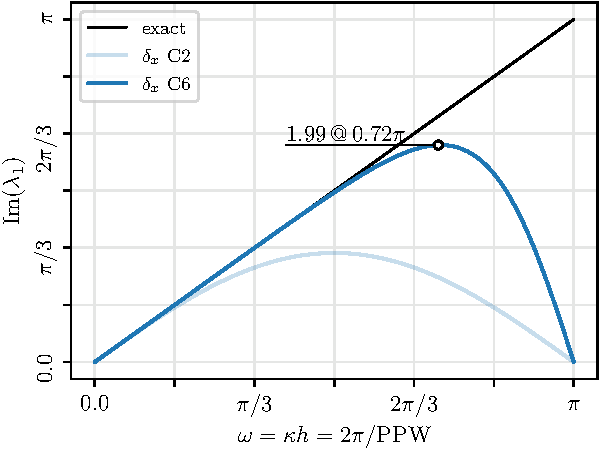
\includegraphics[clip,width=0.49\textwidth]{figs/fdm1}\hfill
  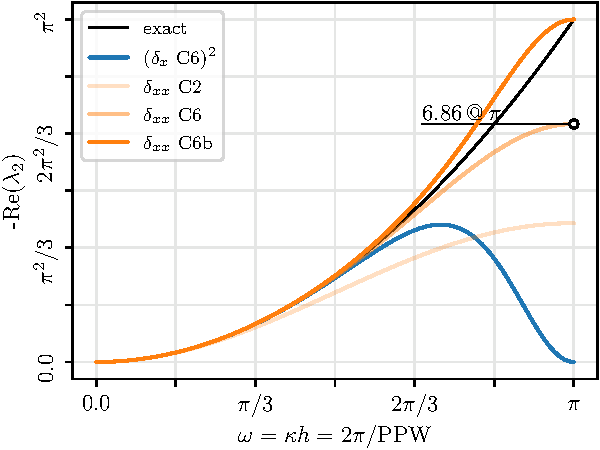
\includegraphics[clip,width=0.49\textwidth]{figs/fdm2}
  \caption{Modified wavenumbers of the FDM approximations to the (left) first-order derivative and (right) second-order derivatives. The blue line in right panel corresponds to the operator $\delta_{x}\delta_{x} =(A_1^{-1}B_1)^2$. The interval $[-\pi,0$ is simply the anti-symmetric extension in the left panel, and the symmetric extension in the right panel. The scheme compact a corresponds to the 5-point stencil in \cite{Lele:1992} and compact b corresponds to the 7-point stencil in \cite{Lamballais:2011}. The latter is the default scheme in the code.}
  \label{fig:fdm}
\end{figure}

It is also useful to use the notation
\begin{equation}
  \hat{\mathbf{s}} = W\, \mathbf{s}\,\qquad \mathbf{s}=W^{-1}\hat{\mathbf{s}}\;.
\end{equation}
for the discrete Fourier transform (DFT) defined by equation~(\ref{equ:dft}),
where $W$ is the DFT matrix. Let us consider the first-order derivative in
equation~(\ref{equ:fdm}). Then, we can write
\begin{equation}
  \hat{\mathbf{s'}}=W\, \mathbf{s'} =
  [(1/h)W(A_1^{-1}B_1)W^{-1})W\mathbf{s} = (1/h)\Lambda_1\hat{\mathbf{s}} \;.
\end{equation}
From this relation between the vectors $\hat{\mathbf{s'}}$ and $\hat{\mathbf{s}}$ and equation~(\ref{equ:lambda}), we deduce that the array $\Lambda_1$ is diagonal with $\{\lambda_k\}_0^{n-1}$ as diagonal elements. Moreover, since $W$ is invertible, $W$ represents just a similarity transformation -- a change of base -- and therefore we know that the matrices $A_1^{-1}B_1$ and $\Lambda_1$ have the same eigenvalues. Hence, $\{\lambda_k\}_0^{n-1}$ is simply the set of eigenvalues of $A_1^{-1}B_1$; figure~\ref{fig:fdm} shows the curve through the imaginary part of half of them. In the complex plane, the numbers $\{\lambda_{1,k}\}_0^{n-1}$ corresponding to the first-order derivative move in the imaginary axis, and the numbers $\{\lambda_{2,k}\}_0^{n-1}$ corresponding to the second-order derivative move in the negative part of the real axis.
%This exercise might not be relevant for the periodic case because we can obtain $\{\lambda_k\}_0^{n-1}$ easily by substituting equation~(\ref{equ:dft}) into equation~(\ref{equ:coefs}), but it is clarifying for the non-periodic cases because the equivalent of figure~\ref{fig:fdm} is simply the spectrum of $A_1^{-1}B_1$, in general, a set of points in the complex plane.

We can calculate the FD approximation to the second-order derivative as $\delta_{x}\delta_{x} \mathbf{s} = (A_1^{-1}B_1)^2$, that is, to consecutively apply the FD approximation to the first-order derivative twice. However, the spectral transfer function of the FD operator $\delta_{x}\delta_{x}$ falls to zero at the Nyquist frequency, as shown in figure~\ref{fig:fdm}, which results in a very poor representation of the diffusion terms at the high wavenumbers. This property can become very important because the errors derived from the aliasing in calculating the non-linear terms accumulate and the use of filter might become unavoidable to have stable simulations. Hence, we use a direct discretization of the second-order derivative operator, compact a or compact b.

Last, a uniform grid $\{x_j=x_1+(j-1)h:\, j = 1,\ldots,n\}$ has been considered so far. If a non-uniform grid $\{x_j:\, j = 1,\ldots,n\}$ is employed instead, we can define $\mathbf{x'} = (1/h)A_1^{-1}B_1\mathbf{x}$ from the mapping between the computational and the physical domains and the calculation of the approximation $\delta_{x} \mathbf{s}$ to the first-order derivative is given by
\begin{equation}\label{equ:nonuniform1}
  (A_1D_1)\, \delta_x \mathbf{s}=(1/h)B_1 \mathbf{s} \;,
\end{equation}
that is, $A_1$ should be replaced by $A_1D_1$, where $D_1=\text{diag} (\mathbf{x'})$ is a diagonal matrix with $\{x'_j\}$ as diagonal elements. Similarly, for the FD approximation to the second-order derivative, we obtain
\begin{equation}
  (A_2D_1^2)\, \delta_{xx} \mathbf{s}=(1/h^2)B_2 \mathbf{s} - (A_2D_2)\,\delta_x
  \mathbf{s} \;,
\end{equation}
where $D_2=\text{diag} (\mathbf{x''})$ is again a diagonal matrix with
$\{x''_j\}$ as diagonal elements; these elements are the components of the vector $\mathbf{x''} = (1/h^2)A_2^{-1}B_2\mathbf{x}$. As a result of using this Jacobian formulation for non-uniform grids, we need to calculate the approximation to the first-order derivative in order to calculate $\delta_{xx} \mathbf{s}$. In general, that is not a problem because we need both, the first- and the second-order derivatives, in all the transport equations.

We could reformulate the calculation of the second-order derivative as
\begin{subequations}\label{equ:nonuniform2}
  \begin{align}
    (A_2D_1^2)\, \mathbf{s}^*&=(1/h^2)B_2 \mathbf{s} \;,\\
    \delta_{xx} \mathbf{s}&= \mathbf{s}^*- (D_1^{-2}D_2)\,\delta_x  \mathbf{s} \;,
  \end{align}
\end{subequations}
where $D_1^{-2}D_2$ is a diagonal matrix and could be precomputed. This formulation is clearer and useful for the stability analysis, but not faster.

A direct formulation of compact FD approximation to the second-order derivative for non-uniform grids is needed, however, when using the implicit temporal scheme for the diffusion terms in order to solve exactly the corresponding Helmholtz equations, without any approximation. Such a direct formulation leads to the system form~(\ref{equ:fdm}). We followed \cite{Shukla:2005}.

\subsection{Advection and Diffusion}

The non-linear advection terms can be formulated in conservative, convective and skew-symmetric forms \citep{Blaisdell:1996,Kravchenko:1997}. The molecular transport terms can be formulated in the conservative and non-conservative forms (this latter if transport coefficients are constant).

In the convective formulation, the routines {\tt OPR\_BURGERS\_*} combine the first and second-order derivative operators as
\begin{equation}
f=\epsilon s'' - u s'\;
\end{equation}
where $s$ is a scalar field, $u$ a velocity field, and $\epsilon$ is the diffusivity. The combination reduces transpositions, either locally or across processors. The reason is that, in general, we need 2 transpositions for $s''$, forward and backward, and similarly for $s'$, which amounts to 4 transpositions. In the the combined form, we need 1 forward transposition for $s$ and 1 for $u$, and then 1 backward transposition for the result $f$. In total, 3 transpositions. The addition and multiplication operations are done in transposed space. If $u= s$, then it is only 2 transpositions that we need. When $u\ne s$, then the transposed velocity needs to be passed through the arguments in case it is needed.

In the anelastic mode, the operator calculates
\begin{equation}
f=\rho_\mathrm{bg}^{-1}\epsilon s'' - u s'\;,
\end{equation}
where $\rho_\mathrm{bg}$ is the background density profile.

We could reformulate the calculation of $\mathbf{f}$ by combining the linear operation with the calculation of the second derivative, which yields
\begin{equation}
    \epsilon^{-1}(A_2D_1^2)\, \mathbf{f}=(1/h)B_2 \mathbf{s}
    - A_2(D_2 + \epsilon^{-1}D_1^2\mathbf{u})\,\delta_x  \mathbf{s} \;,
\end{equation}
or
\begin{subequations}
  \begin{align}
    \epsilon^{-1}(A_2D_1^2)\, \mathbf{f}^*&=(1/h)B_2 \mathbf{s} \;,\\
    \mathbf{f}&= \mathbf{f}^*- (\epsilon D_1^{-2}D_2 + \mathbf{u})\,\delta_x  \mathbf{s} \;,
  \end{align}
\end{subequations}
where $\epsilon D_1^{-2}D_2$ is a diagonal matrix and could be precomputed. This formulation is clearer, but not sure if faster, and we need more memory because $\epsilon D_1^{-2}D_2$ varies with $\epsilon$.

\subsection{Filters}\label{sec:filters}

See file {\tt operators/opr\_filter}. The kernels of the specific algorithms are in the library {\tt filters}. Used in previous versions for long-term stability, filters are now mainly used for post-processing.

There are global filters and directional filters. Global filters are spectral filters in the horizontal plane, and Helmholtz-based filters. Band spectral filters remove the energy content outside a band $[\alpha_1,\alpha_2]$ in frequency space. Erf spectral filters are low- and high-pass filters defined at $\alpha_1$ with a thickness $\alpha_2$ in the logarithm of the frequency ($\alpha_1>0$ for high-pass filter, and $\alpha_1<0$ for low-pass filter). Helmholtz-based filters are defined by
\begin{equation}
  (1-\alpha^2\nabla^2) f = s \;,
\end{equation}
where $s$ is the original field, $f$ is the filtered field, and $\alpha=\lambda/(2\pi)$ where $\lambda$ is the filter size. This equation is transformed into the Helmholtz equation and solved as explained in section~\ref{sec:helmholtz}. This filter is motivated by the Navier-Stokes-alpha model \citep{Foias:2001}. Along the vertical non-periodic direction, we can impose Dirichlet or Neumann boundary conditions, where the former option maintains the value of the field at the boundary and the latter option imposes a zero gradient.

Directional filters are a sequence of one-dimensional filters in each direction. There are compact filters, which are implemented following \cite{Lele:1992}, and top-hat filters (or box filter), which are implemented using the trapezoidal rule to discretize the integral.

As an example of top-hat filter, let us consider a top-hat filter of a function $s(x)$ where the filter size is four times the grid size. Then, the value at the grid node $x_i$ of the filtered function $f(x)$ is
\begin{equation}
  f_i = \frac{1}{\Delta_{f,i}}\left\{\frac{s_{i-2}+s_{i-1}}{2}\Delta_{i-2}+
  \frac{s_{i-1}+s_{i}}{2}\Delta_{i-1}+\frac{s_{i}+s_{i+1}}{2}\Delta_{i}+
  \frac{s_{i+1}+s_{i+2}}{2}\Delta_{i+1}\right\}
\end{equation}
where
\begin{subequations}
  \begin{align}
    \Delta_i&=x_{i+1}-x_{i} \;,\\
    \Delta_{f,i}&=x_{i+2}-x_{i-2}=\Delta_{i-2}+\Delta_{i-1}+\Delta_{i}+\Delta_{i+1} \;.
  \end{align}
\end{subequations}
The linear operation can be written as
\begin{equation}
  f_i = c_{1,i}s_{i-2}+c_{2,i}s_{i-1}+c_{3,i}s_{i}+c_{4,i}s_{i+1}+c_{5,i}s_{i+2} \;,
\end{equation}
where the coefficients are
\begin{subequations}
  \begin{align}
    c_{1,i} &= (2\Delta_{f,i})^{-1} \Delta_{i-2}\;,\\
    c_{2,i} &= (2\Delta_{f,i})^{-1}(\Delta_{i-1}+\Delta_{i-2})\;,\\
    c_{3,i} &= (2\Delta_{f,i})^{-1}(\Delta_{i}+\Delta_{i-1})\;,\\
    c_{4,i} &= (2\Delta_{f,i})^{-1}(\Delta_{i+1}+\Delta_{i})\;,\\
    c_{5,i} &= (2\Delta_{f,i})^{-1}\Delta_{i+1}\;.
    \end{align}
\end{subequations}
For the tophat filter, we can imposed free or solid boundary conditions along the non-periodic directions. The former option uses ghost cells where the function is the linear extrapolation of $s(x)$ based on the values at the two nodes next to the boundary. The latter option uses ghost cells where the function is constant and equal to the boundary value of $s(x)$. As an example, consider the solid boundary near $i=1$ for the example above:
\begin{subequations}
  \begin{align}
    f_1 &= \tilde{c}_{3,1}s_{1}+c_{4,1}s_{2}+c_{5,1}s_{3} \;,\\
    f_2 &= \tilde{c}_{2,2}s_{1}+c_{3,2}s_{2}+c_{4,2}s_{3}+c_{5,2}s_{4} \;,
  \end{align}
\end{subequations}
where the coefficients are
\begin{subequations}
  \begin{align}
    i=1\;:\quad\tilde{c}_{3,1} &= c_{1,1}+c_{2,1}+c_{3,1} =(2\Delta_{f,1})^{-1}5\Delta_{1}
    =(2\Delta_{f,i})^{-1}[2(n-i)+3]\Delta_{1}\;,\\
    i=2\;:\quad\tilde{c}_{2,2} &= c_{1,2}+c_{2,2}\phantom{(+c_{3,1}} =(2\Delta_{f,2})^{-1}3\Delta_{1}
    =(2\Delta_{f,i})^{-1}[2(n-i)+3]\Delta_{1}\;,
  \end{align}
\end{subequations}
together with
\begin{subequations}
  \begin{align}
    i=1\;:\quad\Delta_{f,1}&=3\Delta_{1}+\Delta_{2}\phantom{+\Delta_{3})}=
    (n-i+2)\Delta_{1}+\ldots+\Delta_{n+i-1}\;,\\
    i=2\;:\quad\Delta_{f,2}&=2\Delta_{1}+\Delta_{2}+\Delta_{3}=
    (n-i+2)\Delta_{1}+\ldots+\Delta_{n+i-1}\;,
  \end{align}
\end{subequations}
Generalizing to a filter halfsize $n$, we obtain:
\begin{subequations}
  \begin{align}
    i=1,\ldots,n\;:\quad
    & \Delta_{f,i} = (n-i+1)\Delta_{1}+\sum_{k=1}^{n+i-1}\Delta_{k} \;,\\
    & i_\mathrm{org}=n-i+1\;,\\
    &\tilde{c}_{i_\mathrm{org}+1,i} = (2\Delta_{f,i})^{-1}[2(n-i+1)+1]\Delta_{1}\;,\\
    &f_{i} =\tilde{c}_{i_\mathrm{org}+1,i}\,s_1+\sum_{k=2}^{n+i} c_{i_\mathrm{org}+k,i}\,s_{k} \;.
  \end{align}
\end{subequations}
Near the boundary $i=i_\mathrm{max}$, we obtain:
\begin{subequations}
  \begin{align}
    i=i_\mathrm{max}-n+1,\ldots,i_\mathrm{max}\;:\quad
    & \Delta_{f,i} = \sum_{k=i-n}^{i_\mathrm{max}-1}\Delta_{k} +(n+i-i_\mathrm{max})\Delta_{i_\mathrm{max}-1}\;,\\
    & i_\mathrm{org}=n-i+1\;,\\
    &\tilde{c}_{i_\mathrm{org}+i_\mathrm{max},i} = (2\Delta_{f,i})^{-1}[2(n+i-i_\mathrm{max})+1]\Delta_{i_\mathrm{max}-1}\;,\\
    &f_{i} =\sum_{k=i-n}^{i_\mathrm{max}-1} c_{i_\mathrm{org}+k,i}\,s_{k}+\tilde{c}_{i_\mathrm{org}+i_\mathrm{max},i}\,s_{i_\mathrm{max}} \;.
  \end{align}
\end{subequations}

In any case, the algorithm can be expressed formally as a matrix multiplication, the diagonals being calculated once in the initialization step and being stored in the filter-structure data.

\subsection{Fourier transform}

See file {\tt operators/opr\_fourier}. It is based on the FFTW library and it has been already discussed in the previous section (see text around equation~({\ref{equ:dft})).It is used in the pre-processing (generation of the   initial random field), in the post-processing (spectral analysis), and also during the simulation (Poisson and Helmholtz solvers).

The Fourier transform is applied by default to an array {\tt imax\_total}$\times${\tt(jmax\_total+2)}$\times${\tt kmax\_total}. The reason to add two additional planes {\tt \{jmax\_total+1,jmax\_total+2\}} is that we need them for the boundary conditions of the Poisson equations, and we make that the standard procedure. If not needed, then these two planes contain simply zeros.

The sequence of transformations is $Ox\rightarrow Oz\rightarrow Oy$. The transformed field contains the Nyquist frequency, so it needs an array {\tt(imax\_total/2+1)}$\times${\tt(jmax\_total+2)}$\times${\tt kmax\_total} of complex numbers.

Given the scalar field $s$, the power spectral density $\{E_0,\,E_1,\,\ldots,\,E_{N/2}\}$ is normalized such that
\begin{equation}
\langle s^2\rangle = E_0+2\sum_0^{N/2-1}E_n+E_{N/2} \;.
\end{equation}
The mean value is typically removed, such that the left-hand side is $s^2_\text{rms}$. The Nyquist frequency energy content $E_{N/2}$ is not written to disk, only the $N/2$ values $\{E_0,\,E_1,\,\ldots,\,E_{N/2-1}\}$.

\subsection{Poisson equation}

See file {\tt operators/opr\_poisson}. Given the scalar field $s$, obtain the scalar field $f$ such that
\begin{equation}
  \nabla^2 f= s \;,
\end{equation}
complemented with appropriate boundary conditions.  The current version only handles cases with periodic boundary conditions along $Ox$ and $Oz$. It performs a Fourier decomposition along these two directions, to obtain the a set of finite difference equations along $Oy$ of the form
\begin{equation}
  \delta_x \delta_x \mathbf{f}|_j - (\lambda_1/h)^2\mathbf{f}|_j=\mathbf{s}|_j
  \;,\qquad j=2,\ldots,n-1 \;,
\end{equation}
$\lambda_1\in\mathbb{R}$, where boundary conditions need to be provided at $j=1$ and $j=n$.  The algorithm is described in \cite{Mellado:2012}. These routines are in the source file {\tt dns/opr\_fde\_pool}.

\subsection{Helmholtz equation}
\label{sec:helmholtz}

See file {\tt operators/opr\_helmholtz}. Given the scalar field $s$, obtain the scalar field $f$ such that
\begin{equation}
\nabla^2 f + \alpha f= s \;,
\end{equation}
complemented with appropriate boundary conditions. The current version only handles cases with periodic boundary conditions along $Ox$ and $Oz$. The algorithm is similar to that used for the Poisson equation. It performs a Fourier decomposition along these two directions, to obtain the a set of finite difference equations along $Oy$ of the form
\begin{equation}
  \delta_x \delta_x \mathbf{f}|_j - (\lambda_2/h^2-\alpha)\mathbf{f}|_j=\mathbf{s}|_j
  \;,\qquad j=2,\ldots,n-1 \;,
\end{equation}
$\lambda_2\in\mathbb{R}$, where boundary conditions need to be provided at $j=1$ and $j=n$. The difference is that, for the Helmholtz equation, we also include the case in which the second-order derivative is implemented in terms of the $\delta_{xx}$ FDM operator, not only the $\delta_x\delta_x$ FDM operator.

%%%%%%%%%%%%%%%%%%%%%%%%%%%%%%%%%%%%%%%%%%%%%%%%%%%%%%%%%%%%%%%%%%%%%%%%%%%%%%%%
%%%%%%%%%%%%%%%%%%%%%%%%%%%%%%%%%%%%%%%%%%%%%%%%%%%%%%%%%%%%%%%%%%%%%%%%%%%%%%%%
\section{Time marching schemes}

See file {\tt tools/dns/time\_rungekutta}. The time advancement is based on
Runge-Kutta methods (RKM).

\subsection{Explicit schemes}

We can use three- or five-stages, low-storage RKM that gives third- or fourth-order accurate temporal integration, respectively \citep{Williamson:1980,Carpenter:1994}. The essential feature is that only two levels are needed at a time, reducing thereby the number of three-dimensional arrays compared to the convectional Runge-Kutta schemes. In particular, the implementation is
\begin{align*}
  &\mathbf{h} = 0 \\
  &\left.
  \begin{array}{rrl}
    \mathbf{h} \leftarrow   & \mathbf{h} &+ \mathbf{f}(\mathbf{s},t+C_M\tau) \\
    \mathbf{s}\, \leftarrow & \mathbf{s} &+ B_M\tau\;\mathbf{h}       \\
    \mathbf{h} \leftarrow   &A_M\; \mathbf{h}& \\
  \end{array}
  \right] M \textrm{ times},\\
\end{align*}
where $M=3$ or $M=5$, $C_1=0$ and we do not need the last step for the last stage.  The stability properties for the biased finite difference schemes are considered in \cite{Carpenter:1993}. The incompressible formulation follows \cite{Wilson:1998}.

The analysis of time marching schemes is based on the linearization of of the right-hand size~(\ref{equ:problem}), and its diagonalization to obtain a set of ODEs of the form
\begin{equation}
  \frac{ds_j}{dt}=\lambda_j s_j \;,
\end{equation}
where $s_j$ can be a complex function of the real variable $t$, and $\lambda_j$ is the corresponding eigenvalue, a complex number. Given the initial condition $s^n$ at $t_n$, the RKM provides an approximation $s^{n+1}$ to $s(t_{n+1})$, where the time step is $\tau=t_{n+1}-t_n$. The ratio provides the amplification factor $r=s^{n+1}/s^n$. The exact amplification factor is $\exp(\lambda \tau)$, whereas that from the discrete method is
\begin{equation}
  r=1+\sum_1^pc_k(\lambda \tau)^k\;,
\end{equation}
the coefficients depending on the RKM method and $p$ being the number of stages. The region of absolute stability is the region of the complex plane $\lambda\tau$ for which $|r|<1$. In addition, we can compare the approximation with the exact value
\begin{equation}
  \rho\exp(i\theta)=\frac{r}{\exp(\lambda\tau)}\;,
  \label{equ:rkmerror}
\end{equation}
such that $\rho-1$ and $\theta$ represents the amplitude (or dissipation) error and the phase (or dispersion) error, respectively \citep{Hu:1996}.

\begin{figure}[!ht]
  \centering
  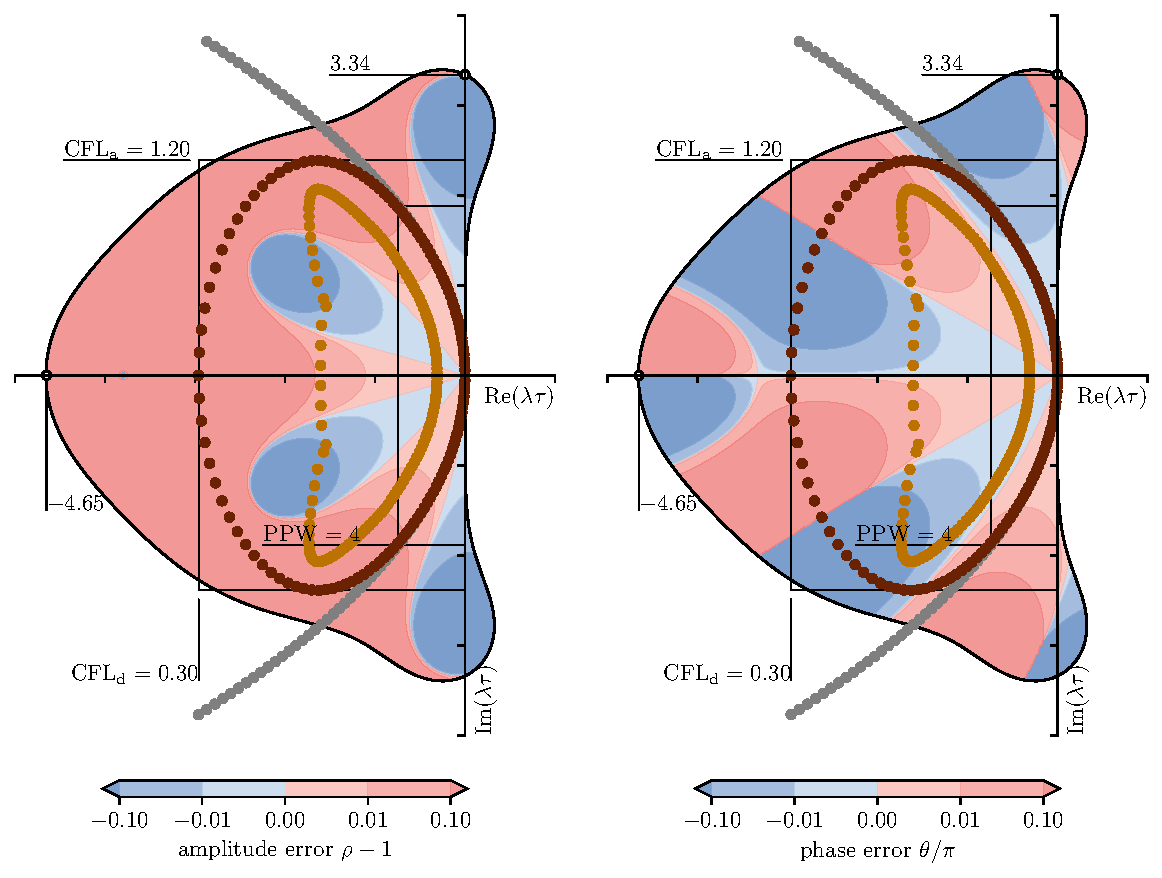
\includegraphics[clip,height=0.7\textwidth]{figs/rkm4}
  \caption{Fourth-order explicit Runge-Kutta scheme. Colored area indicates the stability region. The five zeros of the polynomial $r=r(\lambda\tau)$ are enclosed by the blue closed regions in the left panel. Markers indicate the eigenvalues for the advection-diffusion equation and $n=128$: gray, periodic case with spectral FDMs; dark brown, periodic case with compact FDMs; light brown, Dirichlet case with compact FDMs.}
  \label{fig:rkm}
\end{figure}

For the fourth-order five-step Runge-Kutta method that we use in the code, one finds (see figure~\ref{fig:rkm})
\begin{equation}
  r=1+\sum_1^4\frac{1}{k!}(\lambda \tau)^k+\frac{1}{200}(\lambda \tau)^5 \;.
\end{equation}
The equation above shows the forth-order accuracy, since the first term that deviates from the Taylor series of the exponential function is proportional to $(\lambda\tau)^5$. The crossing points of the boundary of the stability region with the real and imaginary axis are $(\lambda \tau)_{r}\simeq-4.65$ and $(\lambda \tau)_{i}\simeq\pm 3.34$. These numbers determine the maximum CFL numbers associated with the advection-diffusion equation, which is the basis for many non-reacting flows (a source term might add an additional stability constraint for). Assuming periodic boundary conditions for simplicity, we can diagonalize the original system to the set of equations
\begin{equation}
  \frac{d\hat{s}_j}{dt}=(ic\lambda_{1,j}/h -\nu\lambda_{2,j}/h^2)\hat{s}_j \;,\qquad j=0,\ldots,n-1\;,
  \label{equ:eigenvalues}
\end{equation}
according to the eigenvalue analysis discussed in section~\ref{sec:fdm}. In the expression above, $c$ is a constant representing an advection velocity and $\nu$ is the viscosity.  The expression within parenthesis is the eigenvalue $\lambda_j$ and it needs to belong to the stability region shown for the algorithm to be stable. This condition implies
\begin{equation}
  \frac{\nu\tau}{h^2}<\frac{|(\lambda \tau)_{r}|}{\max_j\{\lambda_{2,j}\}}\;,\qquad
  \frac{c\tau}{h}<\frac{|(\lambda \tau)_{i}|}{\max_j\{\lambda_{1,j}\}} \;.
\end{equation}
The left-hand sides in the expressions above are the $\textrm{CFL}$ numbers $\textrm{CFL}_\mathrm{d}$ and $\textrm{CFL}_\mathrm{a}$ for the diffusion and the advection operators, respectively. The right-hand sides provide the upper bounds $\textrm{CFL}_\mathrm{d,max}=4.65/6.86=0.68$ ($4.65/\pi^2=0.47$ if we use \cite{Lamballais:2011}) and $\textrm{CFL}_\mathrm{a,max}=3.34/1.99=1.68$ having used for $\max_j\{\lambda_{2,j}\}$ and $\max_j\{\lambda_{1,j}\}$ the values shown in figure~\ref{fig:fdm}.

Besides stability, we also want a small error. Figure~\ref{fig:rkm} shows the amplitude and phase errors as defined in (\ref{equ:rkmerror}). That figure explains the reason to use CFL numbers that are smaller than the maximum for stability. The value $\mathrm{CFL}_\mathrm{a}=0.7\,\mathrm{CFL}_\mathrm{a,max}\simeq 1.2$ is used in the code by default. In the real axis, the code uses by default $1/4$ of the limit in the imaginary axis, that is, $\textrm{CFL}_\mathrm{d}=0.3$. Wavenumbers corresponding to more than 4 PPW fall approximately within 10\% error.

For the third-order Runge-Kutta method that we use in the code, one finds (see figure~\ref{fig:rkm3})
\begin{equation}
  r=1+\sum_1^3\frac{1}{k!}(\lambda \tau)^k \;.
\end{equation}
The maximum $\mathrm{CFL}$ numbers to guarantee stability for the advection and diffusion operators are $\mathrm{CFL}_\mathrm{a,max} = 1.73/1.989=0.871$ and $\mathrm{CFL}_\mathrm{d,max} = 2.57/6.857=0.375$ ($2.57/\pi^2=0.26$ if we use \cite{Lamballais:2011}), respectively. The value $\mathrm{CFL}_\mathrm{a}=0.7\,\mathrm{CFL}_\mathrm{a,max}\simeq 0.6$ is used in the code by default. In the real axis, the code uses by default $1/4$ of the limit in the imaginary axis, that is, $\textrm{CFL}_\mathrm{d}=0.15$.

\begin{figure}[!ht]
  \centering
  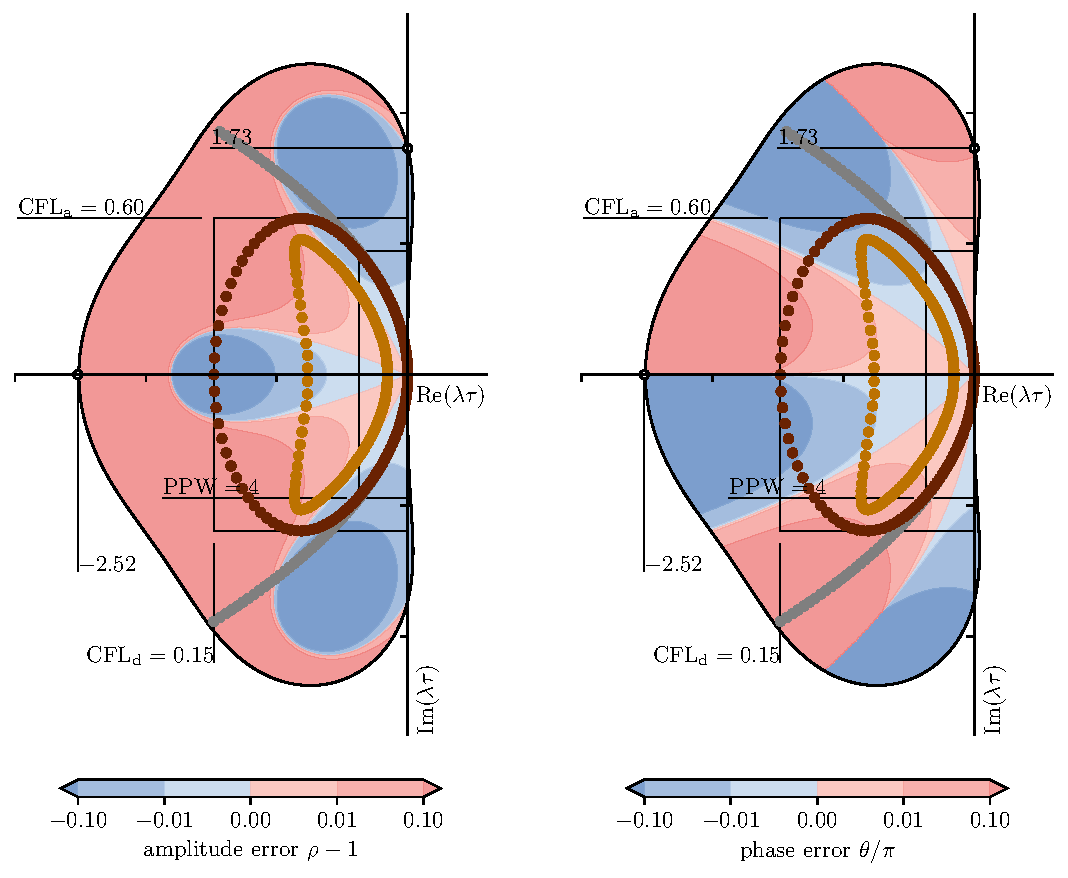
\includegraphics[clip,height=0.7\textwidth]{figs/rkm3}
  \caption{Third-order explicit Runge-Kutta scheme. Colored area indicates the stability region. The five zeros of the polynomial $r=r(\lambda\tau)$ are enclosed by the blue closed regions in the left panel. Markers indicate the eigenvalues for the advection-diffusion equation and $n=128$: gray, periodic case with spectral FDMs; dark brown, periodic case with compact FDMs; light brown, Dirichlet case with compact FDMs.}
  \label{fig:rkm3}
\end{figure}

We have considered the periodic case, which is easier because the eigenvalues can be obtained analytically and both the diffusion and advection operator have the same eigenvectors. For the non-periodic case, we generally need to calculate the eigenvalues numerically.  For instance, let us consider the advection equation inside the domain $[x_1,x_n]$ with a positive advection velocity $u$ and (therefore) the boundary condition imposed at the left boundary $x_1$, that is
\begin{equation}
  \left.\begin{array}{ll}
  d\mathbf{s}/dt|_j = -c\; \delta_x \mathbf{s}|_j & j=2,\ldots,n\\
  s_1=\alpha
  \end{array}\right\} \;,\qquad c\ge 0  \;.
  \label{equ:problem2}
\end{equation}
We know that $\delta_x \mathbf{s} = (1/2)A_1^{-1}B_1\mathbf{s}$, but we only need a relation involving the last $n-1$ components of the vector $\mathbf{s}$, not all of them. This can be obtained by introducing the following block matrices \citep{Lomax:1998,Mellado:2012}
\begin{equation*}
  A_1=
  \left(\begin{array}{cc}a_{11}&\mathbf{a_{12}}^T \\\mathbf{a_{21}}   &A_{22}\\
  \end{array}\right) \;, \qquad
  B_1=
  \left(\begin{array}{cc}b_{11}&\mathbf{b_{12}}^T \\\mathbf{b_{21}}   &B_{22}\\
  \end{array}\right) \;.
\end{equation*}
Then, eliminating $s'_1$ in the original system, yields
\begin{equation}
  hA^R_{22}
  \left(\begin{array}{c}s'_2\\\vdots\\s'_n\end{array}\right) =
  B^R_{22}\left(\begin{array}{c}s_2\\\vdots\\s_n\end{array}\right)+
  s_1\mathbf{b^R_{21}} \;,
\end{equation}
where the $(n-1)\times (n-1)$ matrices $\{A^R_{22}\,,B^R_{22}\}$ and the column vector $\mathbf{b^R_{21}}\in\mathbb{R}^{n-1}$ are
\begin{equation}
  A^R_{22}=A_{22}-\frac{1}{a_{11}}\mathbf{a_{21}}\mathbf{a_{12}}^T \;,\qquad
  B^R_{22}=B_{22}-\frac{1}{a_{11}}\mathbf{a_{21}}\mathbf{b_{12}}^T \;,\qquad
  \mathbf{b^R_{21}}=\mathbf{b_{21}}-\frac{b_{11}}{a_{11}}\mathbf{a_{21}} \;.
\end{equation}
Note that $A^R_{22}$ and $B^R_{22}$ have the same bandwidths as $A$ and $B$, respectively. The element $s'_1$ can be calculated by
\begin{equation}
  s'_1=\frac{1}{ha_{11}}
  \left(\begin{array}{cc}b_{11}\!&\!\mathbf{b_{12}}^T\end{array}\right)
  \mathbf{s} - \frac{1}{a_{11}}
  \mathbf{a_{12}}^T \left(\begin{array}{c}s'_2\\\vdots\\s'_n\end{array}\right)\;.
\end{equation}

% \begin{SCfigure}
% \includegraphics[clip,width=0.45\textwidth]{figs/AdvectionSpectra}
% \caption{Spectra of the matrix $-\{(A^R_{22})^{-1}B^R_{22}\}$ describing the
%   advection operator in problem (\ref{equ:problem2}) for two different problem
%   sizes: black, $n=32$; ref, $n=1024$. As the number of grid points is
%   increased, the role of the boundary conditions decrease and the spectra tends
%   towards that corresponding to periodic boundary conditions, which is purely
%   imaginary (see figure~\ref{fig:fdm}). Note, however, that deviation from the
%   imaginary axis of the eigenvalues is relatively small even for the small size
%   $n=32$, in the context of the dissipation- and dispersion-error regions shown
%   in figure~\ref{fig:rkm}.}\label{fig:advection}
% \end{SCfigure}

Then, the original equation can be written as
\begin{equation}
  \frac{d}{dt}
  \left(\begin{array}{c}s_2\\\vdots\\s_n\end{array}\right) =
  -(c/h)(A^R_{22})^{-1}B^R_{22}\left(\begin{array}{c}s_2\\\vdots\\s_n\end{array}\right)+
  \alpha\mathbf{b^R_{21}} \;,
\end{equation}
so that the set of complex numbers $-(c\tau/h) \textrm{eig} \{(A^R_{22})^{-1}B^R_{22}\}$ have to fall inside the stability region. \citep{Carpenter:1993}.

The same can be done for the diffusion operator. In this case, we impose 2 boundary conditions. If one of the boundary conditions is imposed at $x=x_n$, then we need to eliminate $s_n$ as we have eliminated before $s_1$ when the boundary condition is imposed at $x=x_1$. We obtain now reduced matrices of size $(n-2)\times(n-2)$. For the compact schemes used in the code, this analysis shows that the CFL conditions derived from the spectral FDM approximations are also applicable to the biased schemes used in non-periodic directions, as observed in figure~\ref{fig:rkm}.

%This set of eigenvalues is shown in figure~\ref{fig:advection} for the scheme (35653) used in the code by default, normalized by the prefactor $u\tau/h$. We see that the spectra is dominated by a form relatively close to that of the periodic boundary conditions, which was purely imaginary, and the CFL condition is therefore the same. It happens that some other biased FD formulae at the boundary points can mode part of the spectra into the positive real part of the complex plane, which would lead to unstable algorithms \citep{Carpenter:1993}.

In case of a nonuniform grid, we need to consider the diagonal matrices $D_1$ and $D_2$ in (\ref{equ:nonuniform1}) and (\ref{equ:nonuniform2}). The effect of a varying grid spacing can be studied with the script \texttt{figure.py}. When we use the minimum of grid spacing in the CFL definitions, part of the eigenvalues approach the origin from the stable side.

For the multidimensional case, we need to consider the sum of all possible combinations of eigenvalues in each direction \citep{Lomax:1998}.

\subsection{Implicit schemes}

To be developed. See \cite{Spalart:1991}.

The dissipation and dispersion error maps corresponding to the third-order implicit Runge-Kutta scheme are shown in figure~\ref{fig:rkm3implicit}. The algorithm is unconditionally stable but we need to control accuracy of the diffusion operator for which it is used. The reference value $\textrm{CFL}_d=1.7$ as it gets most of the eigenvalues within the 1\%-error region.

\begin{figure}
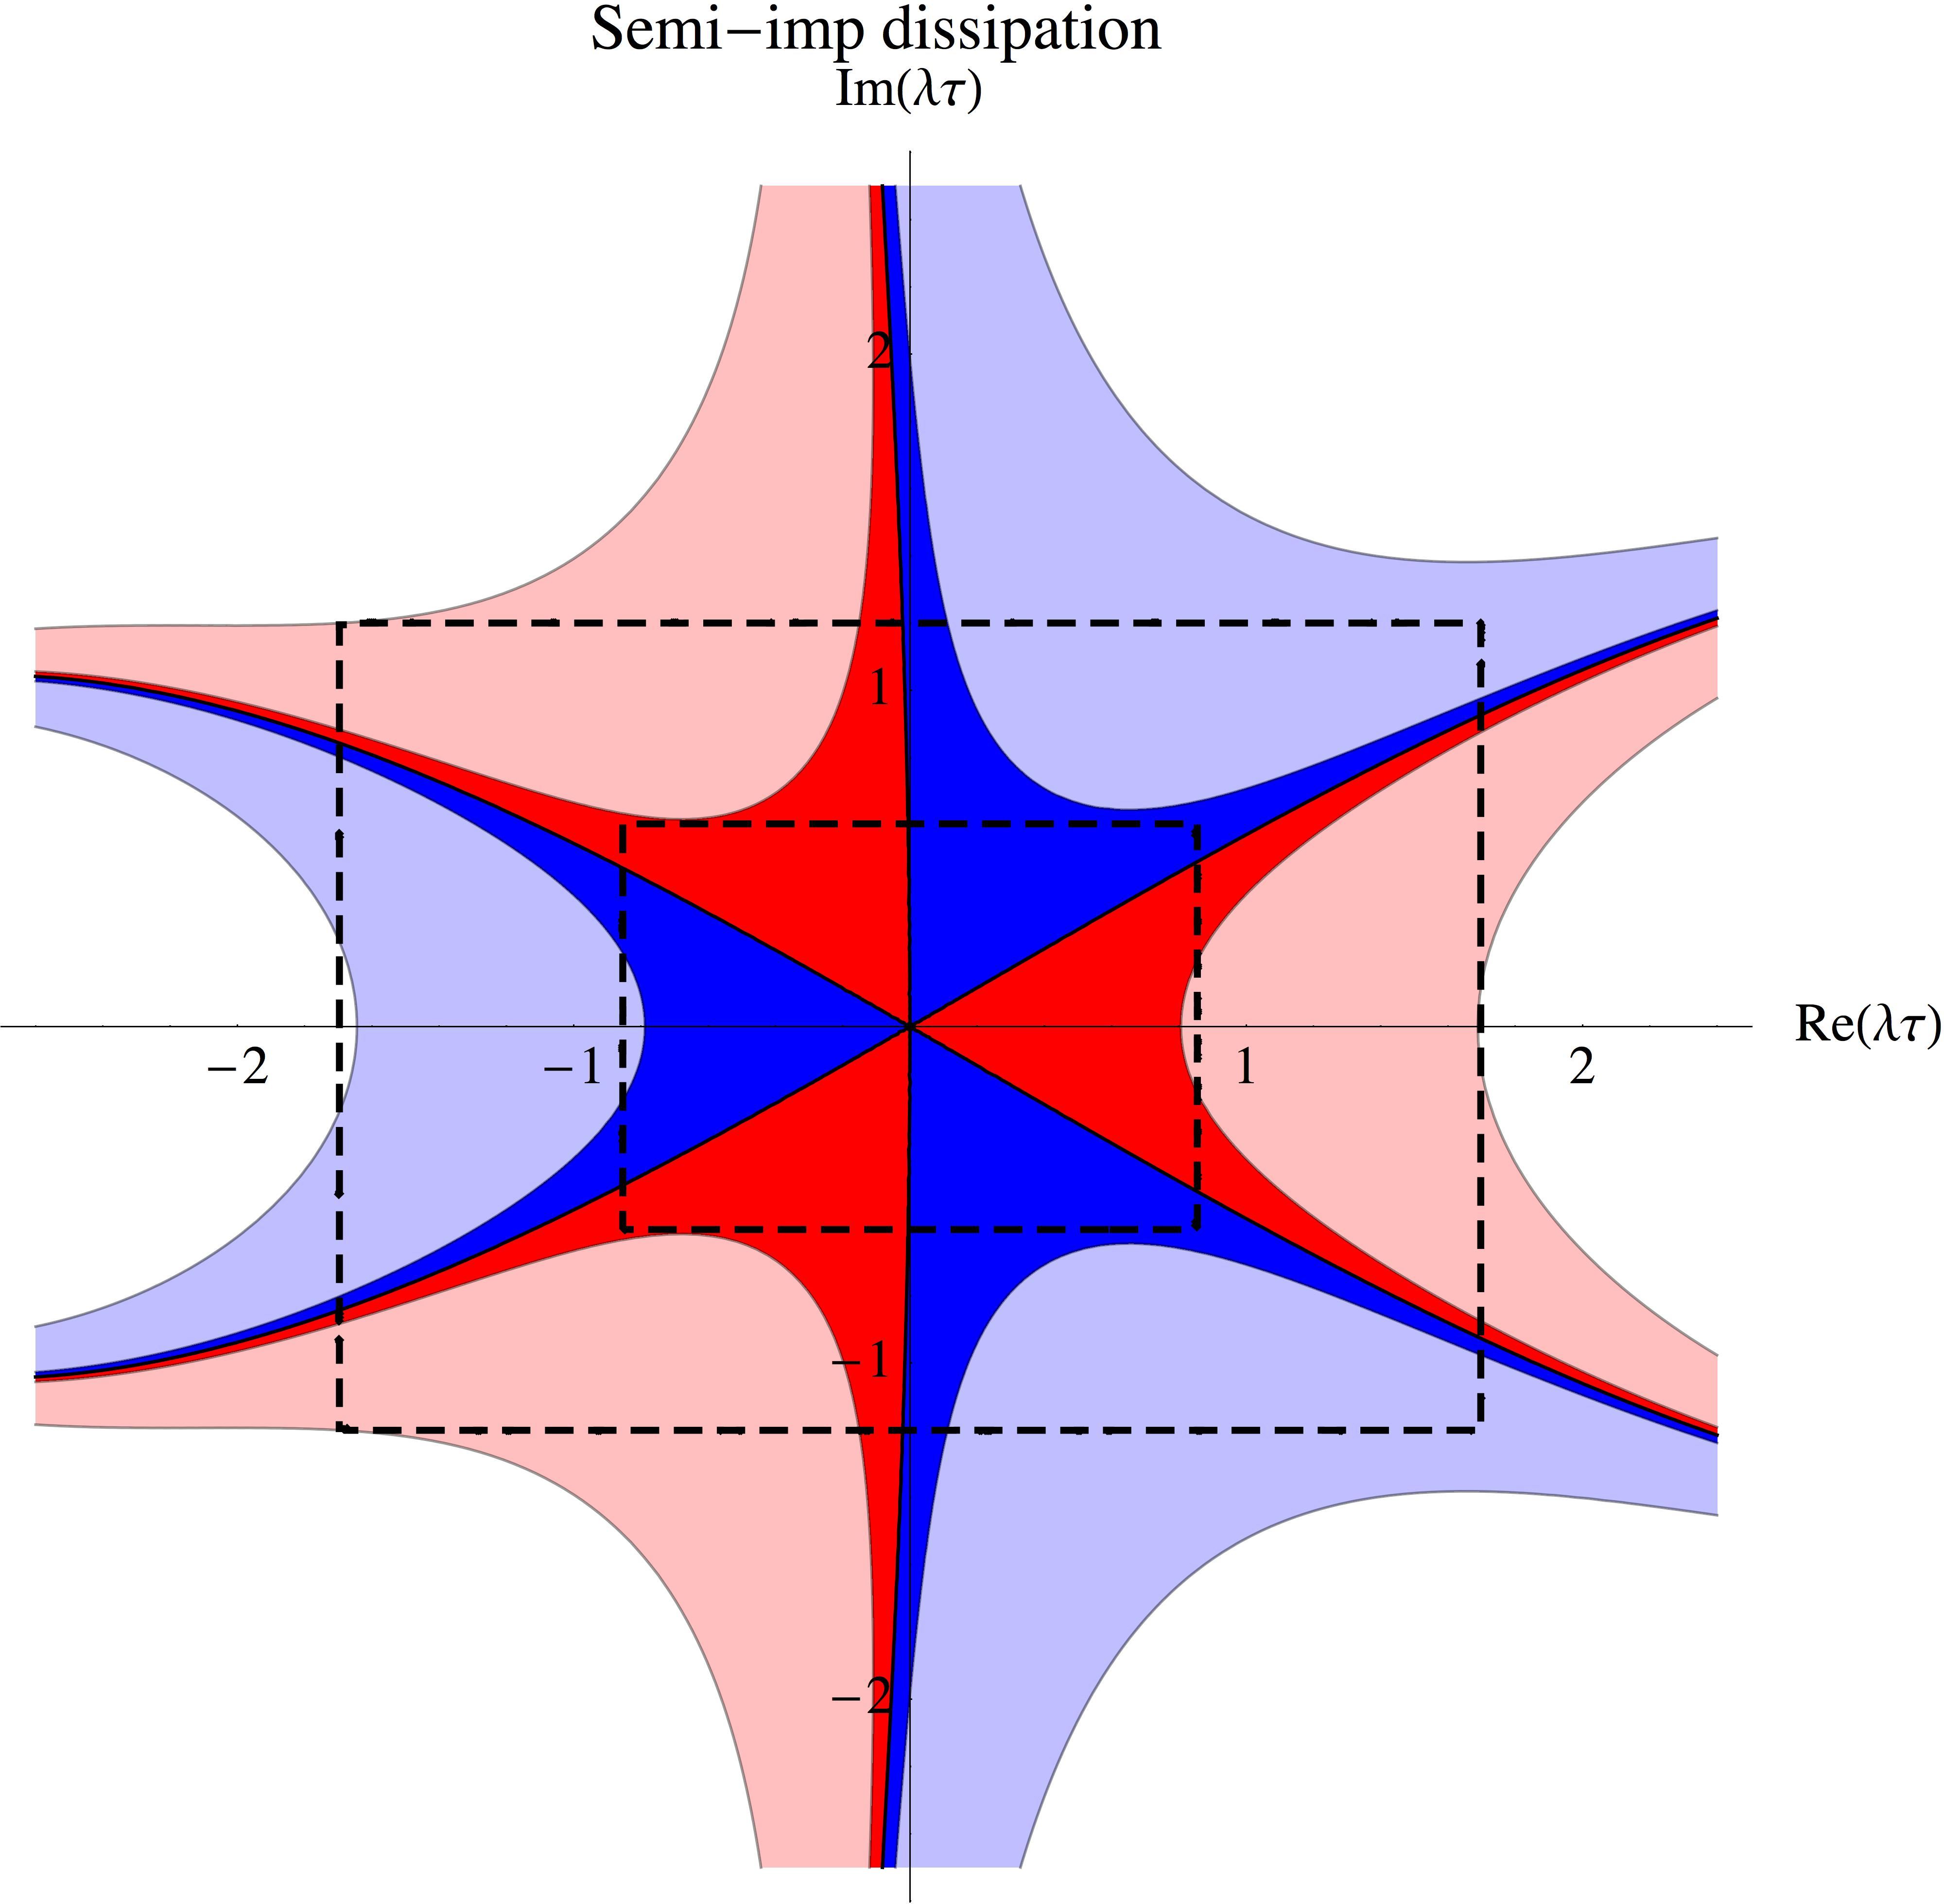
\includegraphics[clip,width=0.49\textwidth]{figs/RK3_imp_diss.jpg}\hfill
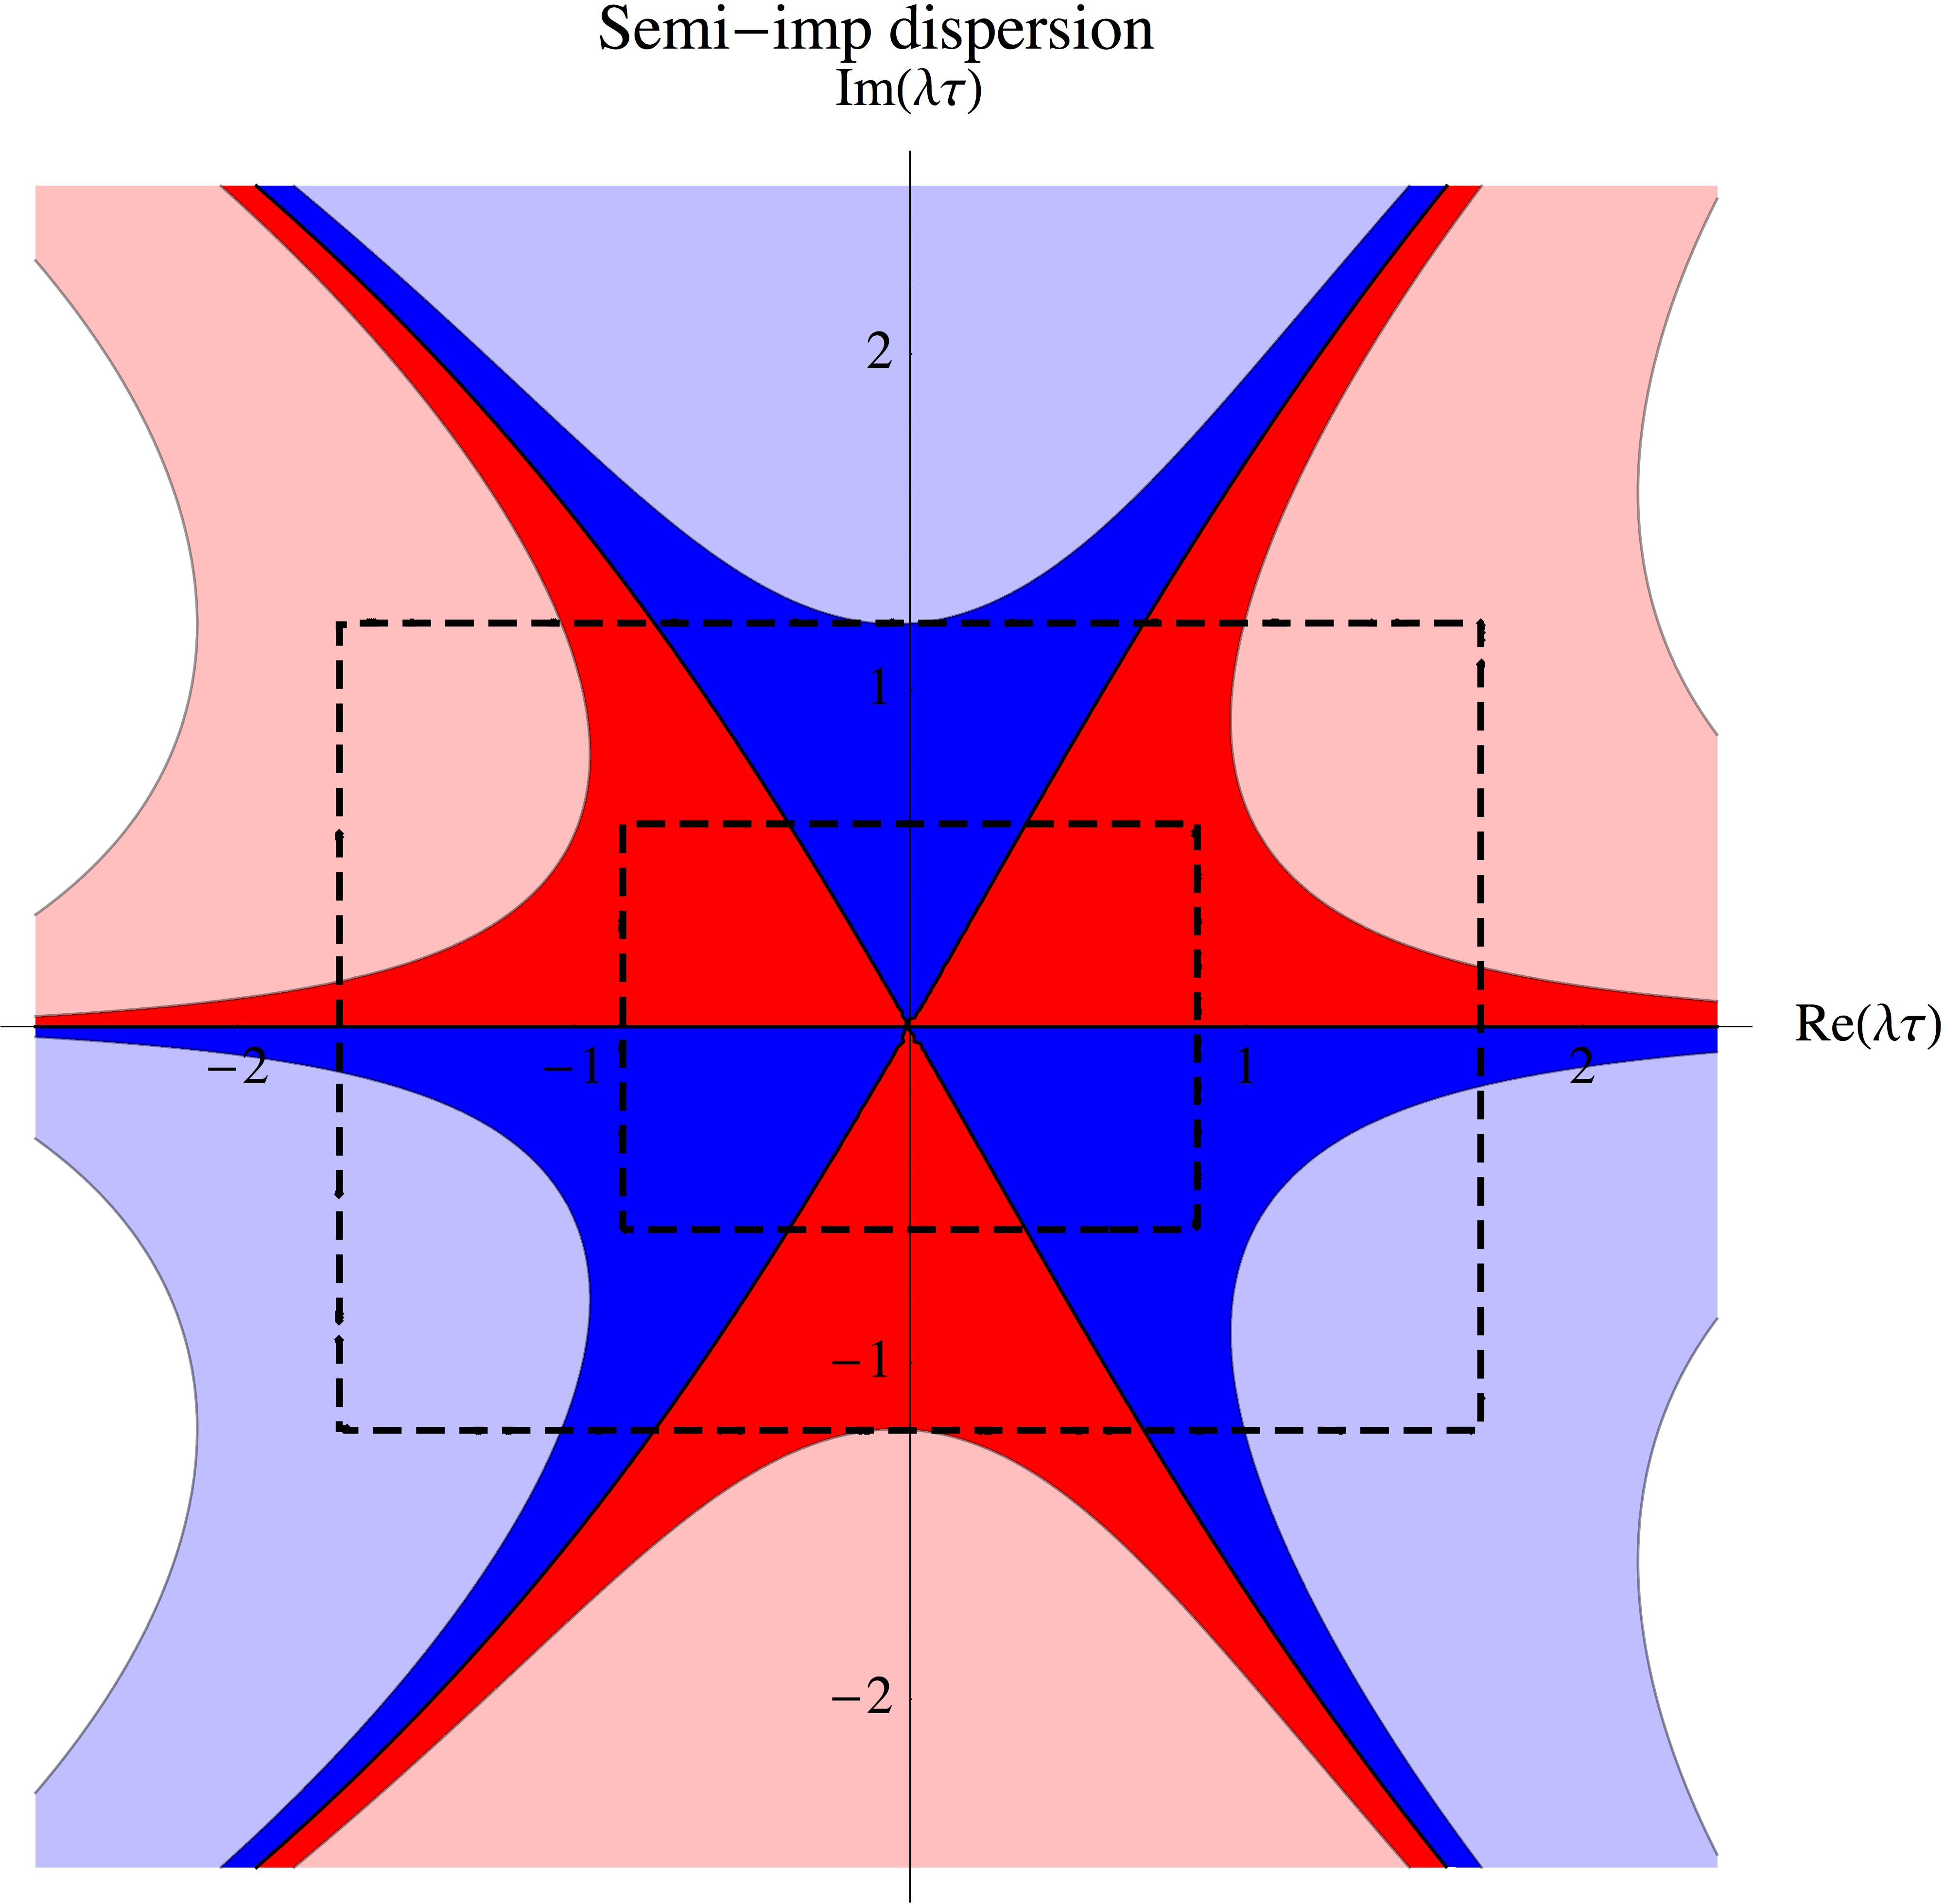
\includegraphics[clip,width=0.49\textwidth]{figs/RK3_imp_disp.jpg}
\caption{Dissipation error (left) associated with the third-order implicit
  Runge-Kutta scheme: dark blue, $0.99<\rho<1$; light blue, $0.90<\rho<0.99$;
  dark red, $1<\rho<1.01$; light red, $1.01<\rho<1.10$. Dispersion error (right)
  associated with the Runge-Kutta scheme: dark blue, $-0.01<\theta/\pi<0$; light
  blue, $-0.10<\theta/\pi<-0.01$; dark red, $0<\theta/\pi<0.01$; light red,
  $0.01<\theta/\pi<0.10$.}\label{fig:rkm3implicit}
\end{figure}

\chapter{Parallelization}\label{sec:mpi}

\section{Domain decomposition}

The domain decomposition is performed along the first and last indexes,
typically $i$ and $k$, respectively, that is, along directions $Ox$ and
$Oz$. Initially, the code only supported 1D decomposition along $Oz$, the
outer-most index. The reason to chose that direction was to simplify I/O and to
maintain homogeneity in the serial part of the algorithm (the largest part) for
the cases with periodicity along that direction (boundary conditions where only
needed in the other two directions, for instance, in a spatially evolving flow
like a jet). When the domain decomposition was extended to a second direction,
we chose $Ox$, the reason being again to keep the algorithm equal in every task
in the cases where homogeneity and periodicity apply along those two
directions. Figure~\ref{fig:parallel01a} sketches this 2D decomposition and
summarizes part of the main code variables. We will use the term MPI task or
simply task (instead of processor, node, core, ...) -- that is, we decompose the
problem into {\tt ims\_npro\_i}$\times${\tt ims\_npro\_k} tasks.  The mapping is
established at read/write time and details follow below. For each task, each
array can be interpreted as {\tt jmax}$\times${\tt kmax} lines of size {\tt
  imax}, as illustrated in figure~\ref{fig:parallel01a}.

\begin{figure}[!ht]
\begin{centering}
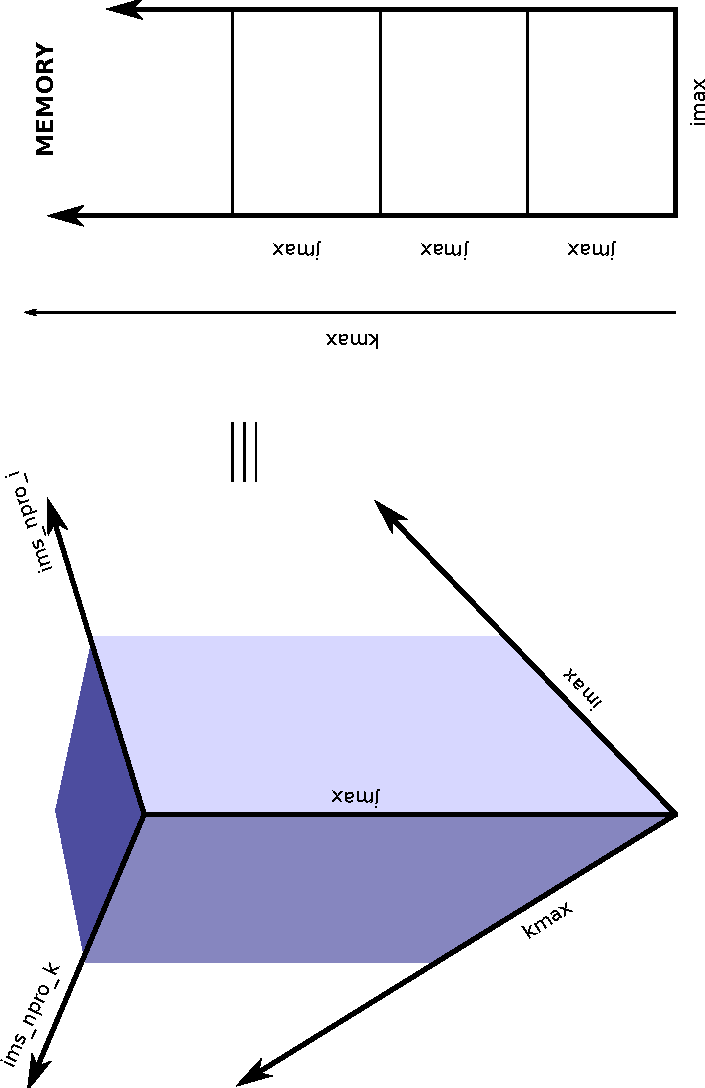
\includegraphics[height=0.8\textwidth,angle=270]{figs/parallel01a}
\caption{Domain decomposition of the global array of size {\tt
    imax\_total}$\times${\tt jmax\_total}$\times${\tt kmax\_total} into the the
  local arrays of size {\tt imax}$\times${\tt jmax}$\times${\tt kmax} using {\tt
  ims\_npro\_i} MPI tasks along the first (inner-most) index and {\tt
  ims\_npro\_k} along the last (outer-most) index. The structure in memory is
  shown in a two-dimensional array where the inner-most index runs up to {\tt
  imax} and the outer-most index runs up to {\tt jmax}$\times${\tt kmax}; it can
  also be interpreted as {\tt kmax} pages of size {\tt imax}$\times${\tt jmax}.}
\label{fig:parallel01a}
\end{centering}
\end{figure}

Two main transpositions are needed to perform the derivatives or any other
implicit operation in which we only need a set of complete lines along the
desired direction contiguously in memory. This is represented in
figure~\ref{fig:parallel01b}. For instance, if we need a derivative along $Ox$
of the field in array $a$, we can interpret the algorithm as follows. Consider
that array as {\tt jmax}$\times${\tt kmax} lines of size {\tt imax}, as
illustrated before in figure~\ref{fig:parallel01a}. Divide {\tt
jmax}$\times${\tt kmax}, the outer index, by {\tt ims\_npro\_i}, so as to have
precisely {\tt ims\_npro\_i} blocks (or colors) of size {\tt imax} times
whatever number you got before. Each of those blocks is send to the
corresponding processor. This operation is masked by creating an appropriate MPI
type, which is done during the initialization of the MPI part of the code. The
constraint we impose is that the ratio {\tt jmax}$\times${\tt kmax}/{\tt
ims\_npro\_i} needs to be an integer -- take this into account when defining the
grid. (This constraint could be avoided using padding, but we do not do it in
these main transposition operations.)

Let us consider now an implicit operation along $Oz$. For this case, each of the
pages {\tt imax}$\times${\tt jmax} needs to be divided by the number of tasks
{\tt ims\_npro\_k}, and this ratio is what needs to be an integer. It is also
seen in figure~\ref{fig:parallel01b} that now we need a stride in the MPI
type. The rest of the transposition algorithm is similar to the previous
case. The code variables containing the corresponding MPI types for the
transposition operations described in the previous and this paragraphs are {\tt
DNS\_MPI\_I\_PARTIAL} and {\tt DNS\_MPI\_K\_PARTIAL}, respectively.

\begin{figure}[!ht]
\begin{centering}
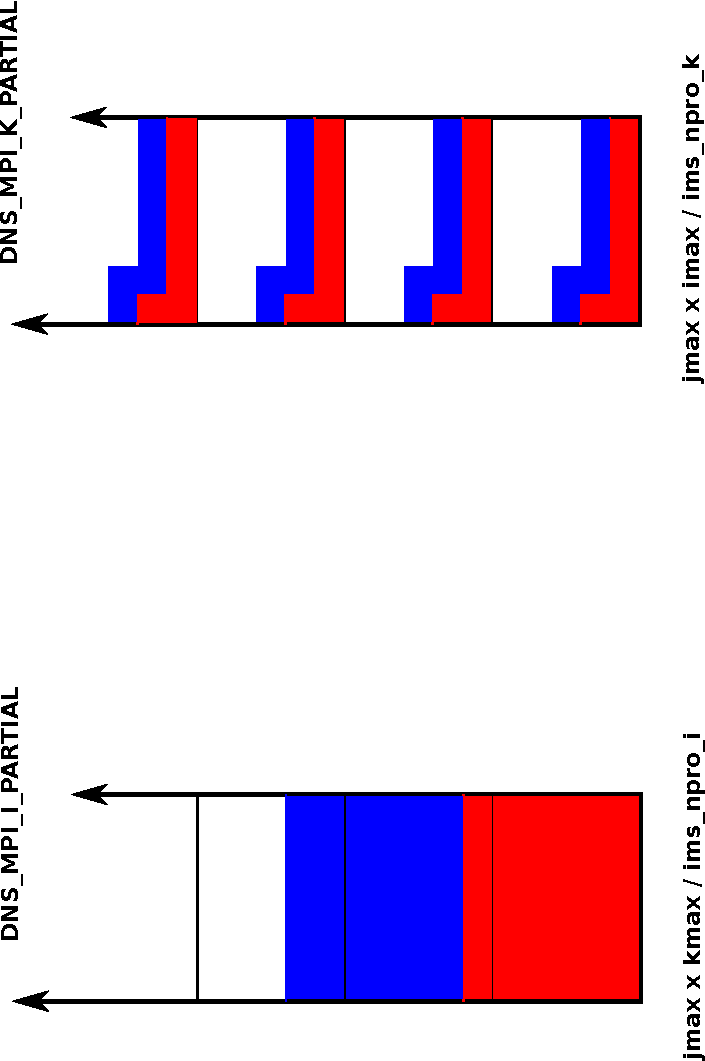
\includegraphics[height=0.8\textwidth,angle=270]{figs/parallel01b}
\caption{Memory management in transposition operations, from sketch in
  figure~\ref{fig:parallel01a}. Each color indicates the block of memory that
  goes into a common task. Based on these graphs, the offsets, strides and sizes
  in the MPI derived types are defined. The ratios at the bottom need to be an
  integer. You have as many colors as tasks involved in the corresponding
  transposition.}
\label{fig:parallel01b}
\end{centering}
\end{figure}

The I/O is done using MPI\_IO library. We read 
\begin{equation*}
{\tt ims\_npro}={\tt ims\_npro\_i} \times {\tt ims\_npro\_k} 
\end{equation*}
contiguous blocks of contiguous data, each block into one task. The
corresponding state is precisely equal to that obtained after the PARTIAL\_I
transposition, and so the only additional thing we need to do is an inverse
transposition of that type, and we already have the structure described in
figure~\ref{fig:parallel01a}. By this procedure we also defined the mapping,
which is sketched in figure~\ref{fig:parallel02}. From that mapping we see that
a task {\tt ims\_pro} contains the block given by
\begin{eqnarray*}
&{\tt ims\_pro\_i} = {\tt MOD(ims\_pro,ims\_npro\_i)}\\
&{\tt ims\_pro\_k} = {\tt INT(ims\_pro,ims\_npro\_i)}
\end{eqnarray*}

\begin{figure}[!ht]
\begin{centering}
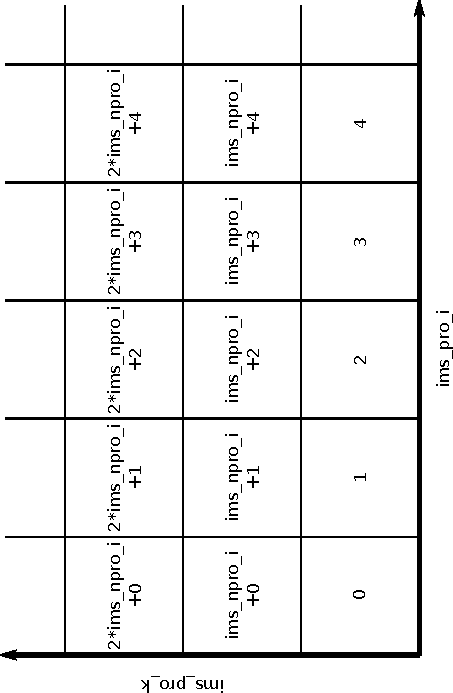
\includegraphics[height=0.6\textwidth,angle=270]{figs/parallel02}
\caption{Mapping.}
\label{fig:parallel02}
\end{centering}
\end{figure}

When needed, the information defining the boundary conditions is read from disk
using a similar procedure. we just need to define new MPI types for the
transposition along $Ox$ according to the specific size of the corresponding
arrays. This is done inside the I/O routines, as appropriate.

For the transpositions required in the Poisson equation, the procedure is
similar to the main algorithms defined above and shown in
figures~\ref{fig:parallel01a} and \ref{fig:parallel01b}, although two additional
planes in $Oy$ containing the boundary conditions, one at the bottom and one at
the top, and one in $Ox$ for the pseudo-Nyquist frequency are added (pseudo
meaning that only one should be added, but space is reserved in each processor
along that direction to keep the algorithm homogeneous; this could be
redefined). For these cases, padding is used inside each pages (defined above)
so that the only constraints in the grid are those imposed before in the two
major kinds of transposition. Hence, for a transposition along $Oz$, the same
structure as shown in figure~\ref{fig:parallel01b} is used but with a page of
size {\tt isize\_txc\_dimz} instead of {\tt imax}$\times${\tt jmax}, such that
{\tt isize\_txc\_dimz} is a multiple of 2$\times${\tt ims\_npro\_k}, (the factor
of 2 for real and imaginary parts of the same complex number to remain in the
same processor) and larger than ({\tt imax+2})$\times$({\tt jmax+2}). 

The same description applies to the transposition along $Ox$. The only
difference here is that a second type is added for the transformation without
the Nyquist frequency. This is used for instance for the first forward
transposition of data. {\em More here?}

\chapter{Scaling}\label{sec:scaling}

For spatial discretization implicit schemes are used. Hence, the calculation of
a derivative always involves communication amongst all processors in a line
along which a derivative is computed. From ad-hoc considerations it is not clear
which is the optimum two-dimensional domain-decomposition.  While for small
numbers of cores one would expect the network latency of an MPI call to
dominate, for larger numbers it is the number of processors involved in the call
that makes MPI calls expensive. Therefore, below a certain threshold, a 1D
decomposition is expected to be beneficial. Where this turnover takes place is
subject to many factors such as the CPU clock speed, network latency, MPI
implementation, number of grid points, etc.

We briefly introduce now definitions and notation used in the rest of this
section. We define $Q:=q_x\times q_y \times q_z$, the number of grid points, as
a measure of the size of the simulations and choose in the following to label
simulations by $Q$. To label the simulations, we use the common abbreviations
\begin{equation}
\kilo=2^{10};\qquad\mega=2^{20};\qquad\giga=2^{30}
\end{equation}
for readability. The memory necessary to save one 3D array in double precision
data format is $8\times Q~\mathrm{Byte}$.  The scaling of the code is discussed
in terms of speedup $S$ and efficiency $\eta$ defined as
\begin{equation}
 S:=\frac{T}{T_\mathrm{ref}}\qquad \eta = \frac{T}{NT_\mathrm{ref}} \times 100\%,
\end{equation}
where $T$ is the real time to run a particular case, $N$ the number of
processors and the subscript 'ref' indicates a reference value.

The code has been instrumented to measure the real time that is necessary to
perform one stage of the multi-stage Runge-Kutta time-stepping scheme.  This
corresponds essentially to the evaluation of the right-hand-side term of the
governing equations solved. The pre-processor flag \verb,-DUSE_PROFILE,
activates it and data is written into the log file \verb,dns.log,. The aim is to
remove the overhead time associated with I/O and initialization.

\section{Scaling on the cluster \texttt{jugene@fz-juelich.de}}

Performance of the DNS code has been measured for various geometries varying the
total number of grid points by two orders of magnitude. Many-core scaling
properties of the DNS code, version 5.6.6 on the
machine \texttt{jugene@fz-juelich.de} (site J{\"u}lich Supercomputing Center)
were investigated. All simulations have been run in SMP mode using 4 OpenMP
threads, reaching up to up to 8k MPI tasks distributed over 8k nodes (1 rack
contains 1k nodes), using 4 cores per node (i.e. 32k cores in total). Linear
scaling is observed for up to 4096 MPI tasks using about 6-8 \mega~grid points
per processor (domains of 24-32 \giga~grid points).  The maximum efficiency is
usually reached when simulations are carried out within one mid-plane. In this
case, a slightly super-linear scaling (with respect to the reference at 32
nodes) is observed for the standard domain sizes of up to 4 \giga~grid points.

\begin{table}[!ht]
\begin{centering}
\begin{tabular}{p{2cm} p{0.5cm} p{0.5cm} p{0.5cm} p{1.cm} }
\toprule
Name& $q_x$& $q_y$& $q_z$& $Q$\\
\midrule
\texttt{1024x0384}& 1024& 1024&  384& 384 \mega\\
\texttt{2048x0192}& 2048& 2048&  192& 768 \mega\\
\texttt{2048x1024}& 2048& 2048& 1024&   4 \giga\\
\texttt{3072x1536}& 3072& 3072& 1536&  12 \giga\\
\texttt{4096x1536}& 4096& 4096& 1536&  24 \giga\\
\texttt{4096x2048}& 4096& 4096& 2048&  32 \giga\\
\bottomrule \\
\end{tabular}\\
\caption{Geometry and labels of the 3D cases.}
\label{tab:sim_table}
\end{centering}
\end{table}

The code has been run for 2 iterations, i.e. 10 Runge-Kutta stages using the
fourth-order, five-stages algorithm, and the variance of measured times was
found to be of the order of 1\%.  The cases considered here are listed in
Table \ref{tab:sim_table}.

\subsection{Strong Scaling}\label{sec:domain_decomposition}

The total number of MPI tasks (nodes) available to a simulation are distributed
as $N = $\texttt{ims\_npro} = \texttt{ims\_npro\_k}
$\times$ \texttt{ims\_npro\_i} in the directions of $k$ ($z$) and $i$ ($x$). A
series of measurements has been carried out to determine the optimum
configuration for the six cases listed in table
\ref{tab:sim_table}. Scaling matrices are shown in Figures \ref{fig:matrices1}
and \ref{fig:matrices2} for the different cases.  In these matrices the number
of processors is constant along diagonals from the lower left to the upper
right. In every matrix, the diagonal for $N=1k$ MPI tasks is outlined by solid
borders. In each of these diagonals, the best and worst configurations are
marked by green, respectively red, color. In these matrices, the speed-up and
efficiency is for strong scaling, and always calculated with respect to the time
$T_\text{ref}$ for the lowest number of cores with the
lowest \texttt{ims\_npro\_i}. Efficiency $\eta$ and speed-up $S$ are calculated
as above. The shapes used in the simulations, that is, the relative connection
among mid-planes, is $1\times 1\times 1$, $2\times 1\times 1$, $2\times 2\times
1$, $2\times 2\times 2$, $4\times 2\times 2$, ordered from 1 mid-plane (512
nodes) to 16 mid-planes (8192 nodes).

\begin{figure}
\begin{centering}
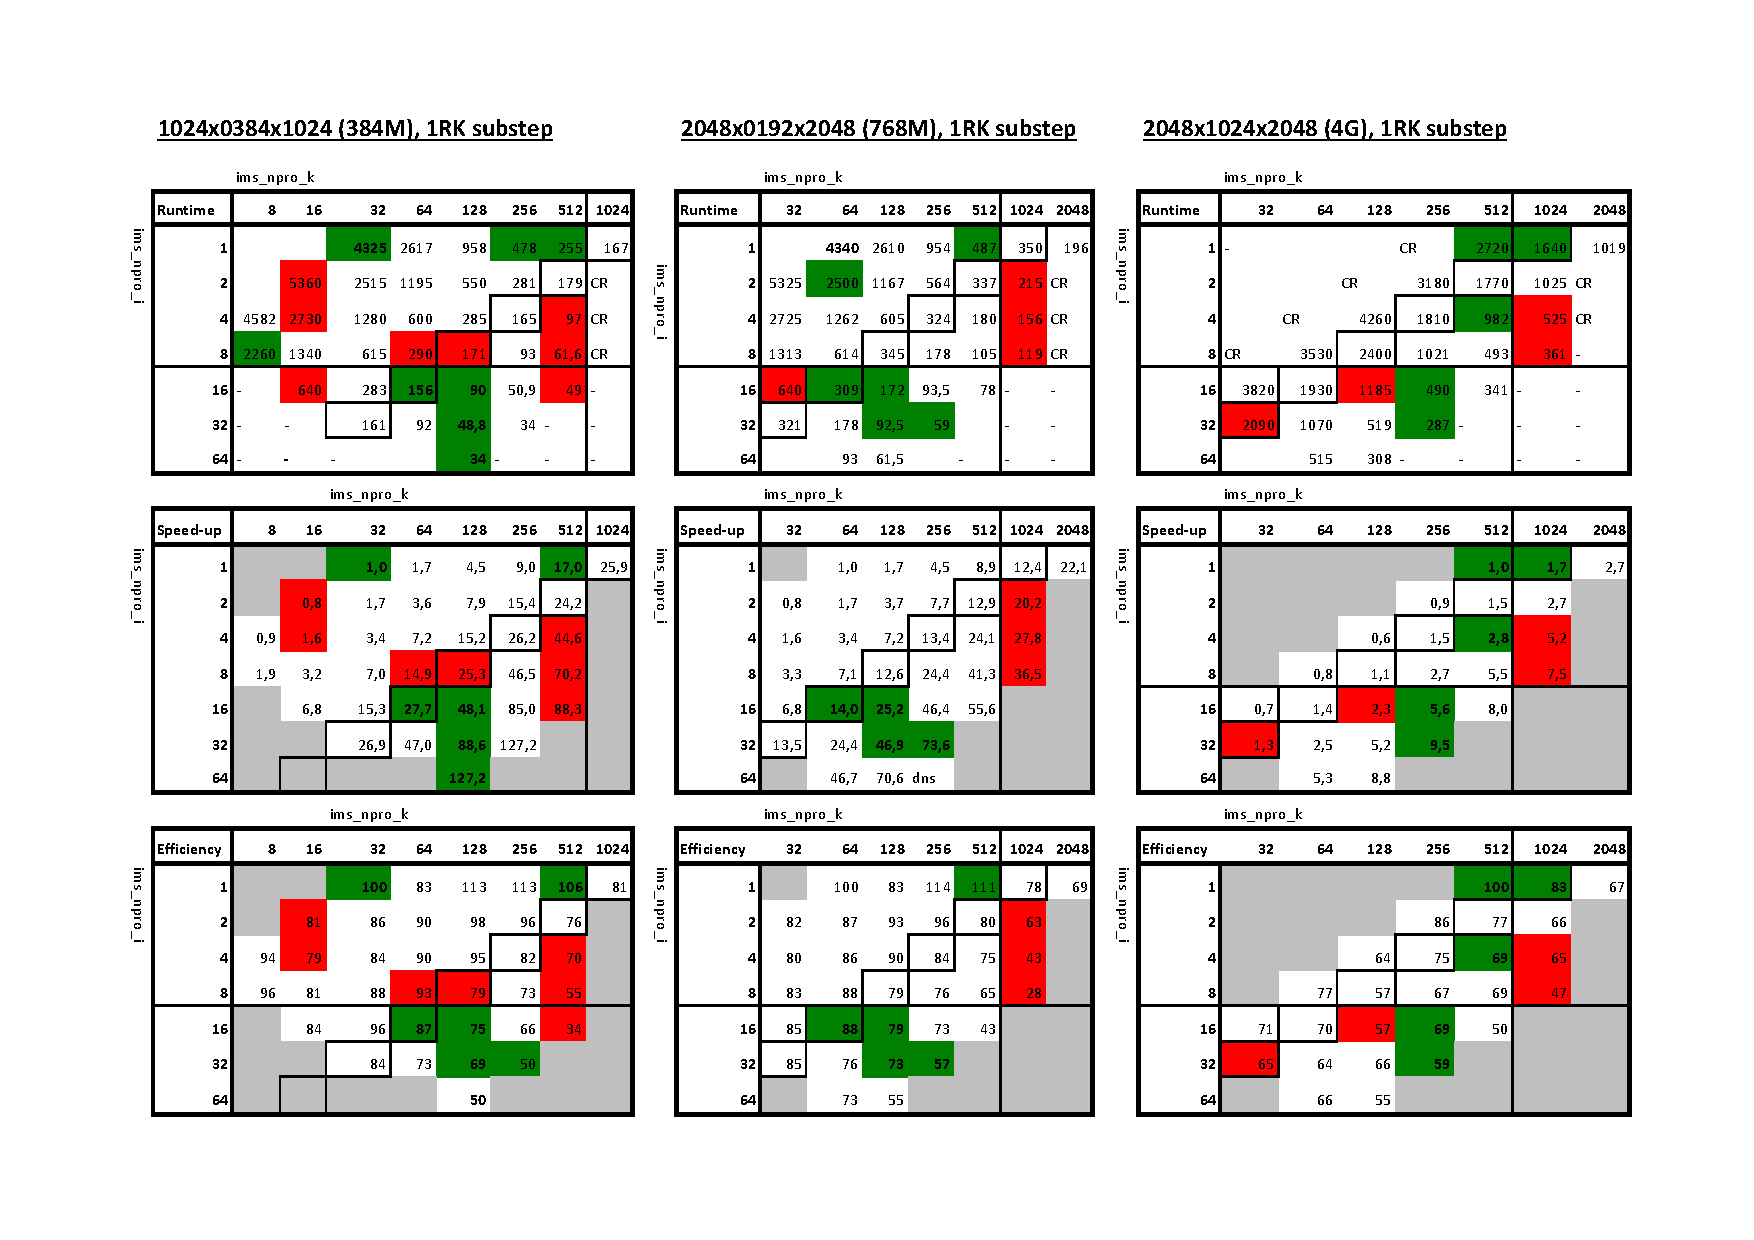
\includegraphics[height=0.9\textwidth,angle=90]{figs/matrices_1.pdf}
\caption{Matrices for scaling and 2D domain decomposition. Time is in hundredth
  of a second per single Runge-Kutta stage. In the time-matrices, simulations
  that crashed because of too little memory (above diagonals) and page problems
  (below diagonals) are marked by \texttt{CR}. If no measurement for a certain
  configuration was attempted, the cell is left empty. For speed-up and
  efficiency all configurations not available are marked gray.}
\label{fig:matrices1}
\end{centering}
\end{figure}

\begin{figure}
\begin{centering}
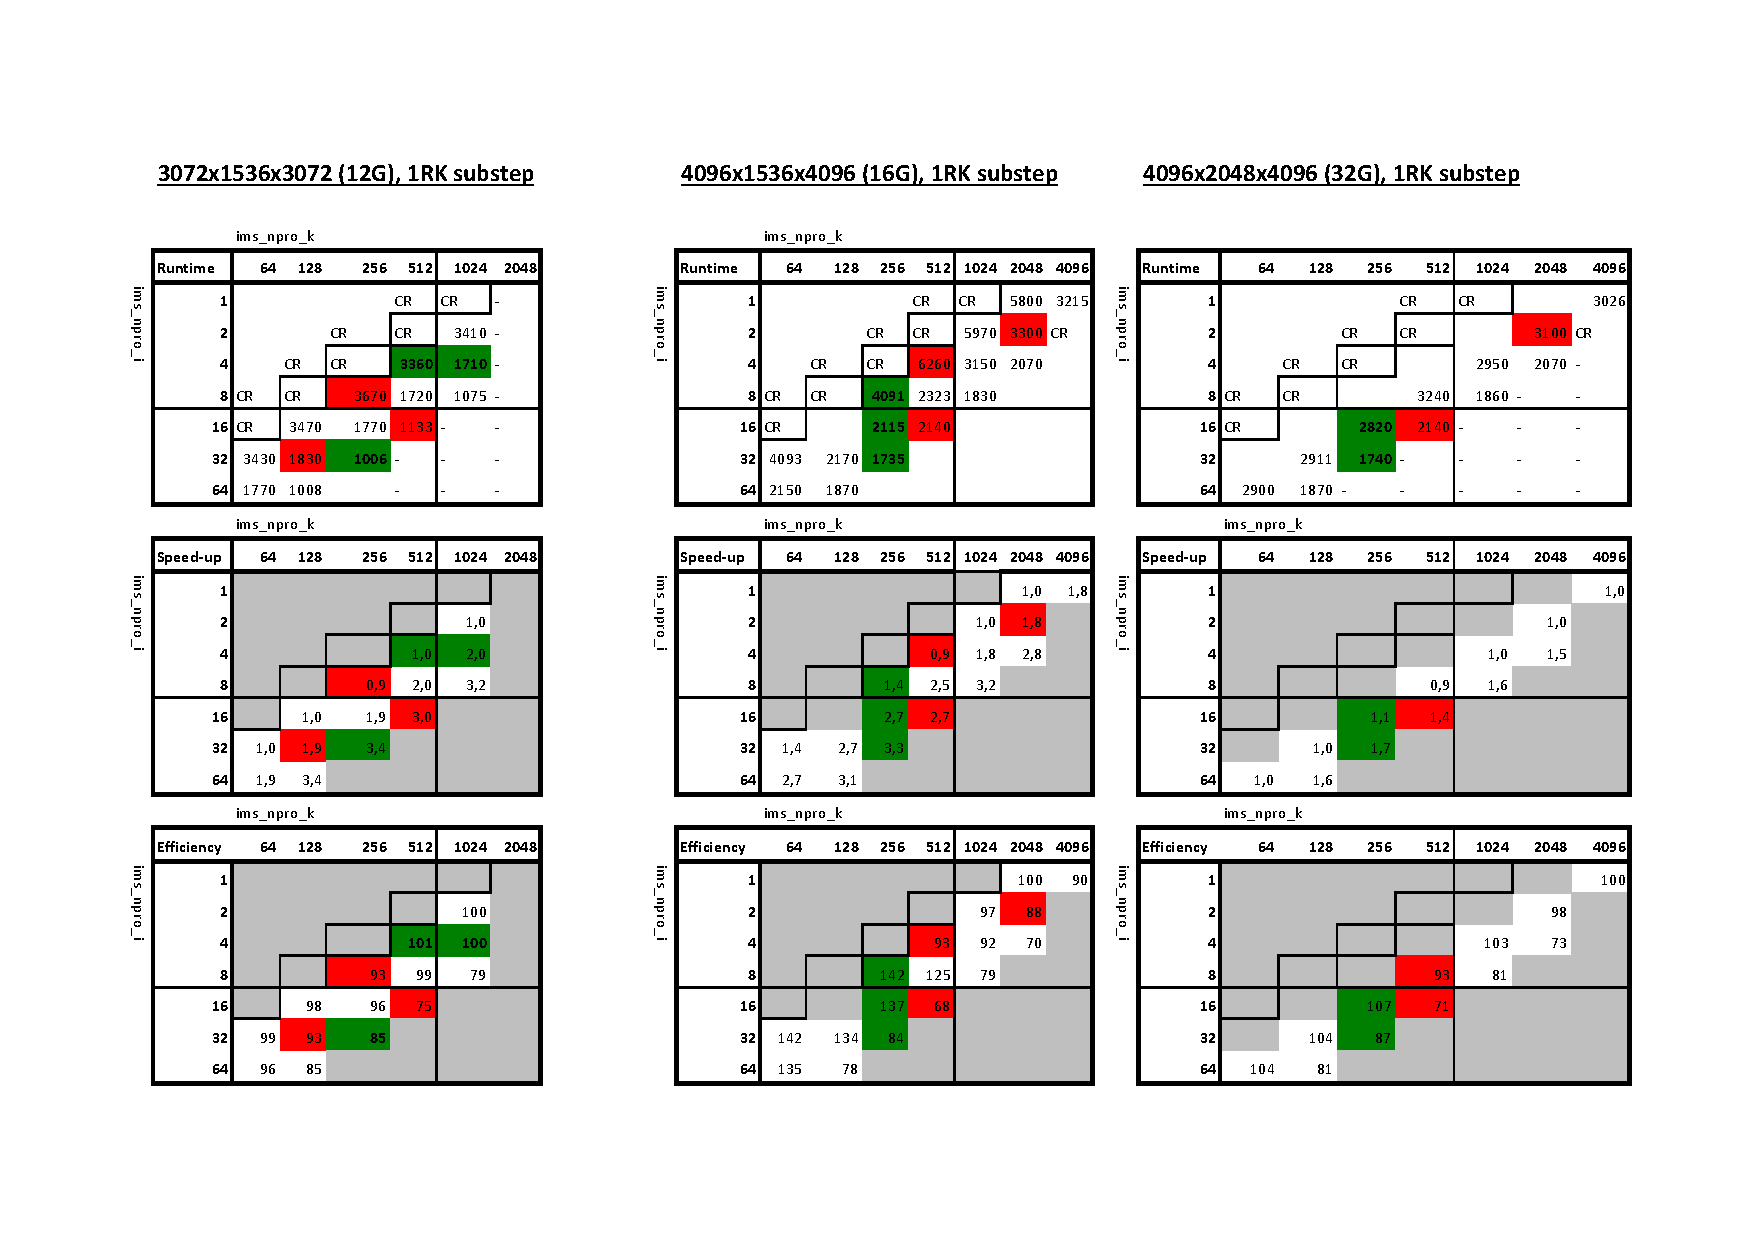
\includegraphics[height=0.9\textwidth,angle=90]{figs/matrices_2.pdf}
\caption{More cases. Same legend as in Figure~\ref{fig:matrices1}.}
\label{fig:matrices2}
\end{centering}
\end{figure}

\subsection{Scaling from 32 to 8192 nodes}

A strong scaling analysis over the entire range of nodes from 32 to 8192 is not
possible. Hence, we restrict ourselves to a scaling analysis where we consider
the number of grid points that is handled per processor and time unit. A
straightforward definition for a metric of performance $P$ is
\begin{equation}
  P:=\frac{Q}{N T} \;,
\end{equation}
the number of grid points processed per node and per time. $T$ is the time
needed by each of the cases to advance exactly the same amount of instructions
in the main algorithm, e.g. one stage of the Runge-Kutta scheme. $P$ is a metric
that makes performance comparable over \textit{almost} arbitrary problem sizes
and numbers of cores.

Note, that the caveat here is the operation count for the Fourier transforms
which goes as $q_i \log q_i$ and $q_i \approx Q^{1/3}$ if domains are expanded
by the same factor in each direction. Hence, for the overall operation count of
the Fourier transforms $\Sigma_\mathrm{FFT}$ we get
\begin{equation}
\frac{\Sigma_{\mathrm{FFT}}}{q_{i}^{2}}\propto 3 q_i \log q_i = Q^{1/3} \log
Q\Rightarrow \Sigma_\mathrm{FFT}\propto Q\log Q.
\end{equation}
For the range of $Q$ considered here, this effect is, however, small since the
super-linear contribution of $\Sigma_\mathrm{FFT}$ is only $\frac{\log 32\giga
}{\log 384\mega} \approx 1.2$ and the FFT accounts for a negligible part of the
computational time ($1\%-5$\% of the computational part, which is
$0.5$\%-$2.5$\% of the overall time).  The operation count of the rest of the
algorithms is linear.

Given $P$, one can compute a virtual efficiency and speed-up $\eta_v$ and $S_v$ as
\begin{equation}
\eta_v:=\frac{P}{P_\mathrm{ref}}; \qquad S_v:=\frac{N}{N_\mathrm{ref}}\frac{P}{P_\mathrm{ref}}
\end{equation}
with respect to a reference. Here, we use the same reference for all simulations
and cases, namely, the \texttt{32 x 1} decomposition of the case with
$Q=384$ \mega. For larger numbers of cores $N$ and simulation sizes $Q$ we
always choose the optimum configuration which is marked by green color in
Figures \ref{fig:matrices1} and \ref{fig:matrices2}.

\begin{figure}
\begin{centering}
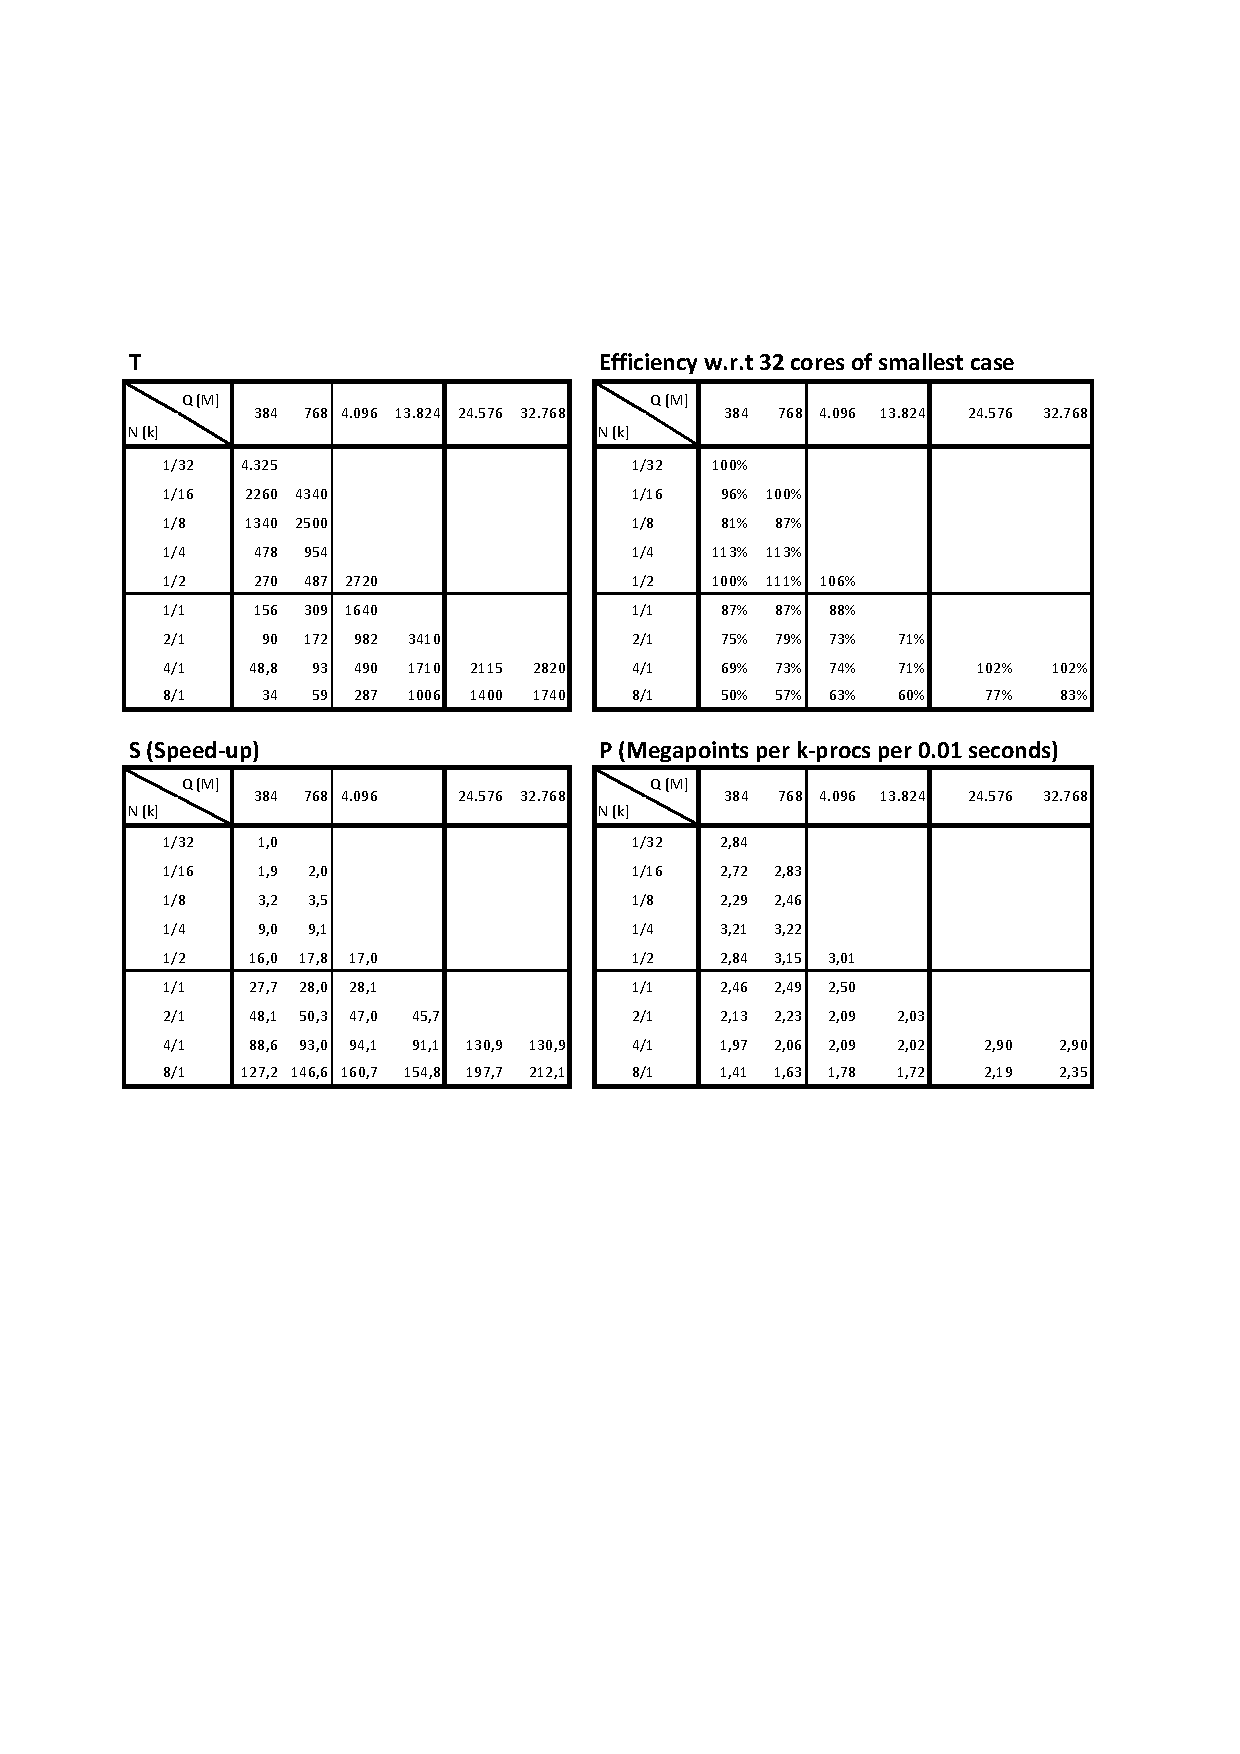
\includegraphics[width=1.0\textwidth]{figs/scaling_overview.pdf}
\end{centering}
\caption{Scaling results in term of Speed-Up $S_W$, Efficiency $E_W$ and
Performance $P$ as defined above.}
\label{fig:v_scaling1}
\end{figure}

The scaling as described in the above paragraph is summarized in the tables
shown in Figure \ref{fig:v_scaling1}. The first table contains the real time
needed for one Runge-Kutta stage, measure in hundredths of a second. As already
said before, these data is simply collected from the matrices on
Figures \ref{fig:matrices1} and \ref{fig:matrices2}. The other 3 tables in
Figure \ref{fig:v_scaling1} contain the corresponding values of $P$, $\eta_v$
and $S_v$.  Figure \ref{fig:v_scaling2} shows the speed-up $S_v$. In the upper
panel there is one line for each cases.  Note, that the definition of $S_v$
does \textbf{not imply that cases start on the linear scaling line}. In this
case, it is part of the measurements and simply means that $\eta_v\approx 100\%$
or $P\approx P_\mathrm{ref}$.

\begin{figure}
  \begin{centering}
  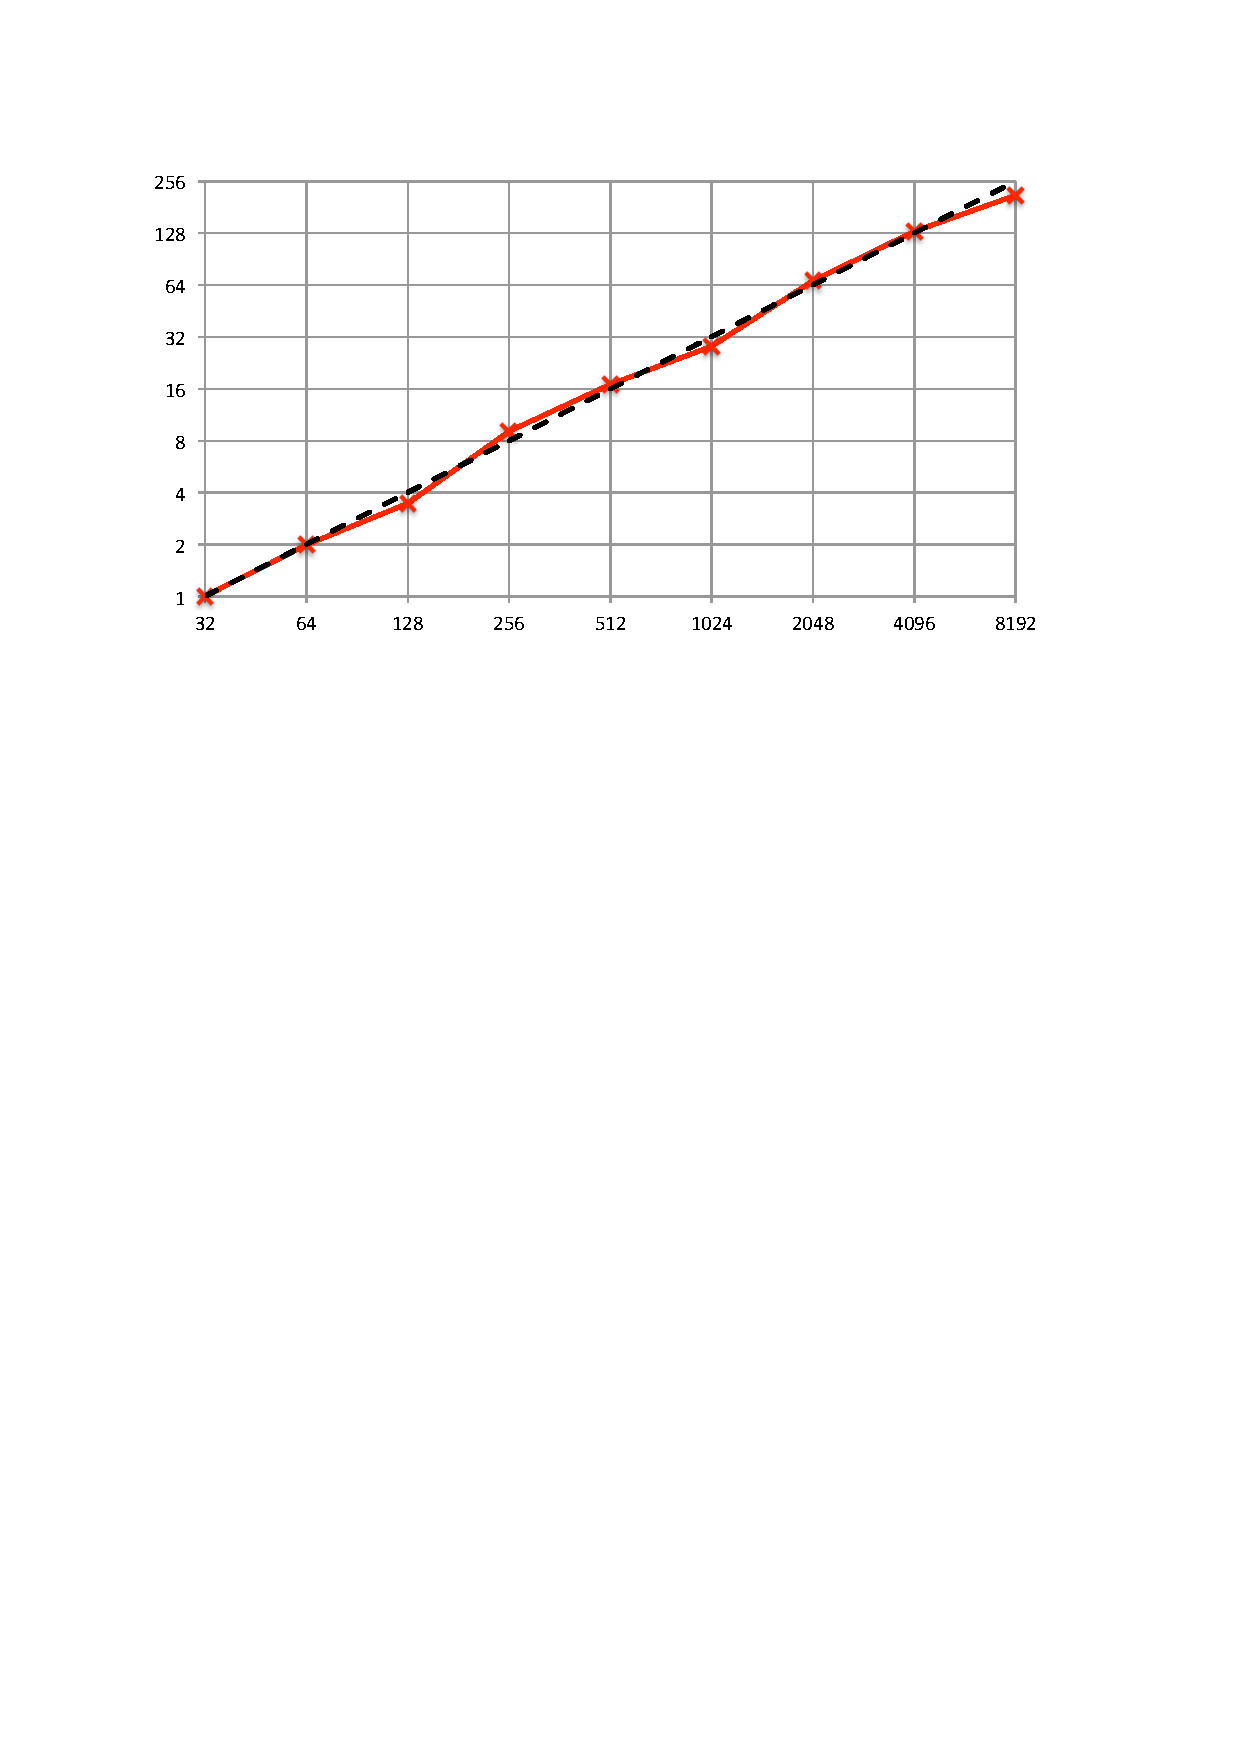
\includegraphics[width=0.5\textwidth]{figs/weak_scaling1.pdf}%
  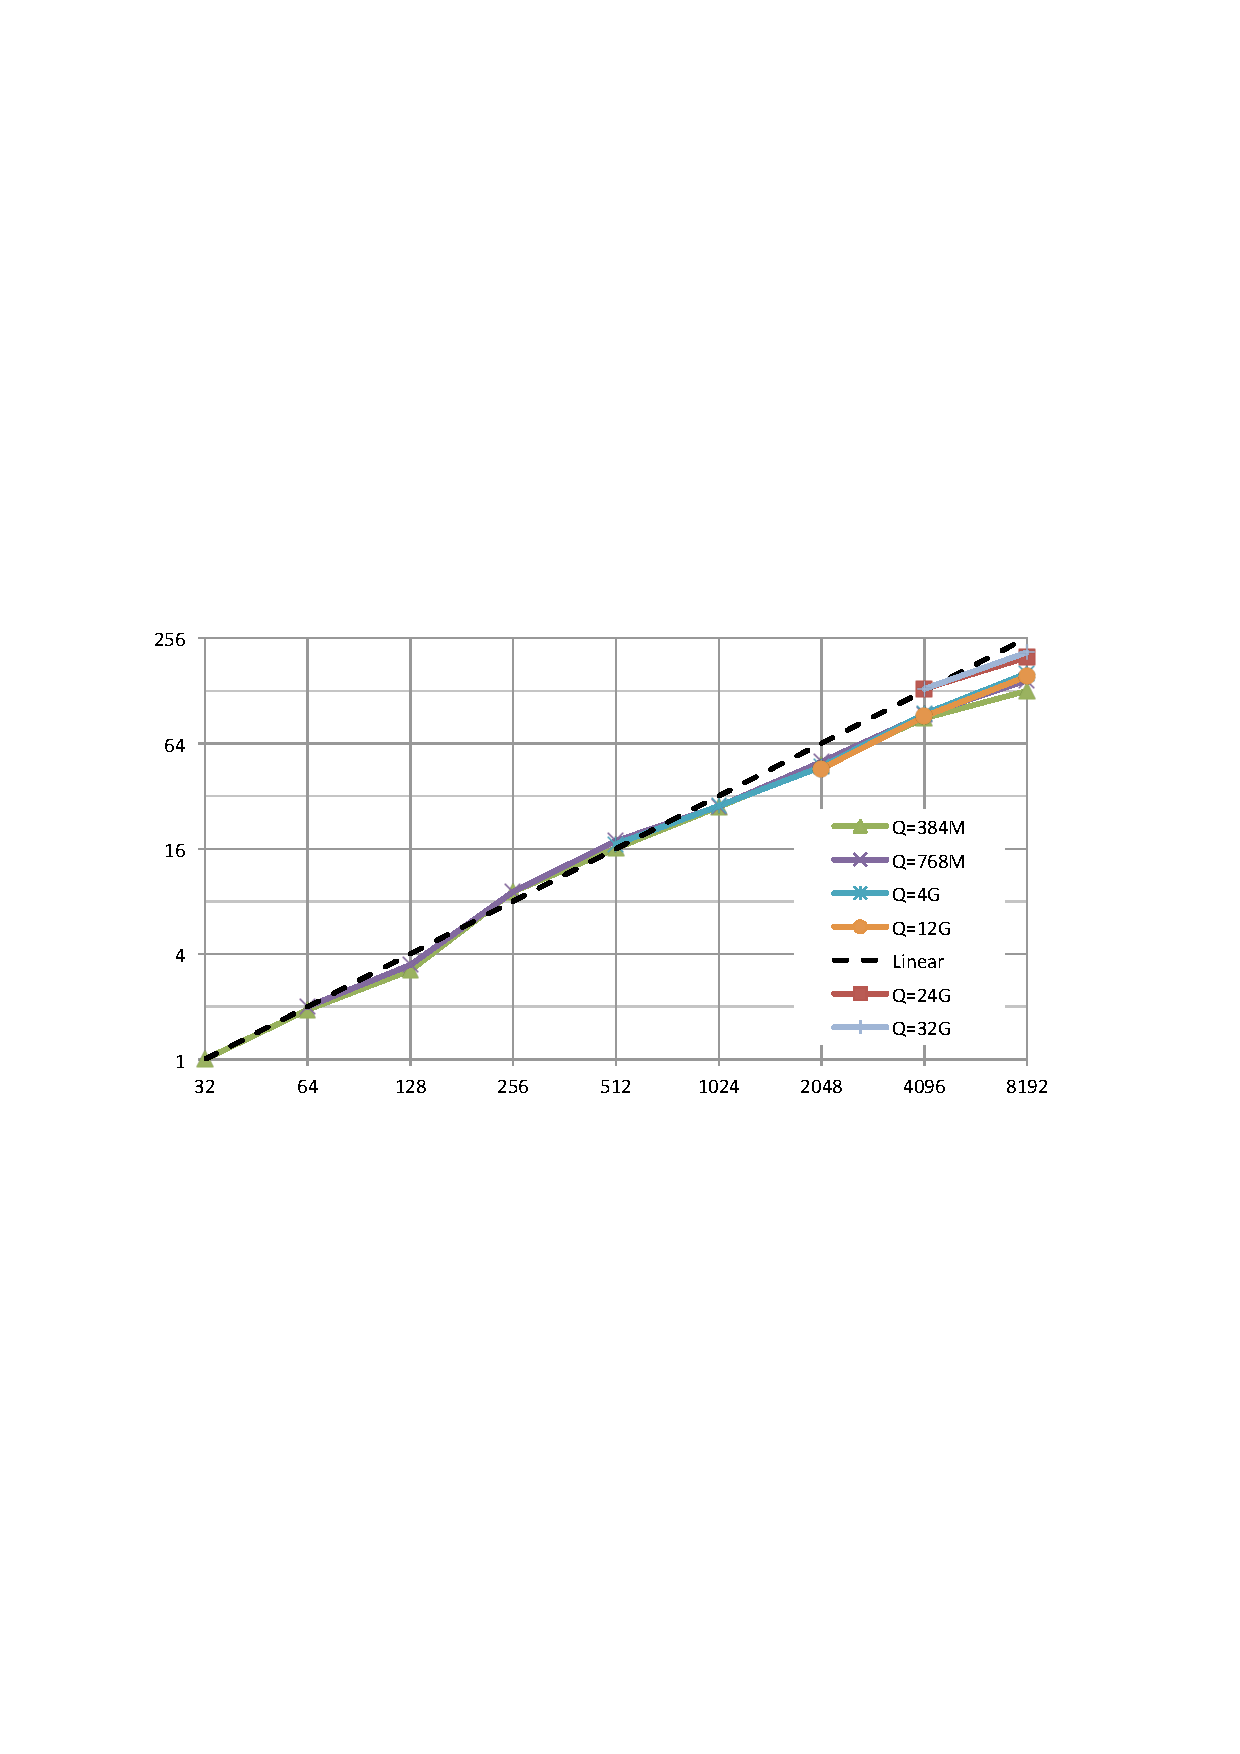
\includegraphics[width=0.5\textwidth]{figs/weak_scaling2.pdf}\\
  \end{centering}
  \caption{Upper panel: $S_W$ versus number of nodes for all geometries. Lower
    panel: maximum speedup for a given number of processors $\max(S_W)|_N$; axes
    as in upper panel.  }
  \label{fig:v_scaling2}
\end{figure}


\section{Scaling on the cluster \texttt{juwels@fz-juelich.de}}

With two sockets each holding 24 CPU cores, juwels features 48 physical cores per node and thus
introduces a single prime factor three to the number CPUs available. To optimally utilize this,
domain sizes should also contain a prime factor three.

The cluster is heterogeneous and features
\begin{itemize}
  \item[(1)] a partition \texttt{batch} with 2271 standard-memory nodes (2x24 cores, 96 GB )
  \item[(2)] a partition \texttt{mem192} with 240 enhanced-memory nodes (2x24 cores, 192 GB )
  \item[(3)] a booster module with 56 GPU-accelerated nodes ( 2x20 cores + 4 GPUs, 192 GB; to be extended in 2020).
\end{itemize}

Scaling was tested using up to 512 nodes on the \texttt{batch} partition (Tab.~\ref{tab:scaling_juwels} and Fig.~\ref{fig:scaling_juwels}
and up to 64 nodes of the \texttt{mem192} partition (Tab.~\ref{tab:memory_juwels}).
There appears to be a significnat memory-overhead of the underlying MPI
which sometimes enables to run particular cases in much less than half the number of large-memory nodes as compared
to running the same configuration in the \texttt{batch partition}.

In comparison with juwels, the normaliezd performance (CPU-h per $1024^3$ points per iteration) is better by up to a factor of $3$, but only for relatively small cases that can be run within a few (up to 4) nodes. For operational cases (using 32 to 128 nodes), the performance boost is around $2$. For even larger cases utilizing 256 or more nodes, performance boost in comparison with juwels is smaller than 2, and it approaches one from above for jobs using 10000 or more MPI tasks.
%
\begin{table}
  \caption{Scaling of two cubed cases in the batch partition of \texttt{juwels@fz-juelich.de}; only computation no initialization, no I/O}
  {\footnotesize\begin{tabular}{r | r r r | r r r | rrr}
    \toprule
    Case   & \multicolumn{3}{c|}{$1536^3$} & \multicolumn{3}{c}{$3072^3$}\\
    \midrule
    \#nodes&        time/it $[s]$ & Speed-up & Eff. & Time/it $[s]$ & Speed-up & Eff.\\
    \midrule
                        8 &      113.5&   1.0&  1.00 \\
    \rowcolor{gray!20} 16&        57.5&   2.0&  0.99\\
                       32&        36.3&   3.1&  0.78\\
    \rowcolor{gray!20} 64&        21.2&   5.4&  0.67& 163.0& 1.0& 1.00\\
                       96&        15.1&   7.5&  0.63&  98.4& 1.7& 1.10\\
    \rowcolor{gray!20}128&        11.5&   9.9&  0.62&  92.8& 1.8& 0.88\\
                      192&         9.1&  12.5&  0.52&  65.1& 2.5& 0.83\\
    \rowcolor{gray!20}256&         6.7&  16.9&  0.53&  51.4& 3.2& 0.79\\
                      384&                        &&&  38.1& 4.3& 0.71\\
    \rowcolor{gray!20}512&                        &&&  29.3& 5.6& 0.70\\
    \bottomrule
  \end{tabular}}
  \label{tab:scaling_juwels}
\end{table}

\begin{table}
  \caption{Average timing for total production jobs in the large-memory partition as compared to the batch partition.
  The batch case using 128 nodes is the smallest configuration for which the case runs in the batch queue. }
  \begin{centering}{\footnotesize\begin{tabular}{rrr|r|rrr}
    \toprule
    Partition               && \multicolumn{4}{c}{mem192}&batch\\
    \#nodes                 &[1]&    20  &  24  &  32 &  64 & 128\\
    \midrule
    \rowcolor{gray!20}\#tasks per node        &[1]&    16  &  48  &  48 &  48 &  48\\
    Wall-clock time/it &[s]      &    422 &  286 & 230 & 115 & 76 \\
    \rowcolor{gray!20} Memory used / node& [GB] &    187 &  160 & 124 &  81 & 52 \\
    total memory & [TB]       &    3.65&  3.75& 3.88& 5.06& 6.5\\
    \rowcolor{gray!20}node-h / it & [h]             &    2.34& 1.91 & 2.04& 2.05& 2.70\\
    \midrule
    Speed-up w.r.t. batch & $[$\%$]$  &    11& \cellcolor{green!62}{\textbf{31}}&22&22&  -\\
    \midrule\bottomrule

  \end{tabular}}\\\end{centering}
  \label{tab:memory_juwels}
\end{table}


\begin{figure}
  % \centering\includegraphics[width=0.66\textwidth]{figs/strong_scaling_juwels.pdf}
  MISSING FIGURE
  \caption{Strong scaling on juwels (solid lines); dashed lines indicated weak scaling.}
  \label{fig:scaling_juwels}
\end{figure}

\section{Scaling on the cluster \texttt{blizzard@dkrz.de}}

To be done.

\chapter{Profiling}\label{sec:profiling}

We include here results from profiling to identify where to put the effort to further optimize the code. The diagrams shown below have been constructed with {\tt gprof2dot.py}\footnote{\url{https://github.com/jrfonseca/gprof2dot}}.

\begin{figure}[H]
  \centering
  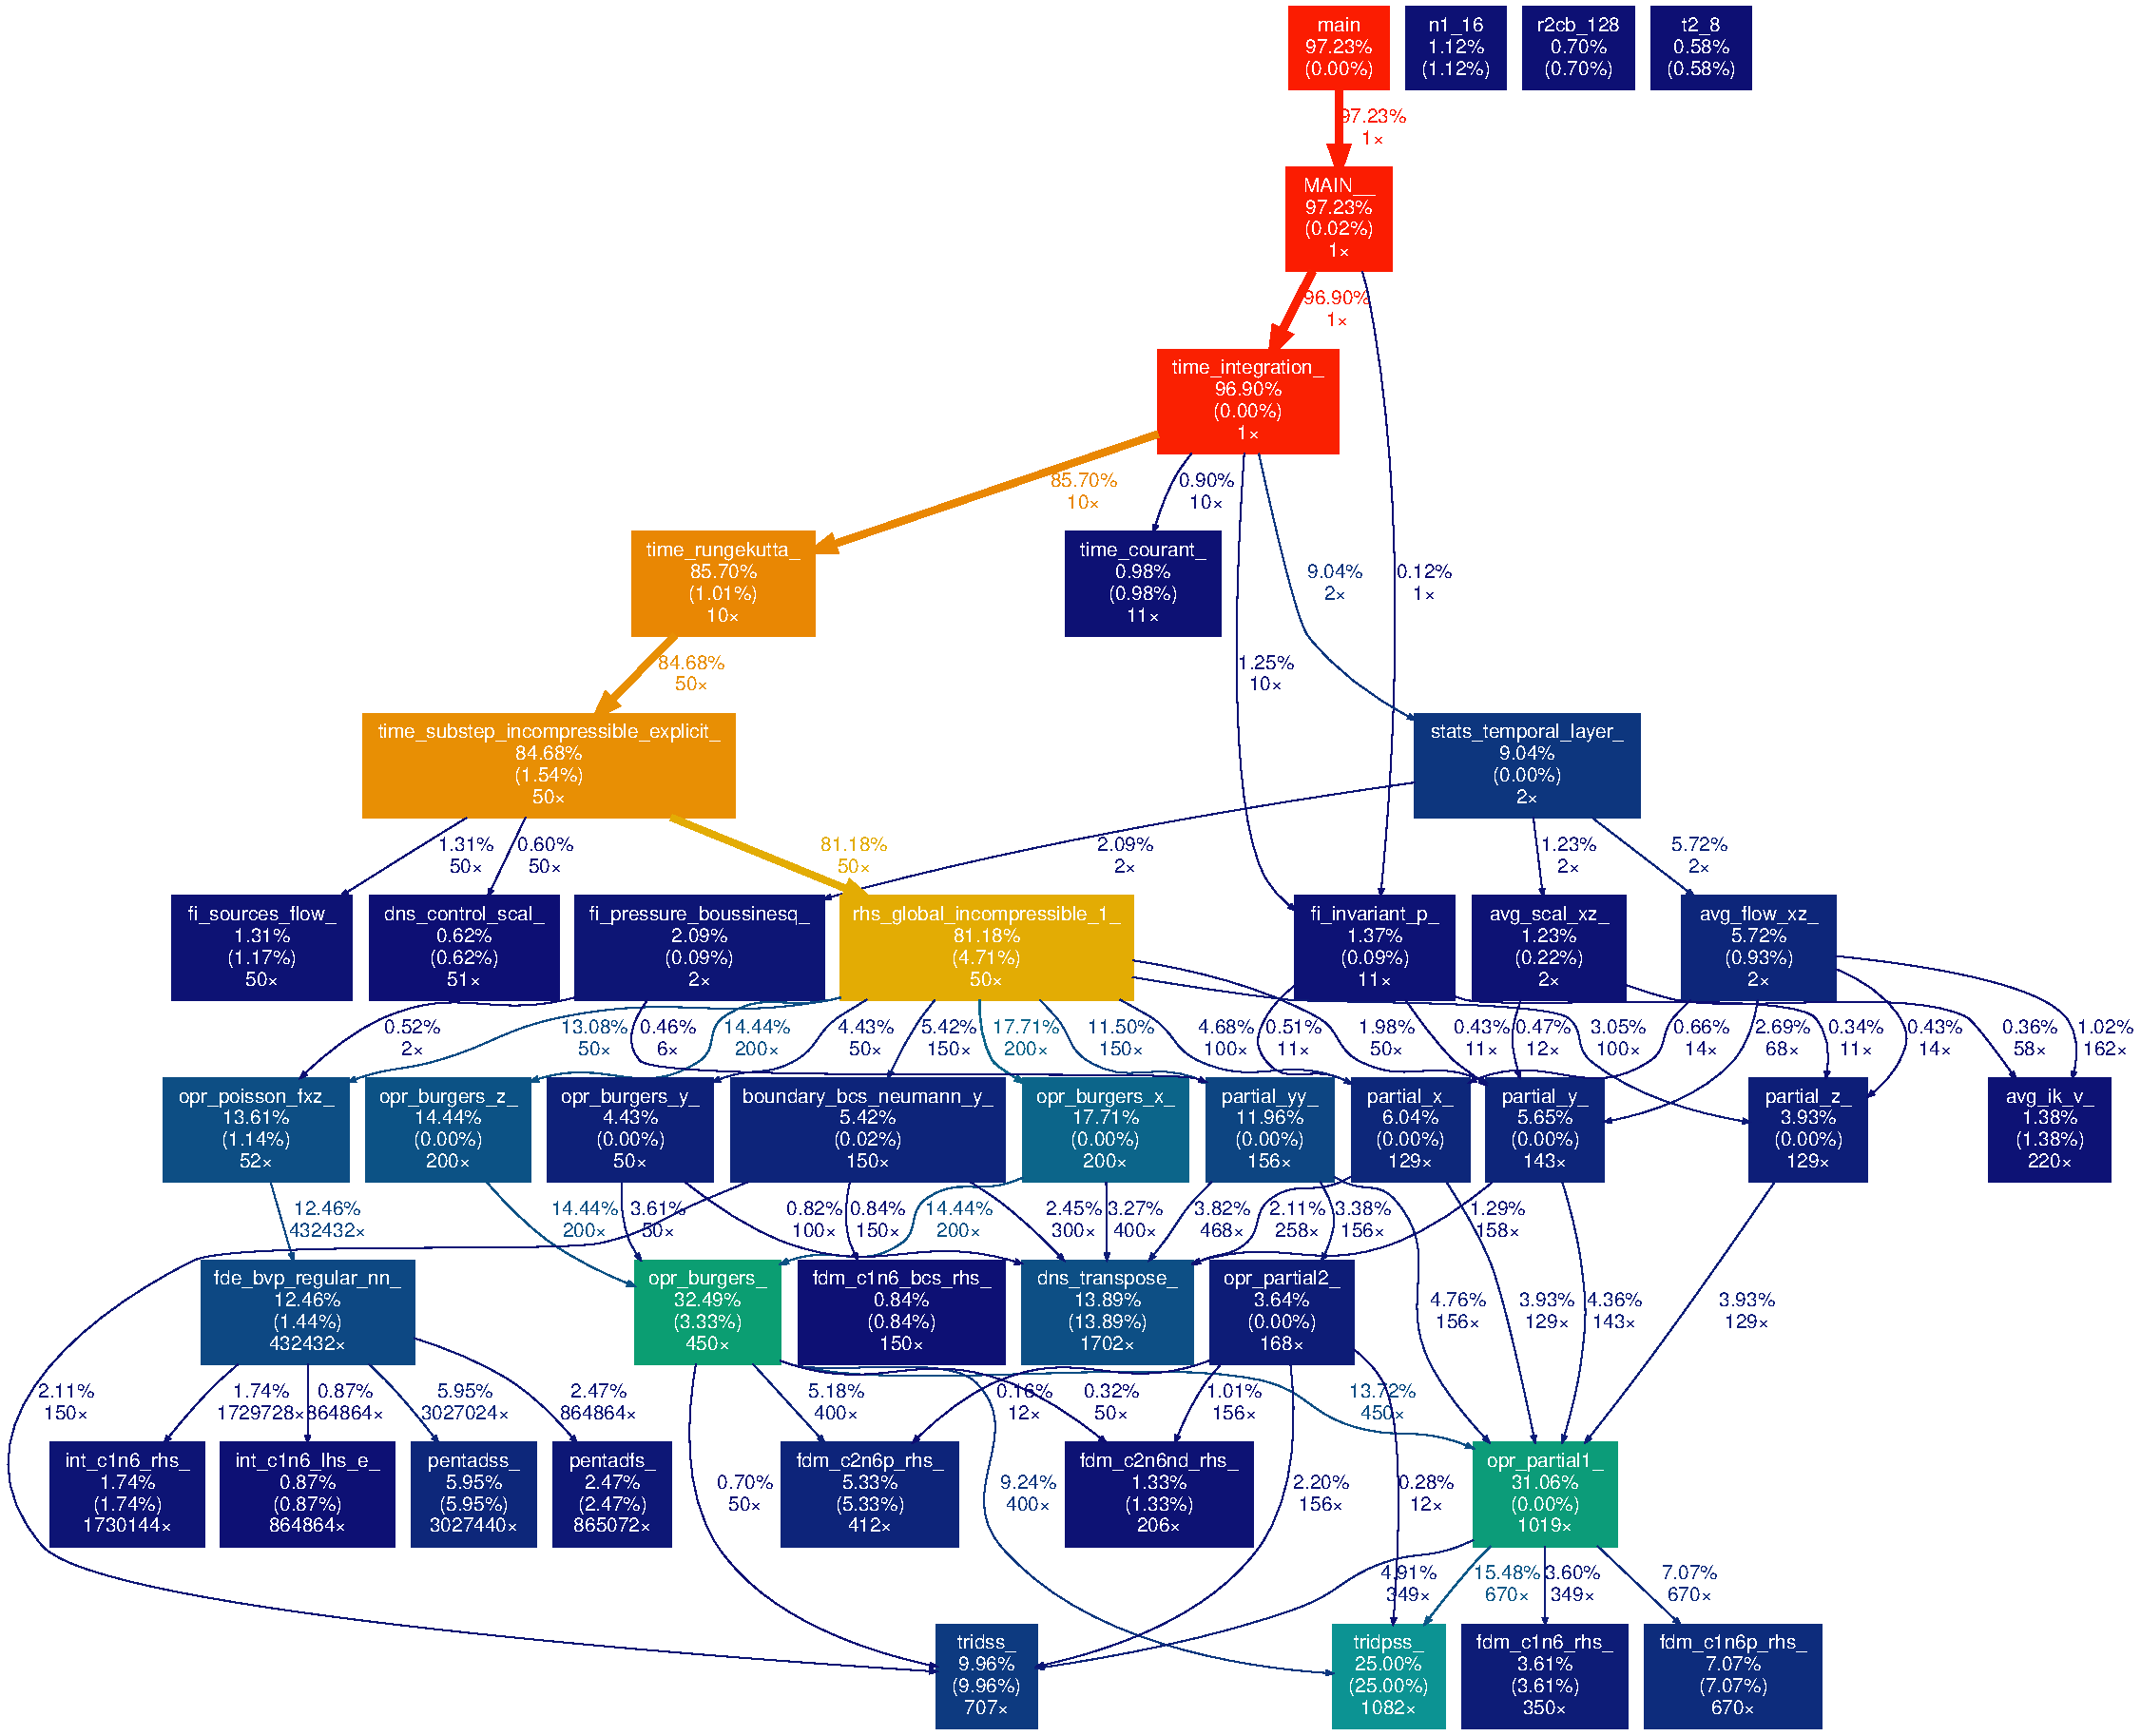
\includegraphics[clip,width=\textwidth]{figs/profiling.pdf}
  \caption{From {\tt example/Case33} running 10 iterations. Profiling data obtained from {\tt gfortran -pg} and processed with {\tt gprof}, running the command {\tt gprof path/to/your/executable | gprof2dot.py | dot -Tpdf -o output.pdf}.}
\end{figure}



\backmatter
\bibliographystyle{plainnat}
\bibliography{biblio.bib}

\end{document}
